%!TEX root = ../Pflichtenheft.tex

\chapter{Graphical User Interface}\label{ch:ui}
This chapter provides an overview of the \textit{\hyperref[abr:GUI]{GUI}} that is provided by the the system. \newline
While the designed interface is detailed and has been created implementation-near, it is not indented to be a pixel-perfect replica of the interface, but rather an example of how the interface may look like.
Aspects like spacing, texts, colors or layout choices are subject to change. \newline
Sections \ref{sec:navigation}, \ref{sec:screens} and \ref{sec:modals} present screens and modals for the web-interface, while section \ref{sec:email} presents the design of the emails sent to the user.

\section{Navigation}\label{sec:navigation}
The user will be able to navigate around the app using a so-called \textit{Navigation Drawer} \footnote{https://m3.material.io/components/navigation-drawer/overview}. \newline
A navigation drawer is a section of a web-app that is usually aligned on the start of the main layout (horizontally) and gives a user a list of navigation destinations to jump to. \newline
In a scenario of a wide viewport, like a \textit{Desktop} or \textit{Tablet} device, this navigation rail will always be visible to the user. \newline
In the scenario of a narrow viewport, like a \textit{Mobile}, this navigation rail will be only visible after being toggled by the user, using a toggle-button at the top of the screen.
Due to this, the navigation rail won't be visible on the UI-drafts for mobile screens.
Figure~\ref{fig:ui_d_mobile_navigation_drawer_overlay} shows this overlay of the navigation drawer on mobile devices.

\begin{figure}
    \centering
    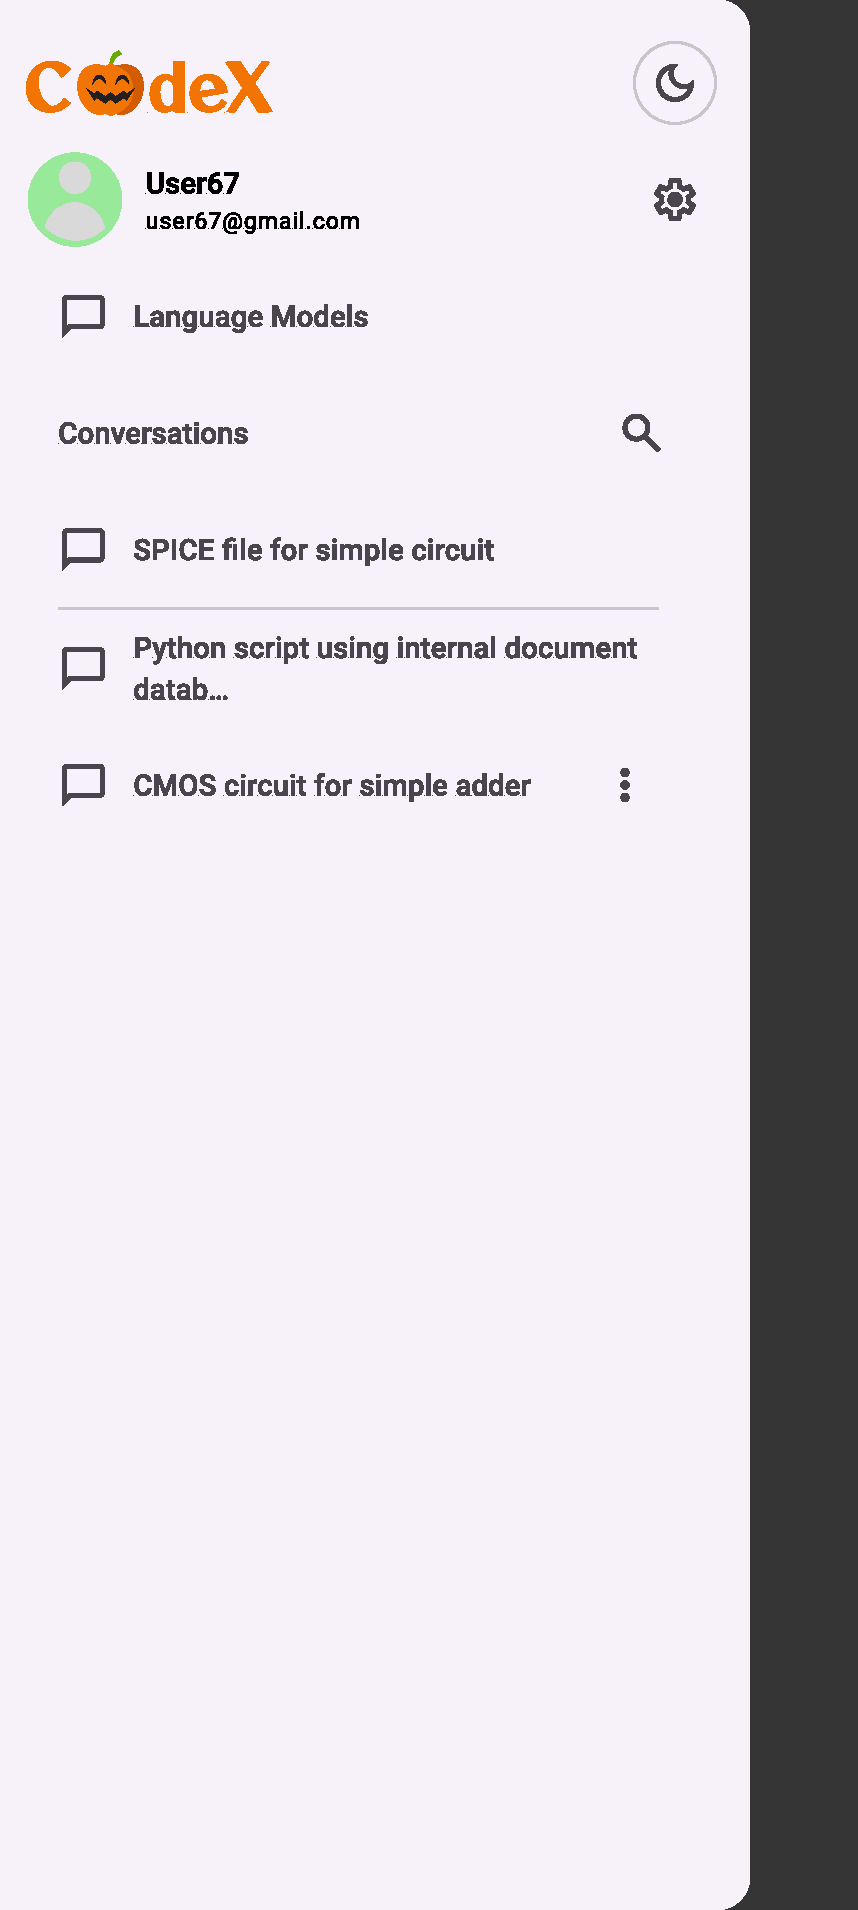
\includegraphics[width=5cm]{figures/ui/mobile/Navbar_Preview}
    \caption{\hyperref[abr:GUI]{GUI}: Navigation drawer overlay on mobile devices}
    \label{fig:ui_d_mobile_navigation_drawer_overlay}
\end{figure}

\section{Screens}\label{sec:screens}
Due to the different proportions of the possible screen sizes, each screen is presented as a \textit{Desktop} and \textit{Mobile} variant.
Whenever there is a link to a specific screen, the two variants are specified like the following: \texttt{<desktop\_variant>/<mobile\_variant>}.

\subsection{Conversation screen}
The conversation screen is the main screen of the app.
Here, the user has access to a sidebar that contains the previous conversations, as well as options to visit the account settings and toggle the theme of the app. \newline
The main content is the interface to create requests.
Before sending a request (\ref{fig:ui_d_conversation_screen_initial}/\ref{fig:ui_m_conversation_screen_initial}), the user can select the target language and \textit{\hyperref[abr:LLM]{LLM}}.
While the request is processing (\ref{fig:ui_d_conversation_screen_loading}/\ref{fig:ui_m_conversation_screen_loading}), a progress bar is shown.
When the request is finished, the user can either see the raw code (\ref{fig:ui_d_conversation_screen_not_visualized}/\ref{fig:ui_m_conversation_screen_not_visualized}) or visualize the code (\ref{fig:ui_d_conversation_screen_visualized}/\ref{fig:ui_m_conversation_screen_visualized}) if available for the specific language.

\begin{figure}
    \centering
    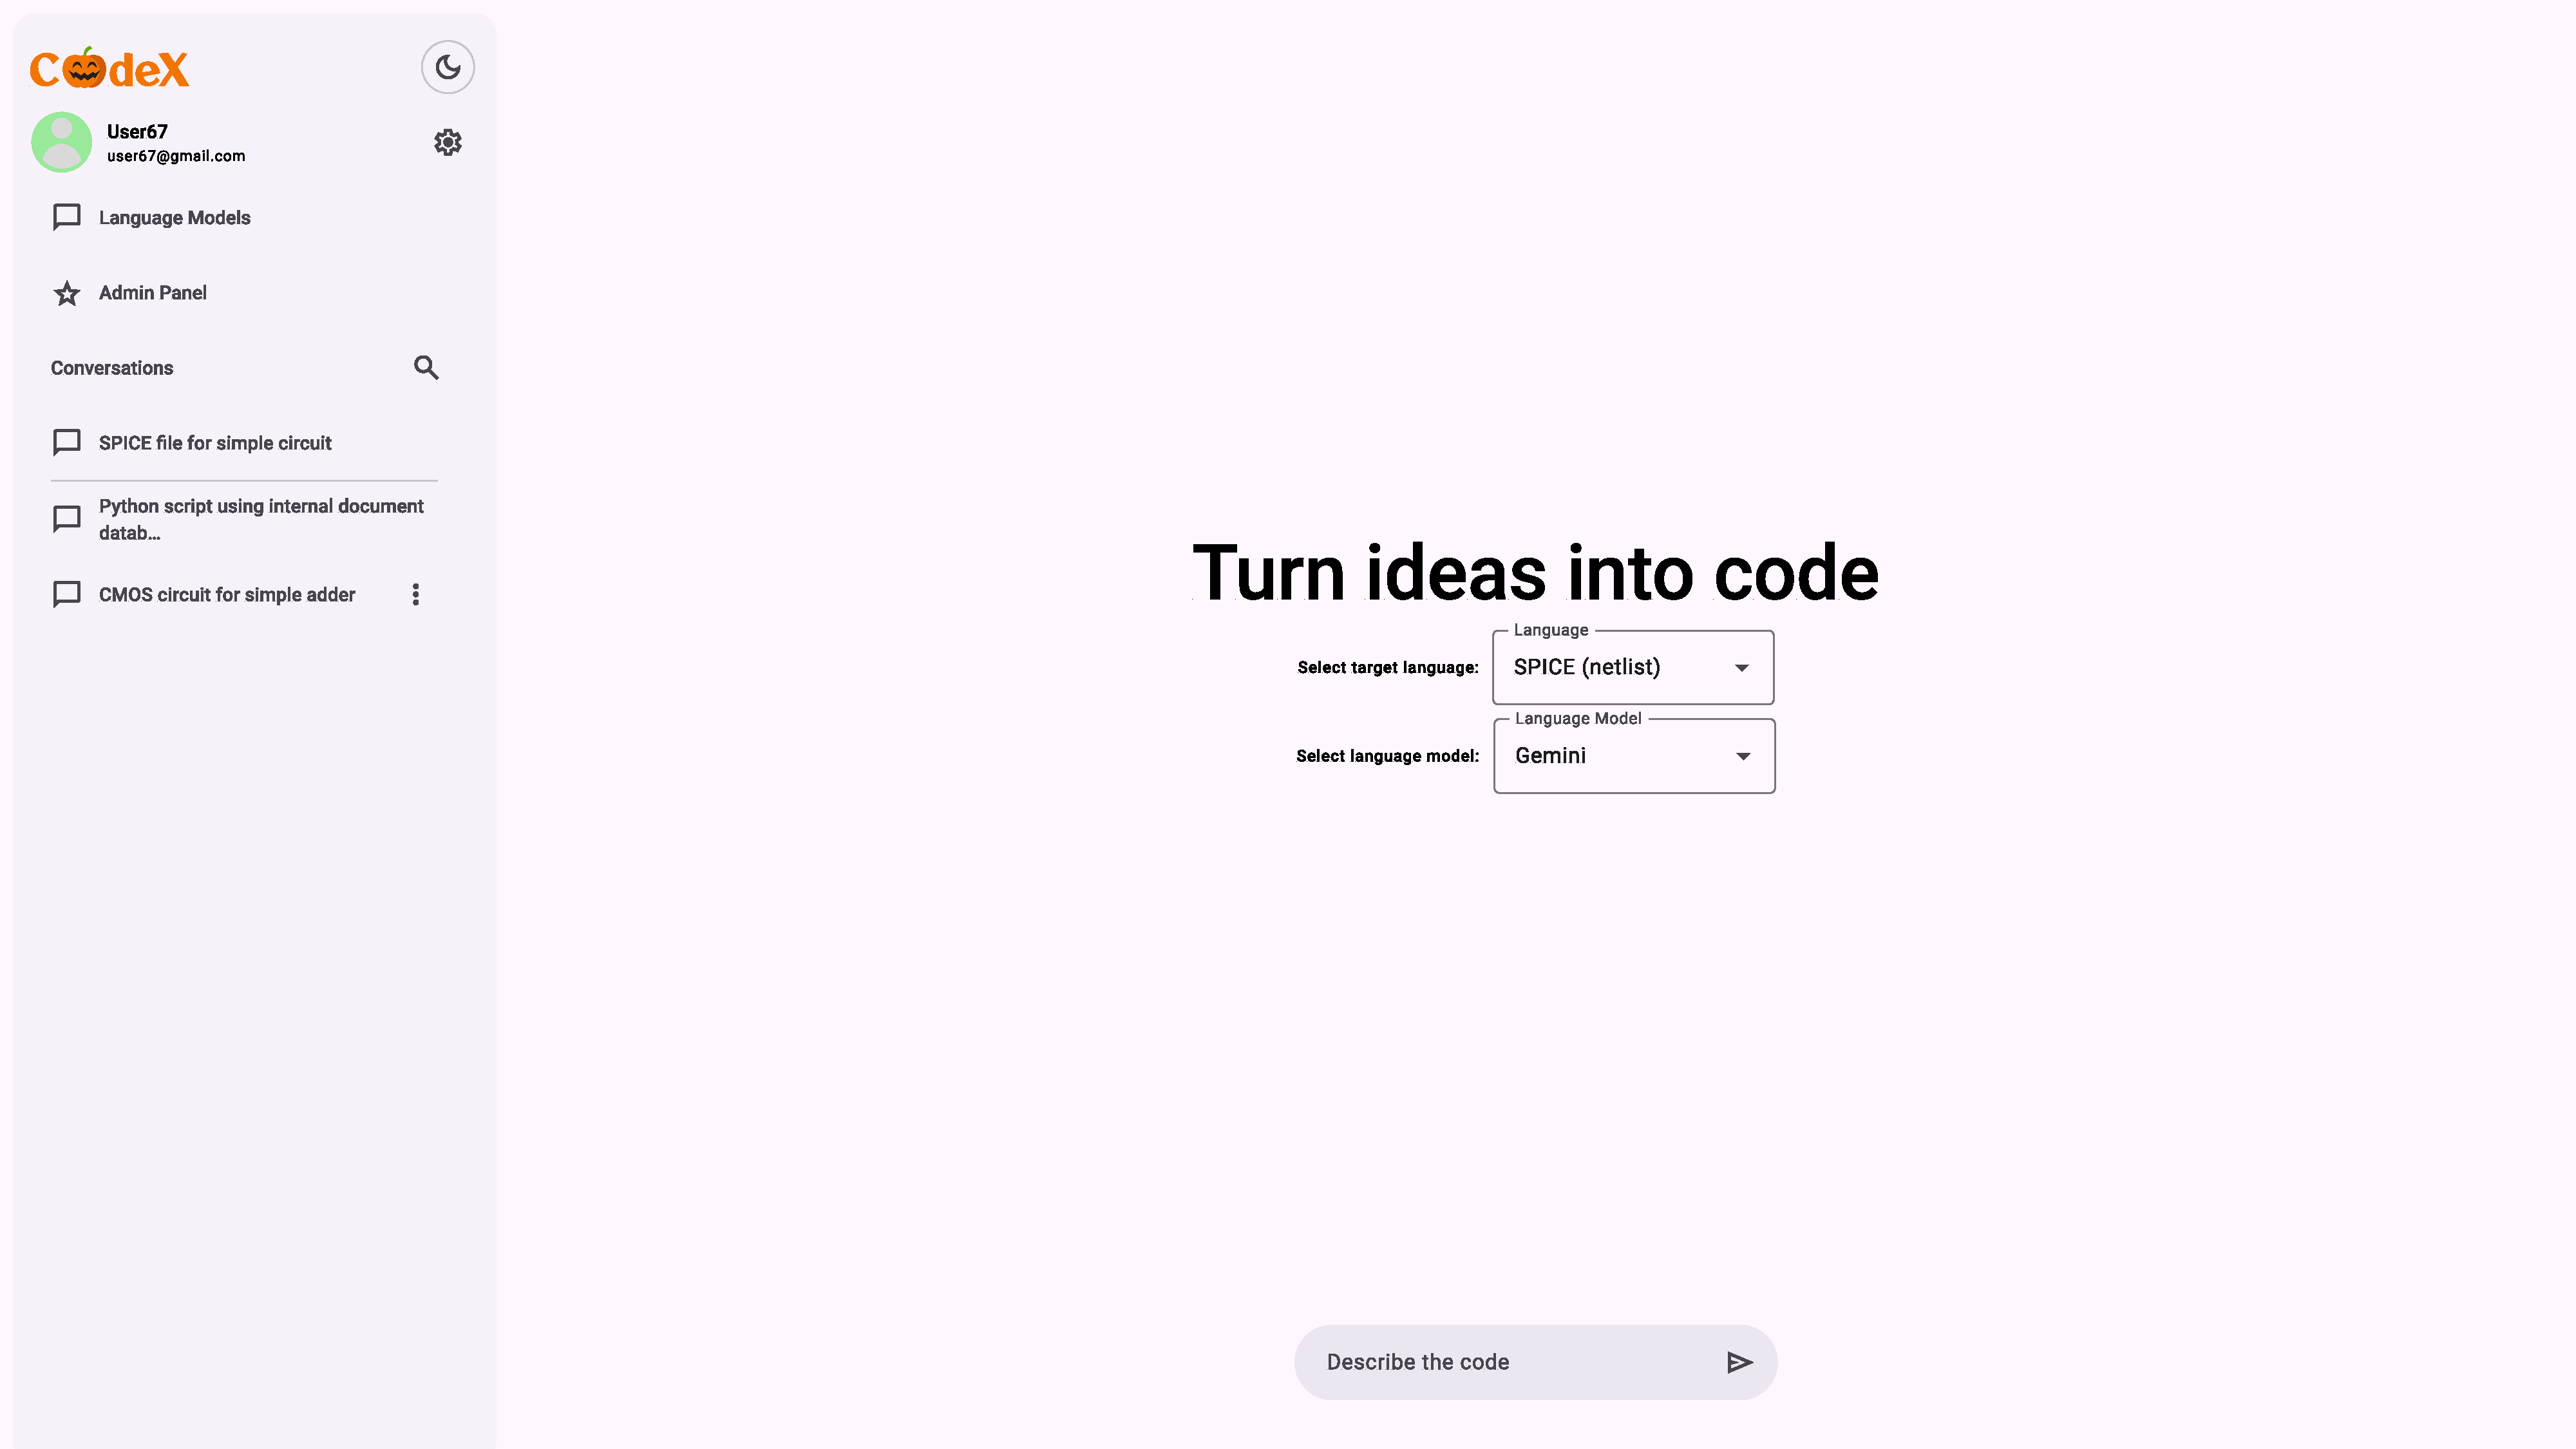
\includegraphics[width=\linewidth]{figures/ui/desktop/Conversation_Screen initial}
    \caption{\hyperref[abr:GUI]{GUI}: Conversation screen before request}
    \label{fig:ui_d_conversation_screen_initial}
\end{figure}
\begin{figure}
    \centering
    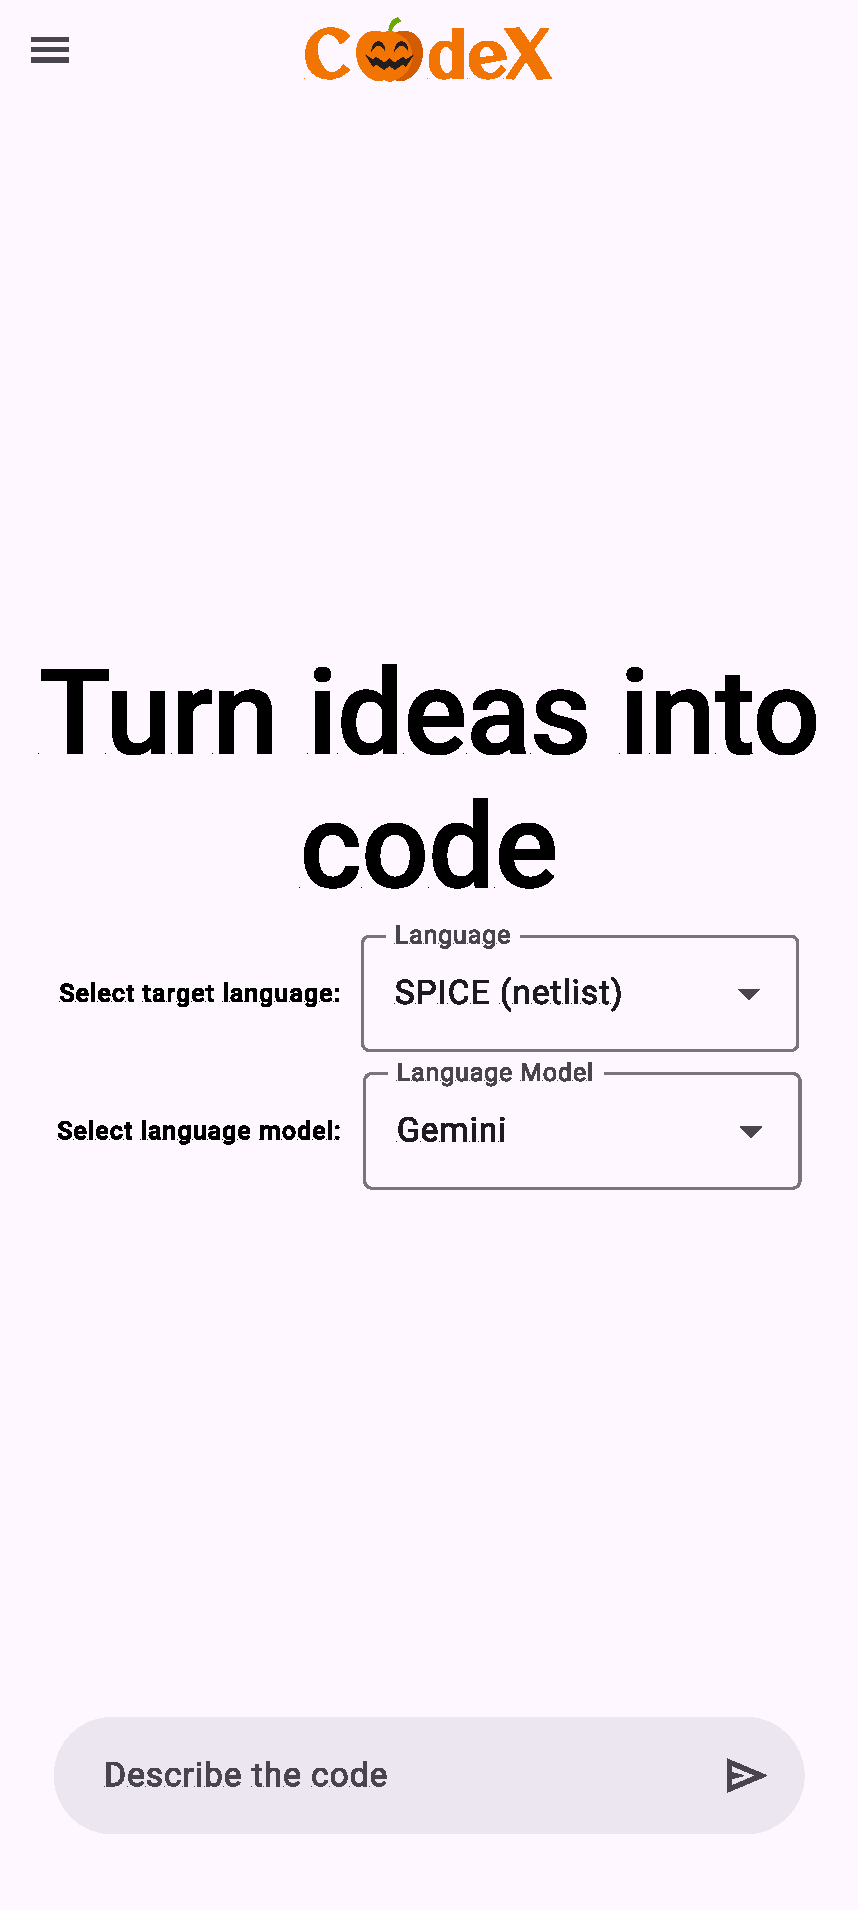
\includegraphics[width=5cm]{figures/ui/mobile/Conversation_Screen initial}
    \caption{\hyperref[abr:GUI]{GUI}: Conversation screen before request (mobile)}
    \label{fig:ui_m_conversation_screen_initial}
\end{figure}

\begin{figure}
    \centering
    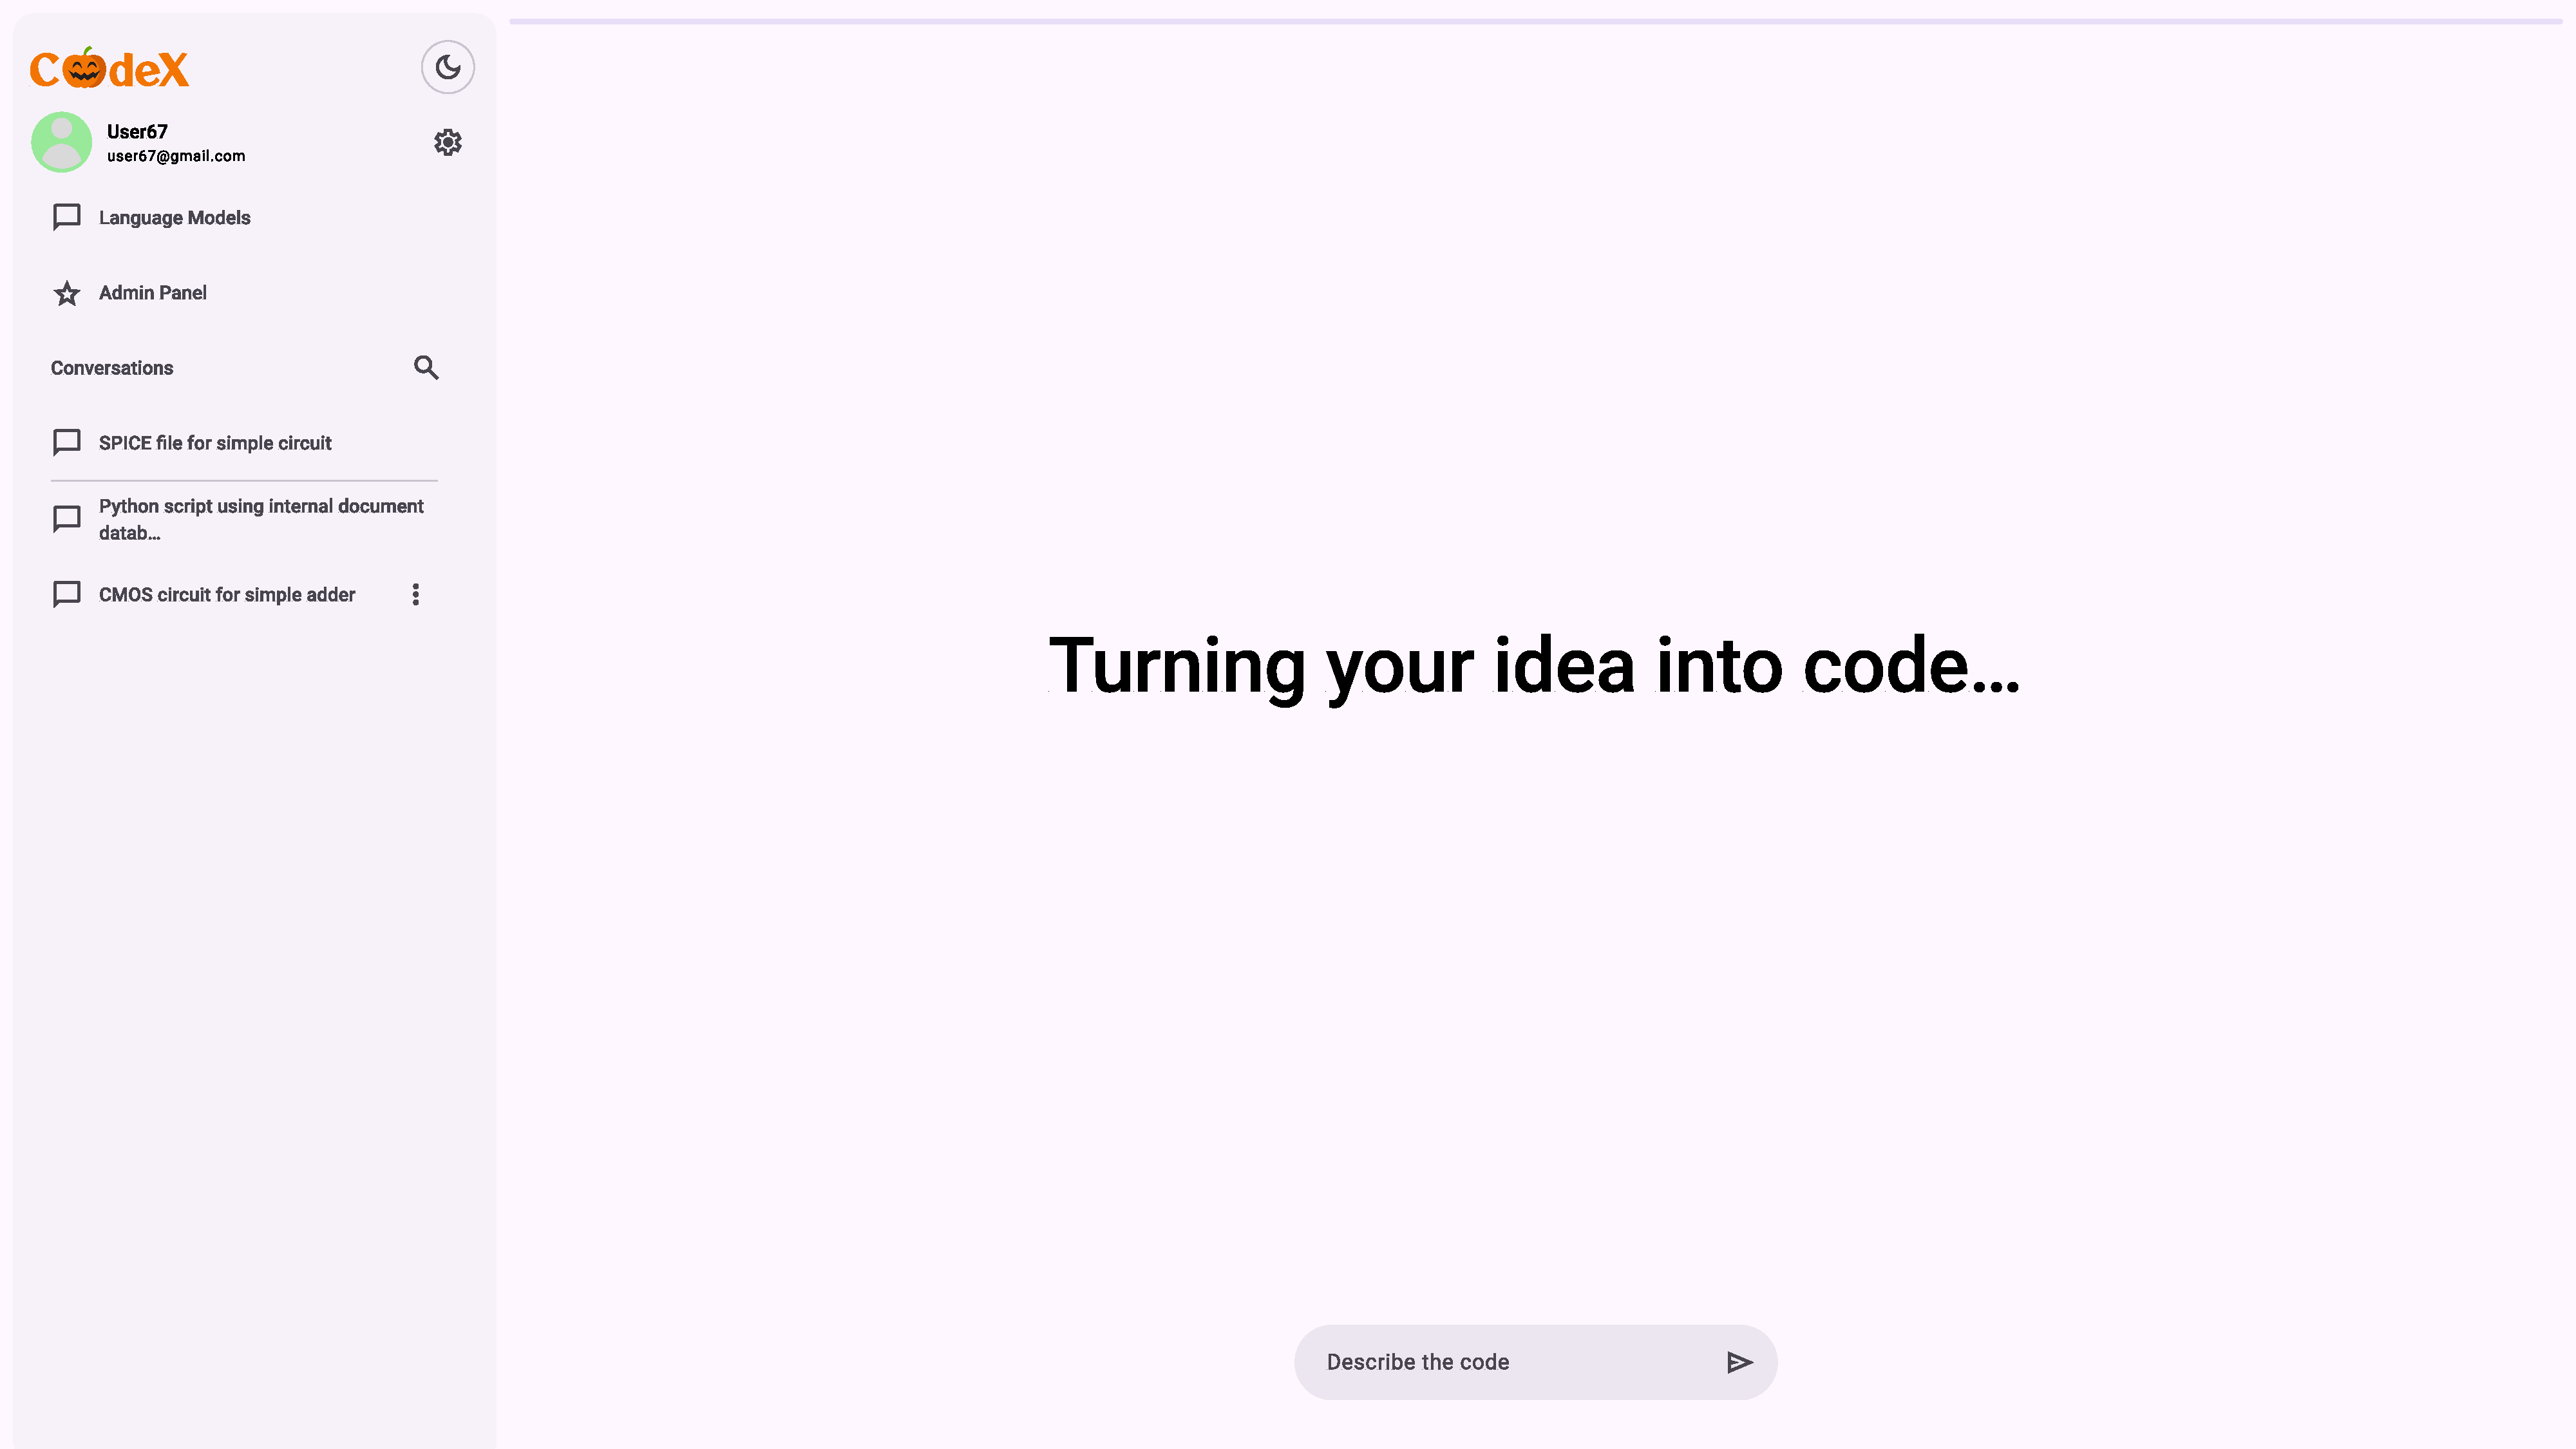
\includegraphics[width=\linewidth]{figures/ui/desktop/Conversation_Screen loading}
    \caption{\hyperref[abr:GUI]{GUI}: Conversation screen during request}
    \label{fig:ui_d_conversation_screen_loading}
\end{figure}
\begin{figure}
    \centering
    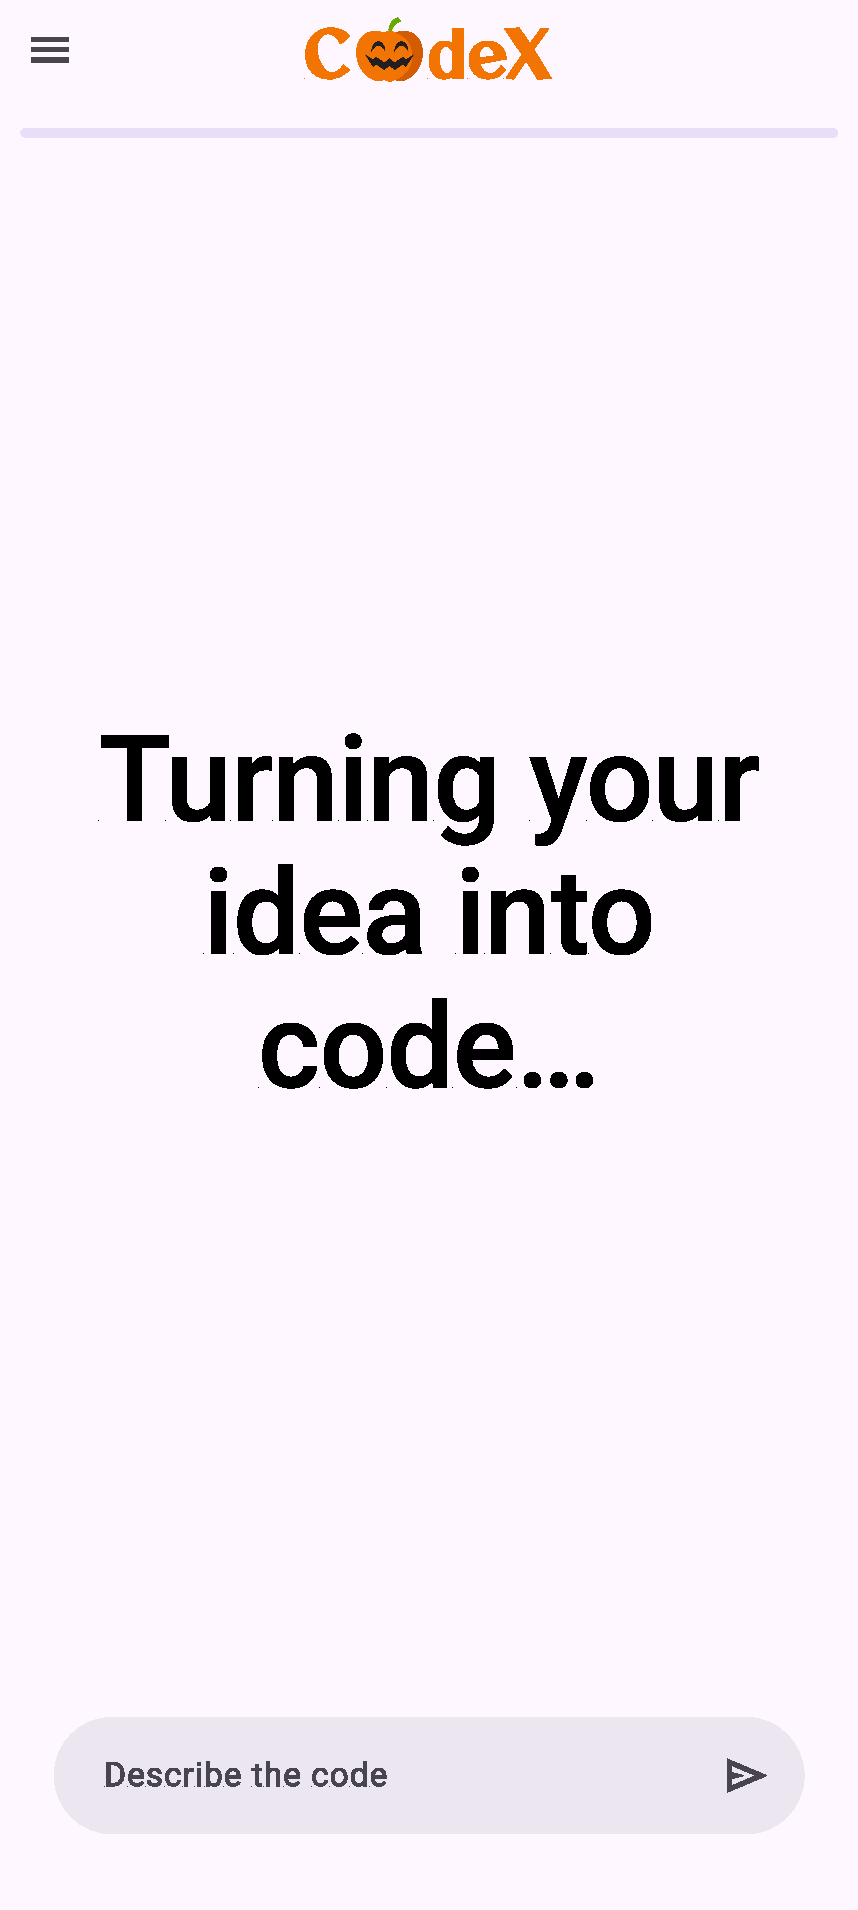
\includegraphics[width=5cm]{figures/ui/mobile/Conversation_Screen loading}
    \caption{\hyperref[abr:GUI]{GUI}: Conversation screen during request (mobile)}
    \label{fig:ui_m_conversation_screen_loading}
\end{figure}

\begin{figure}
    \centering
    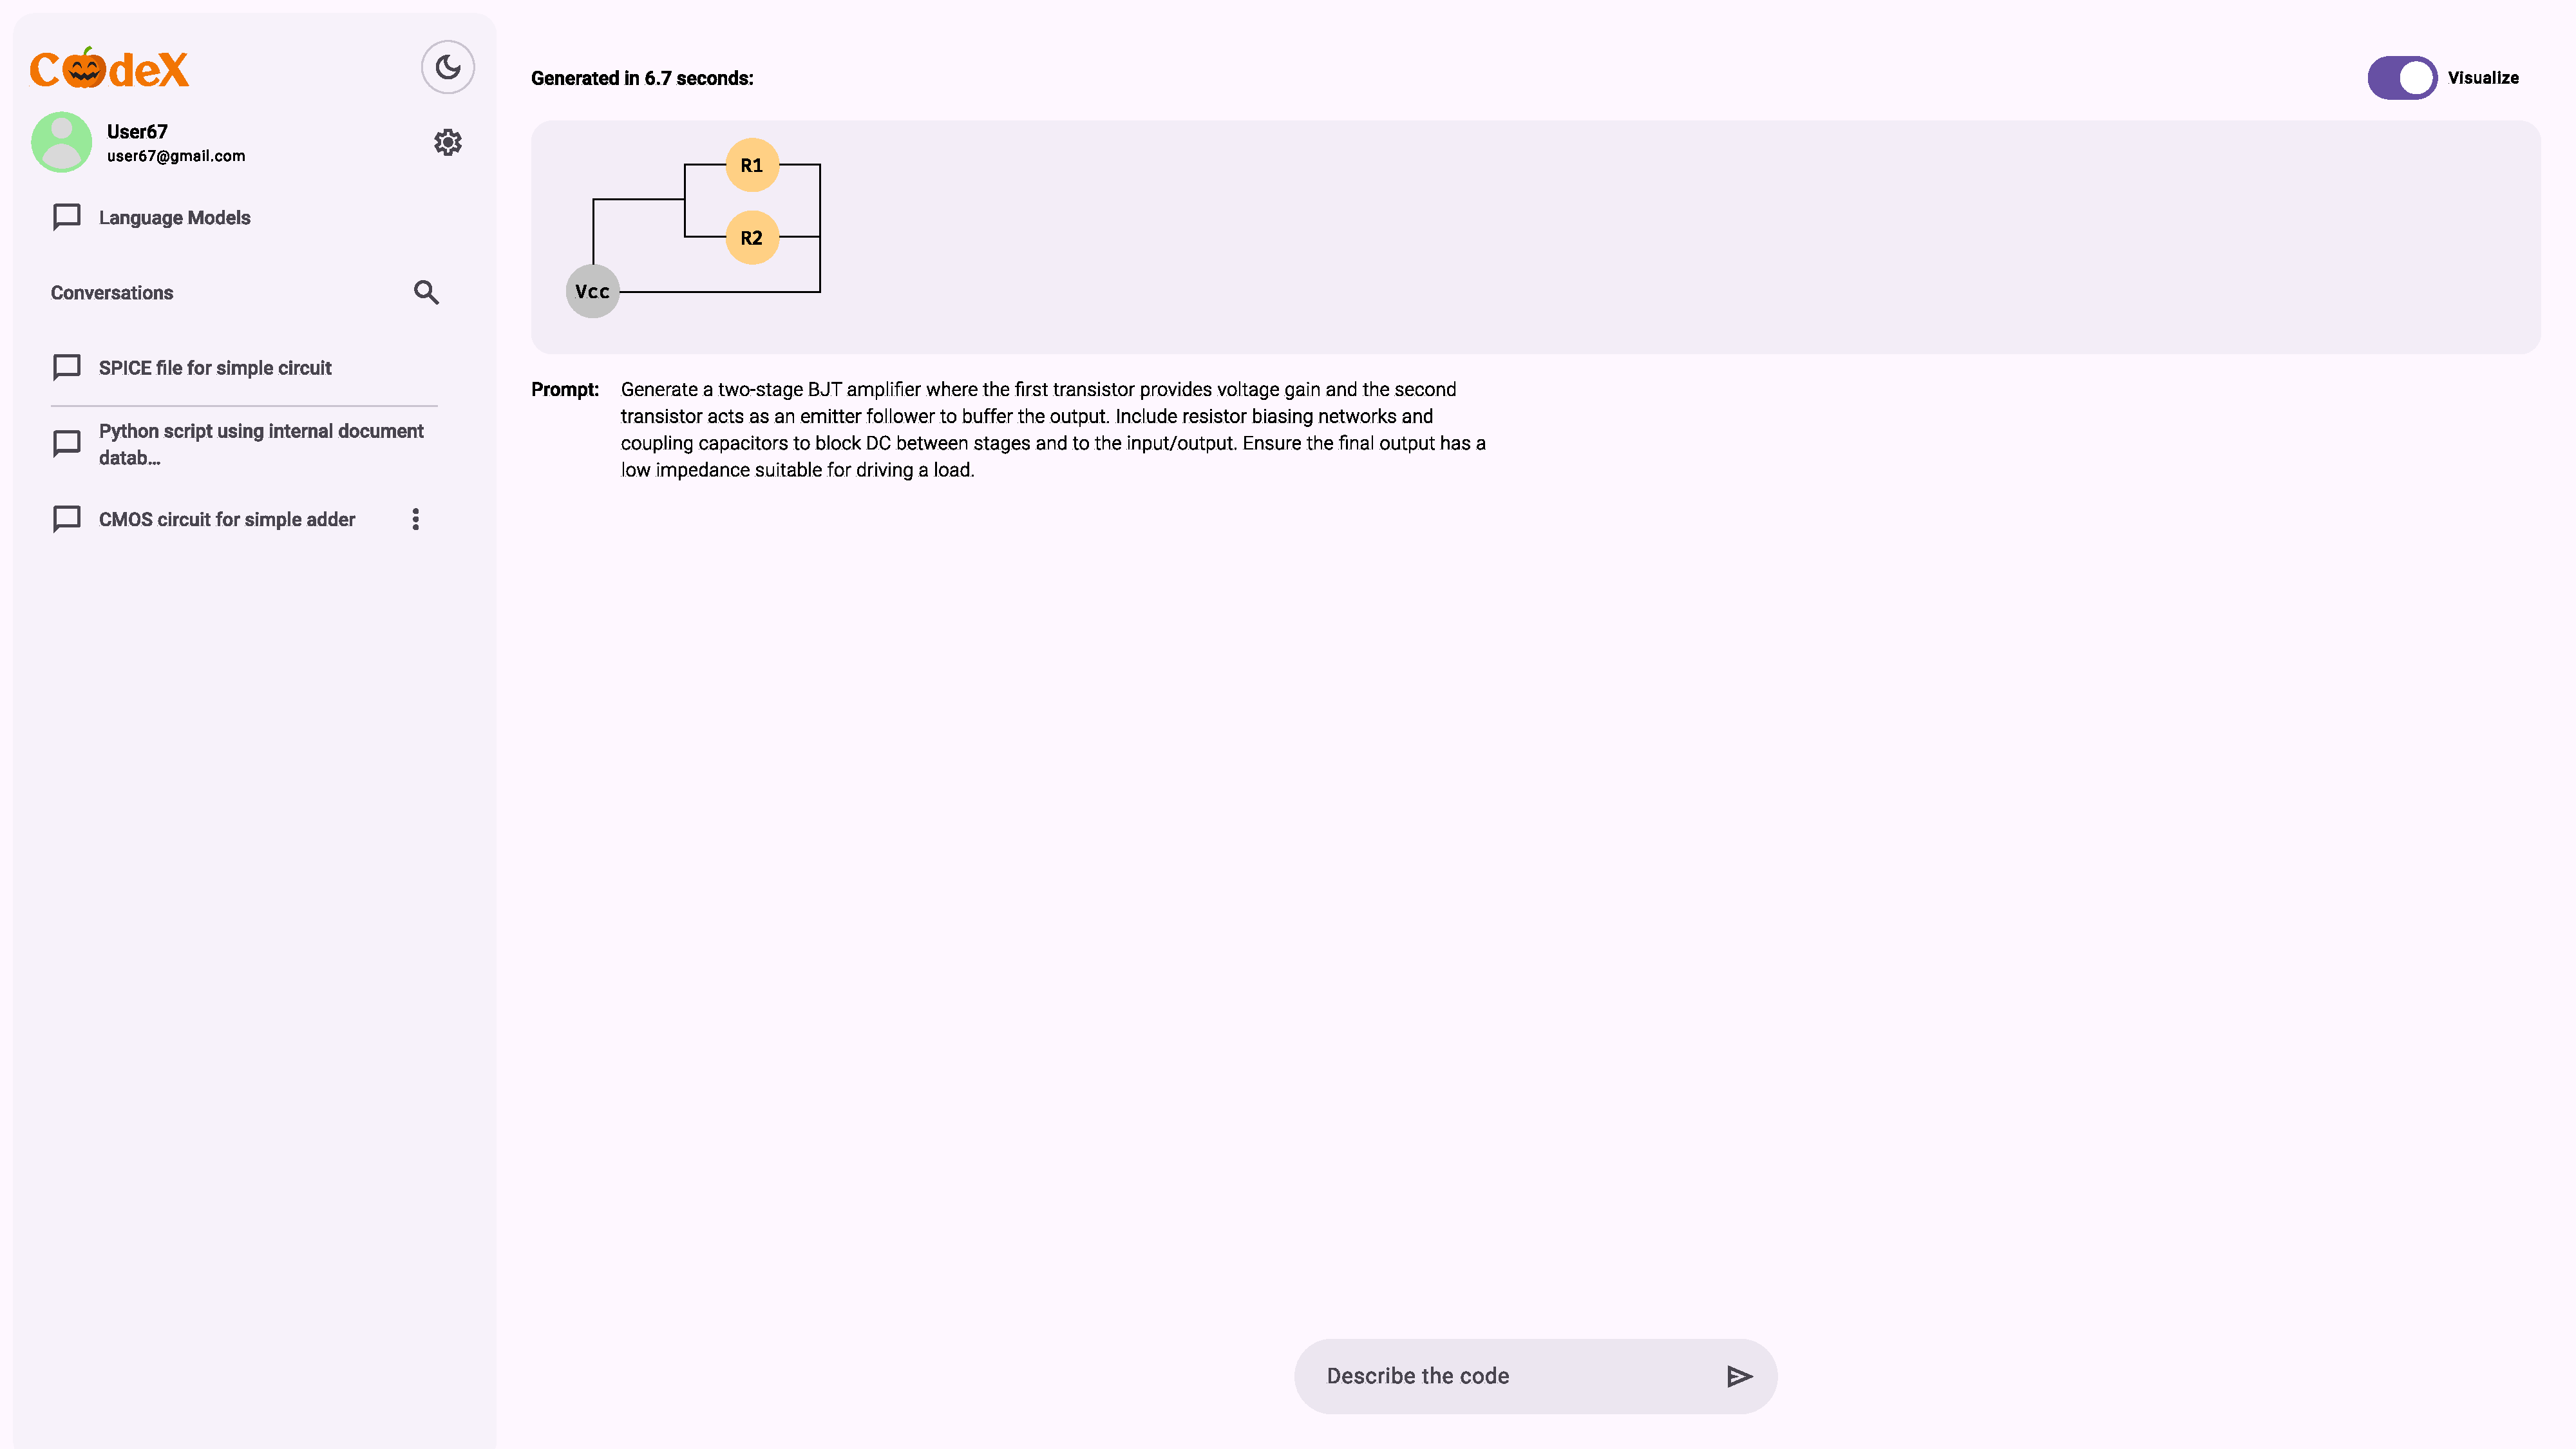
\includegraphics[width=\linewidth]{figures/ui/desktop/Conversation_Screen visualized}
    \caption{\hyperref[abr:GUI]{GUI}: Conversation screen after request with visualization}
    \label{fig:ui_d_conversation_screen_visualized}
\end{figure}
\begin{figure}
    \centering
    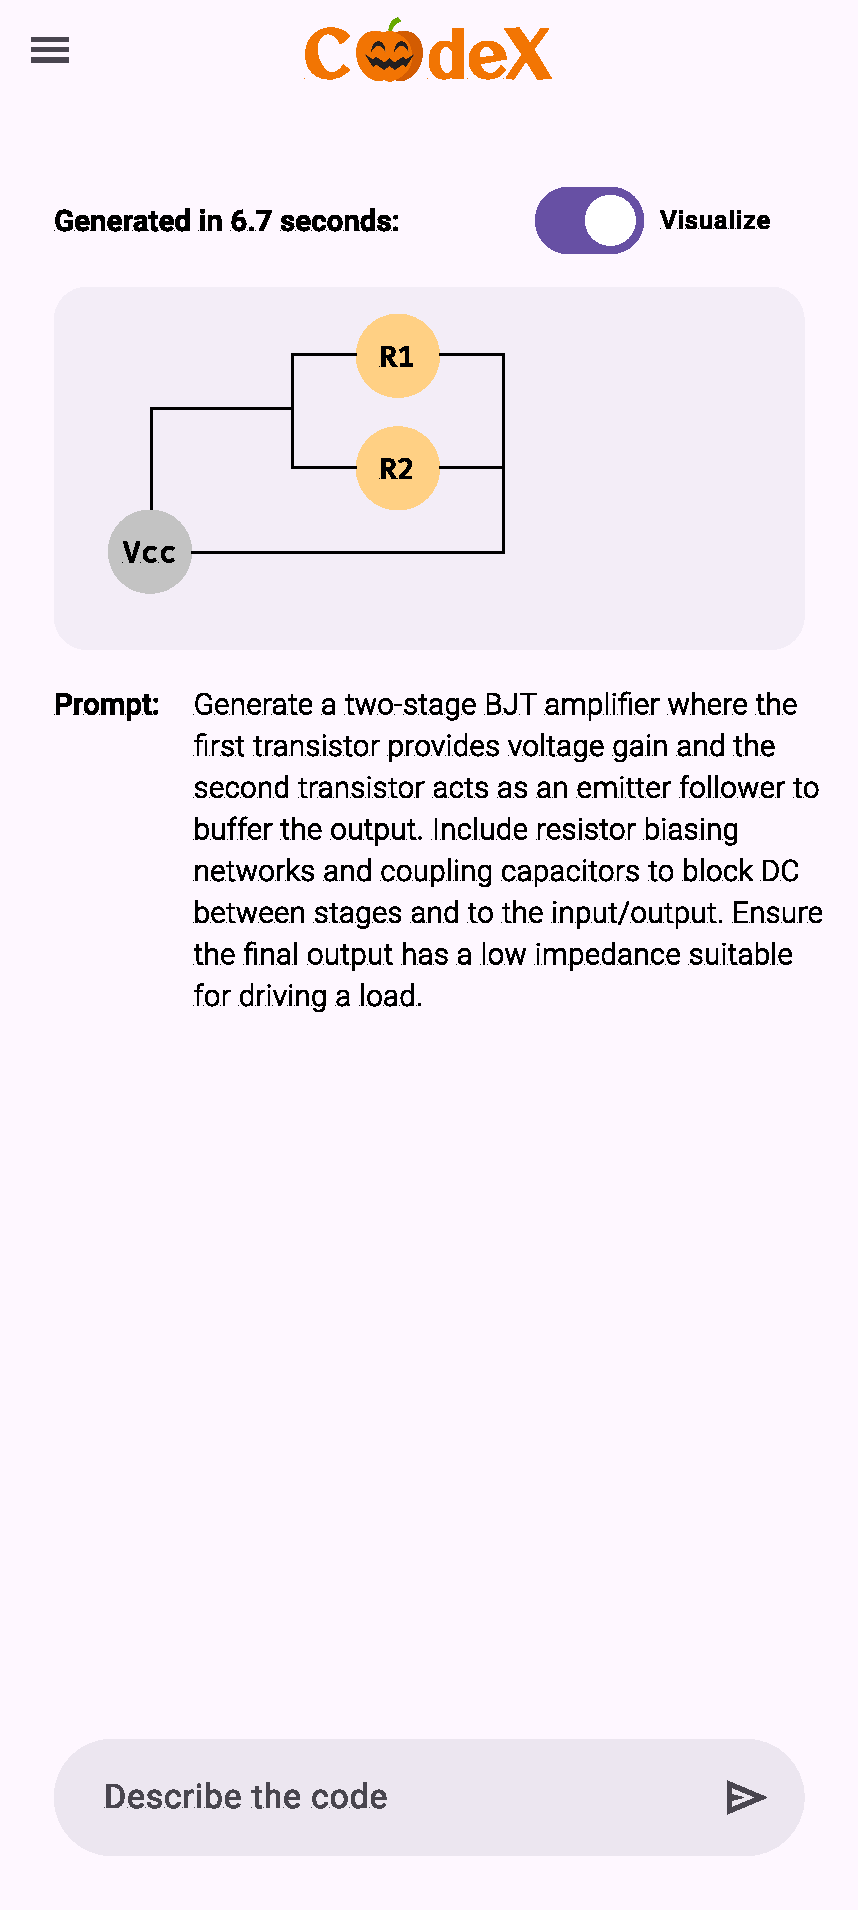
\includegraphics[width=5cm]{figures/ui/mobile/Conversation_Screen visualized}
    \caption{\hyperref[abr:GUI]{GUI}: Conversation screen after request with visualization (mobile)}
    \label{fig:ui_m_conversation_screen_visualized}
\end{figure}

\begin{figure}
    \centering
    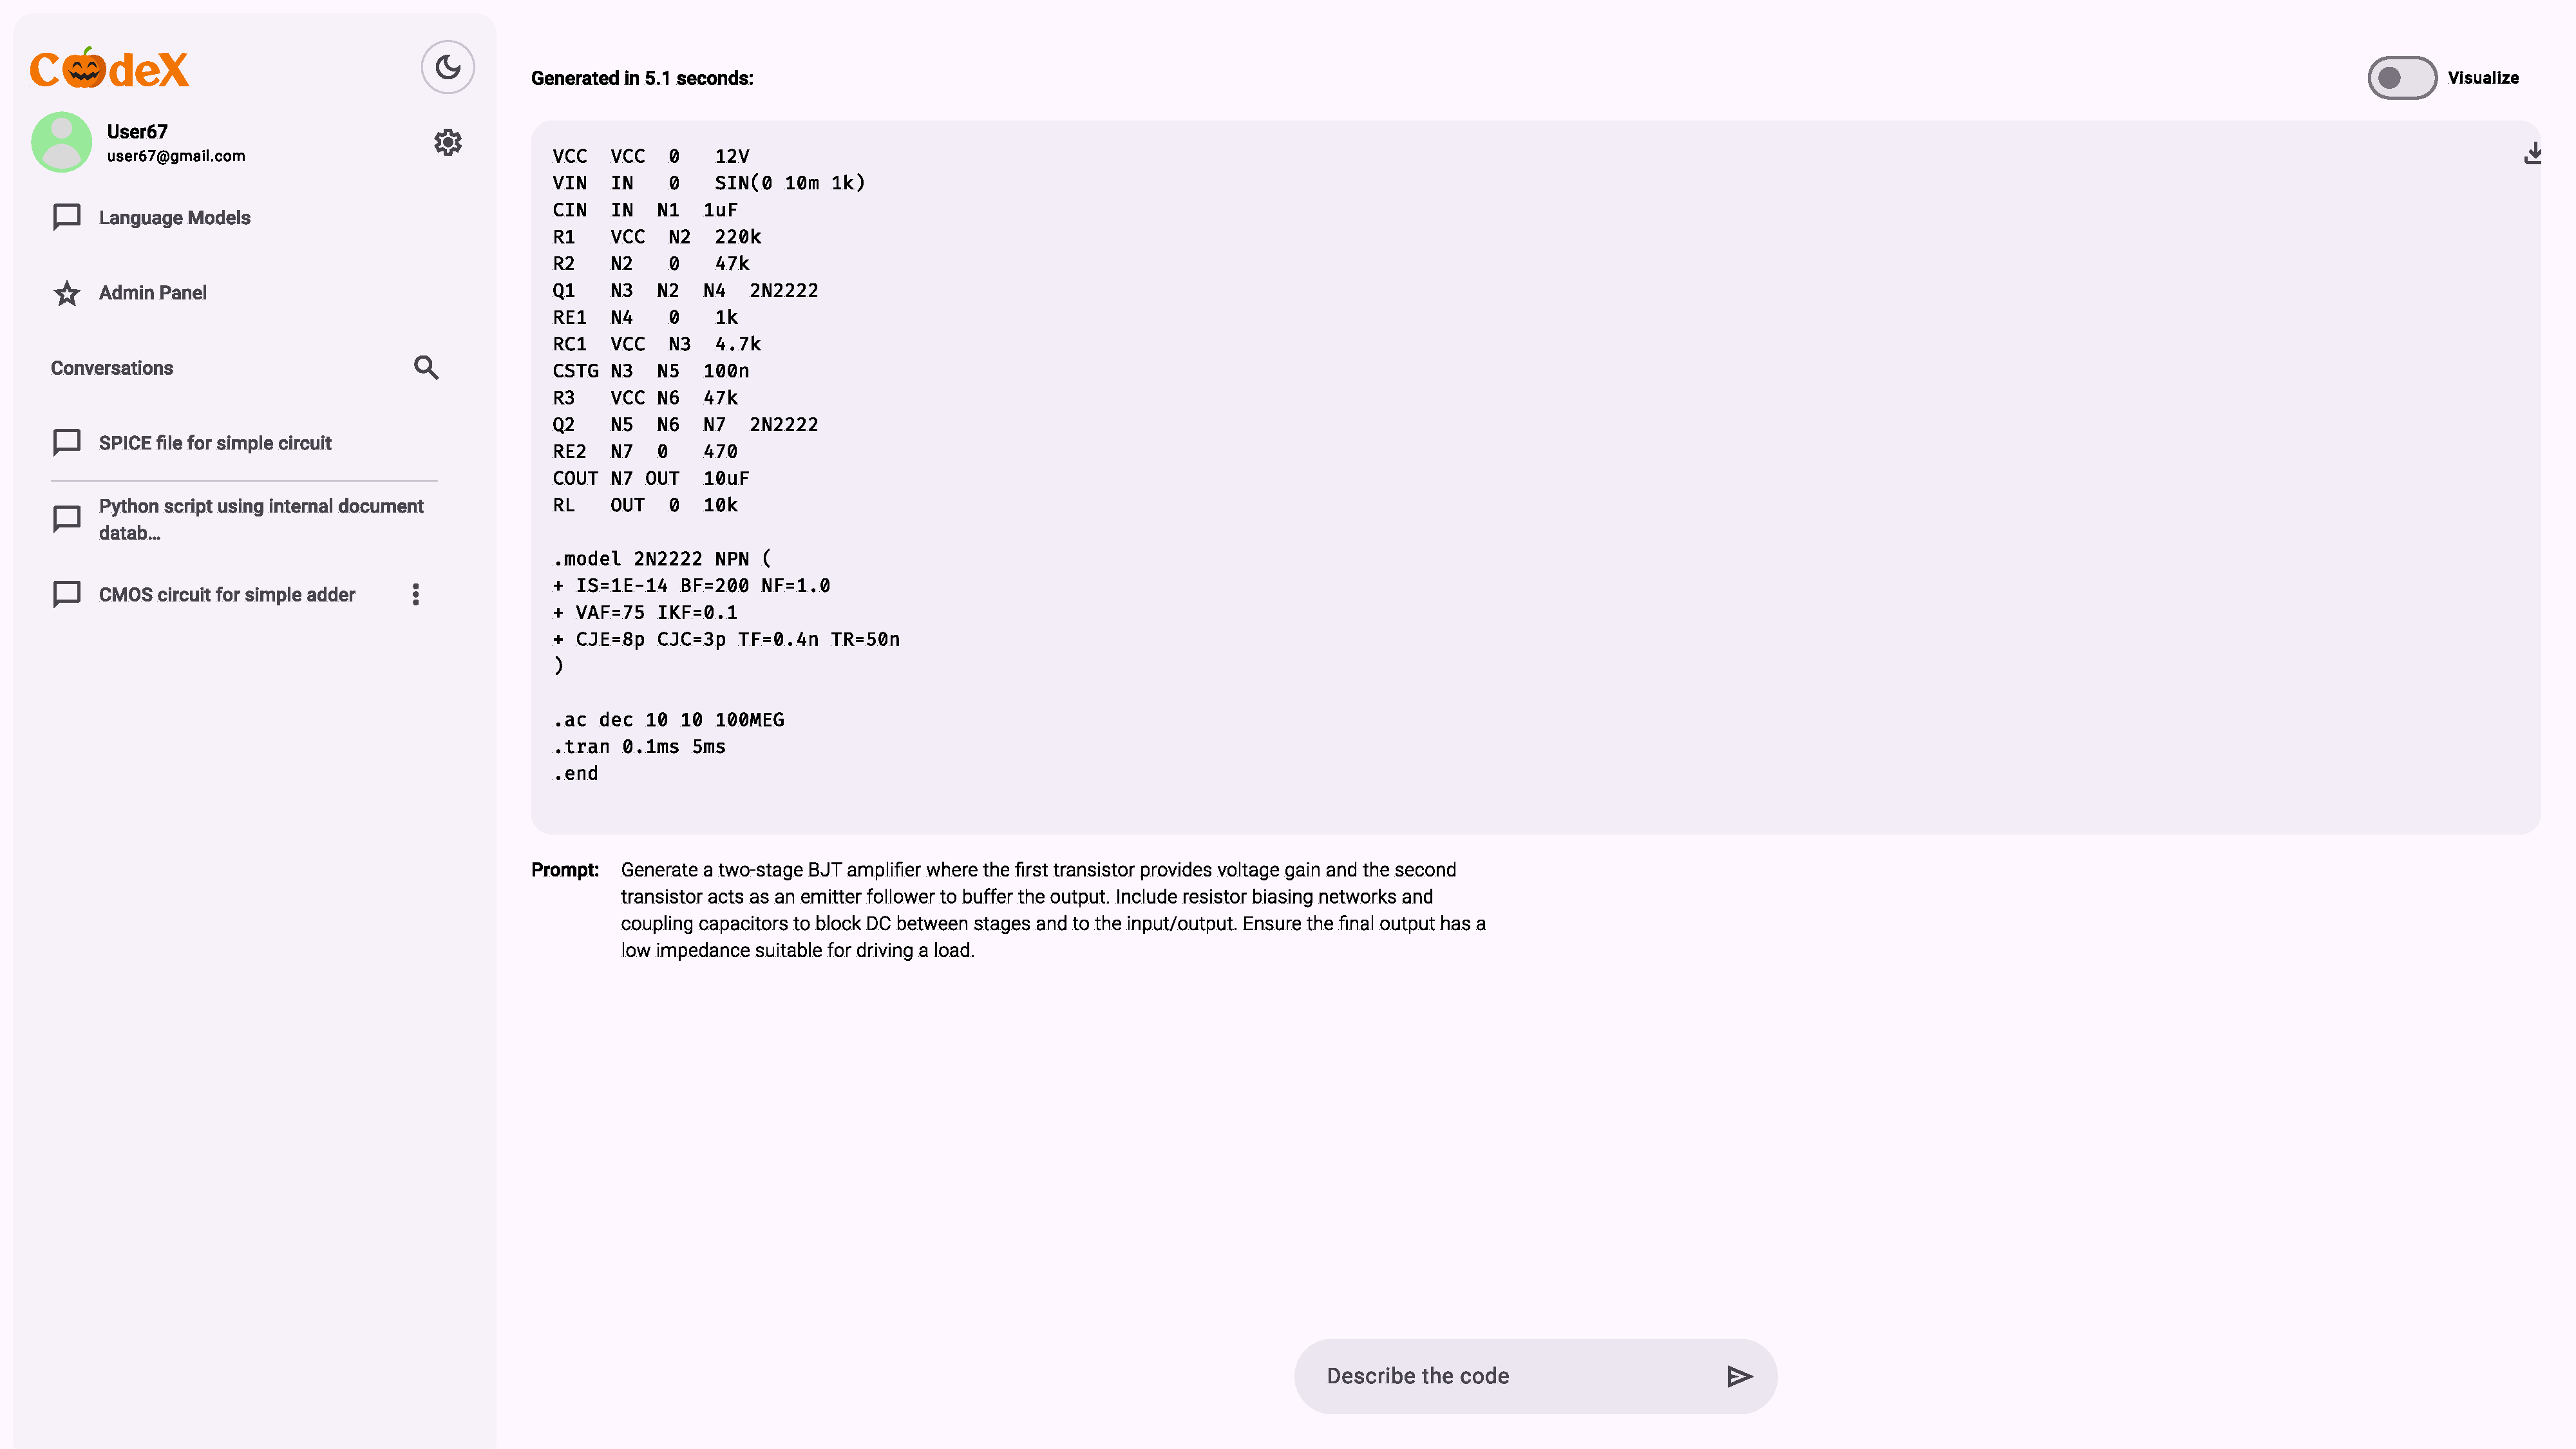
\includegraphics[width=\linewidth]{figures/ui/desktop/Conversation_Screen not-visualized}
    \caption{\hyperref[abr:GUI]{GUI}: Conversation screen after request without visualization}
    \label{fig:ui_d_conversation_screen_not_visualized}
\end{figure}
\begin{figure}
    \centering
    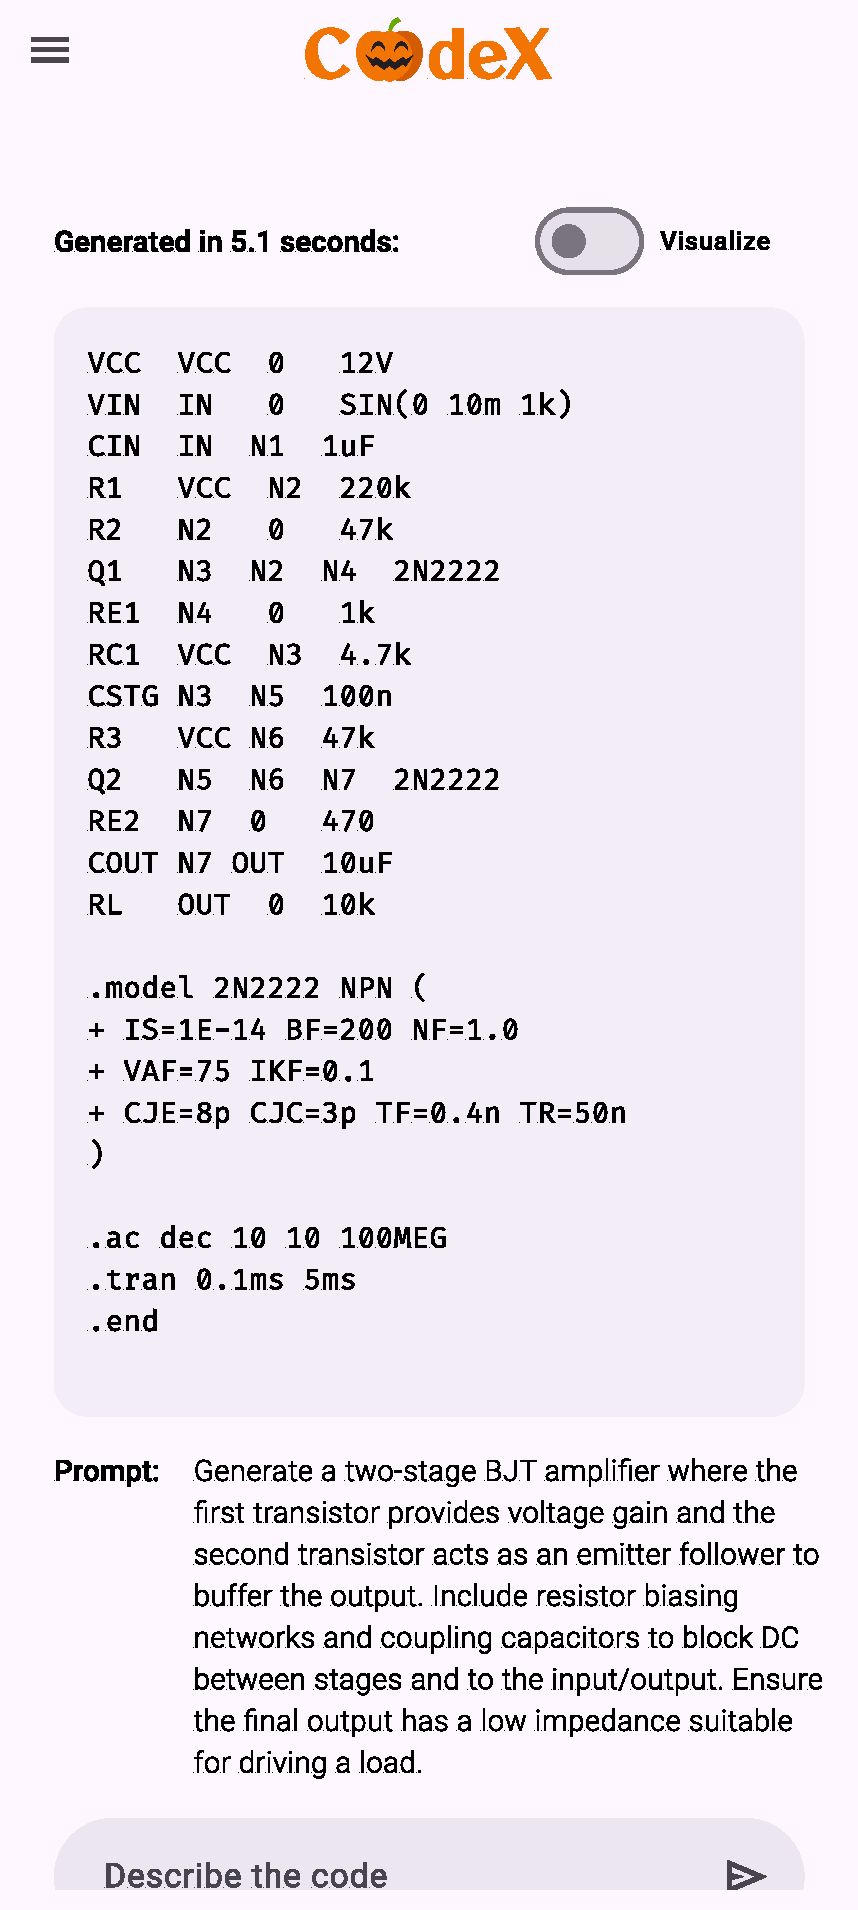
\includegraphics[width=5cm]{figures/ui/mobile/Conversation_Screen not-visualized}
    \caption{\hyperref[abr:GUI]{GUI}: Conversation screen after request without visualization (mobile)}
    \label{fig:ui_m_conversation_screen_not_visualized}
\end{figure}

\subsection{Admin Panel}
The admin panel (\ref{fig:ui-d-admin-panel}/\ref{fig:ui-m-admin-panel}) is where admins can view analytics and update quota settings.
\begin{figure}
    \centering
    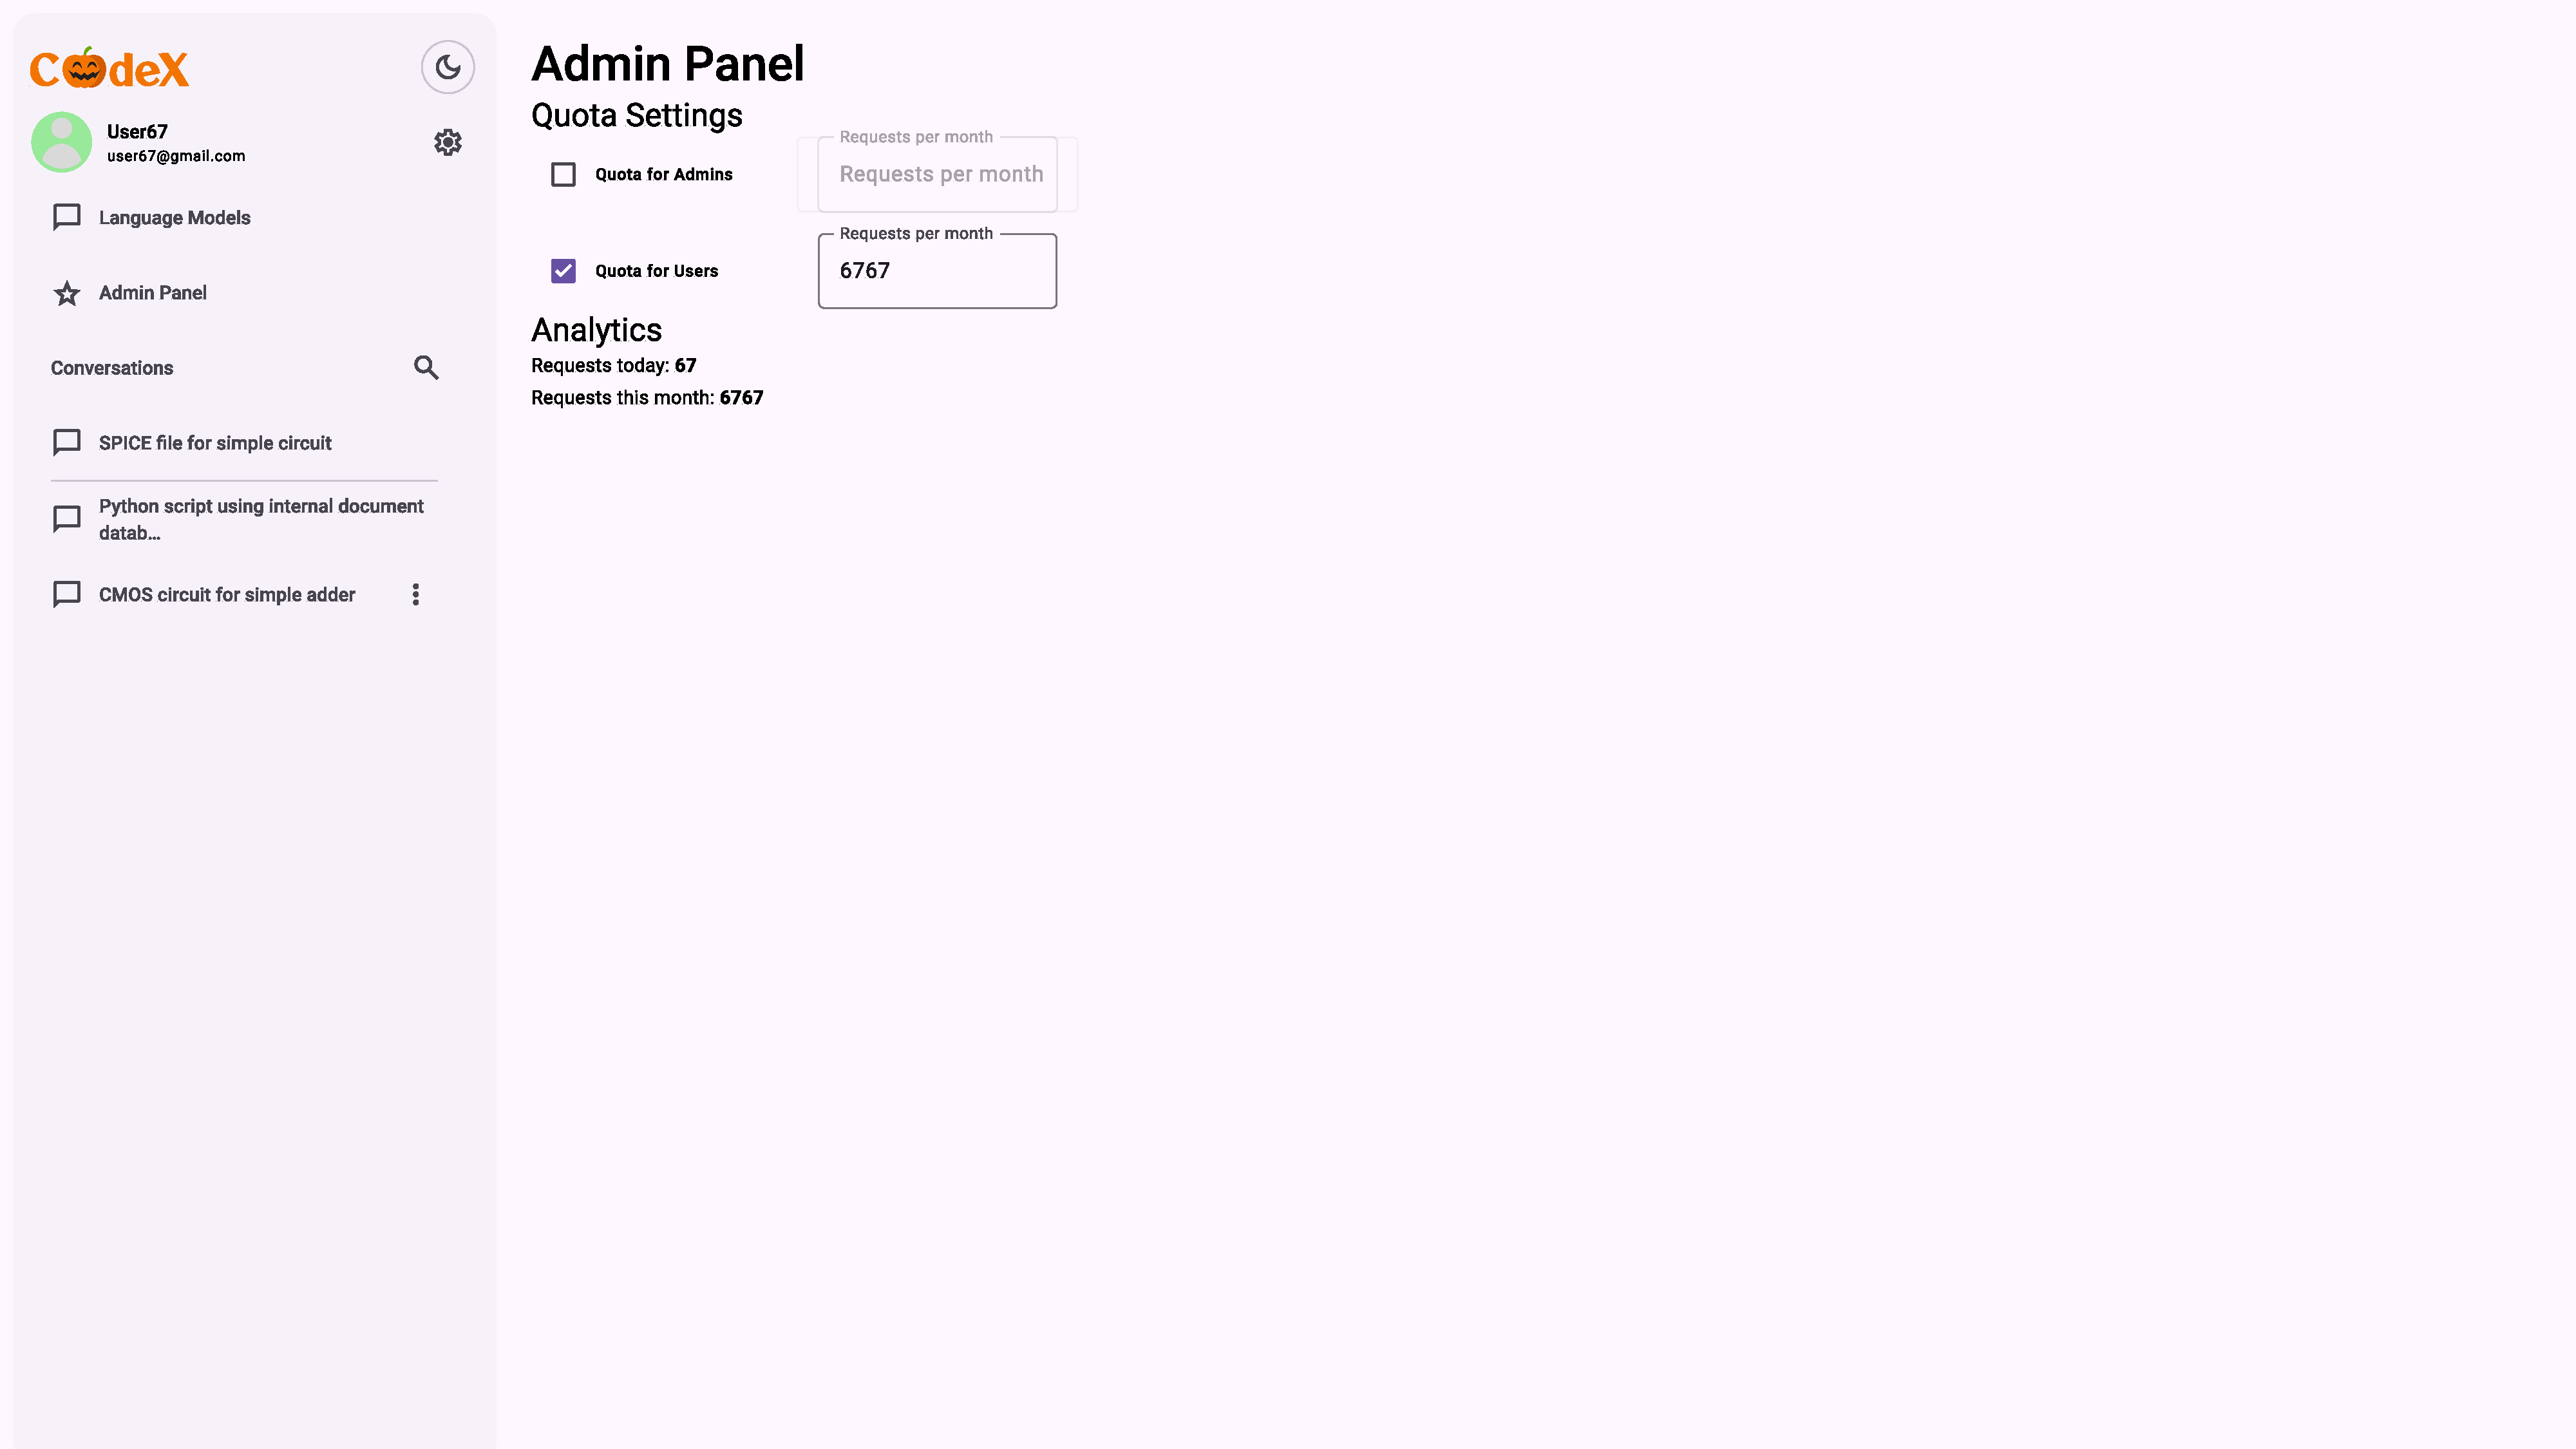
\includegraphics[width=\linewidth]{figures/ui/desktop/Admin_Panel_Screen}
    \caption{\hyperref[abr:GUI]{GUI}: Admin panel}
    \label{fig:ui-d-admin-panel}
\end{figure}
\begin{figure}
    \centering
    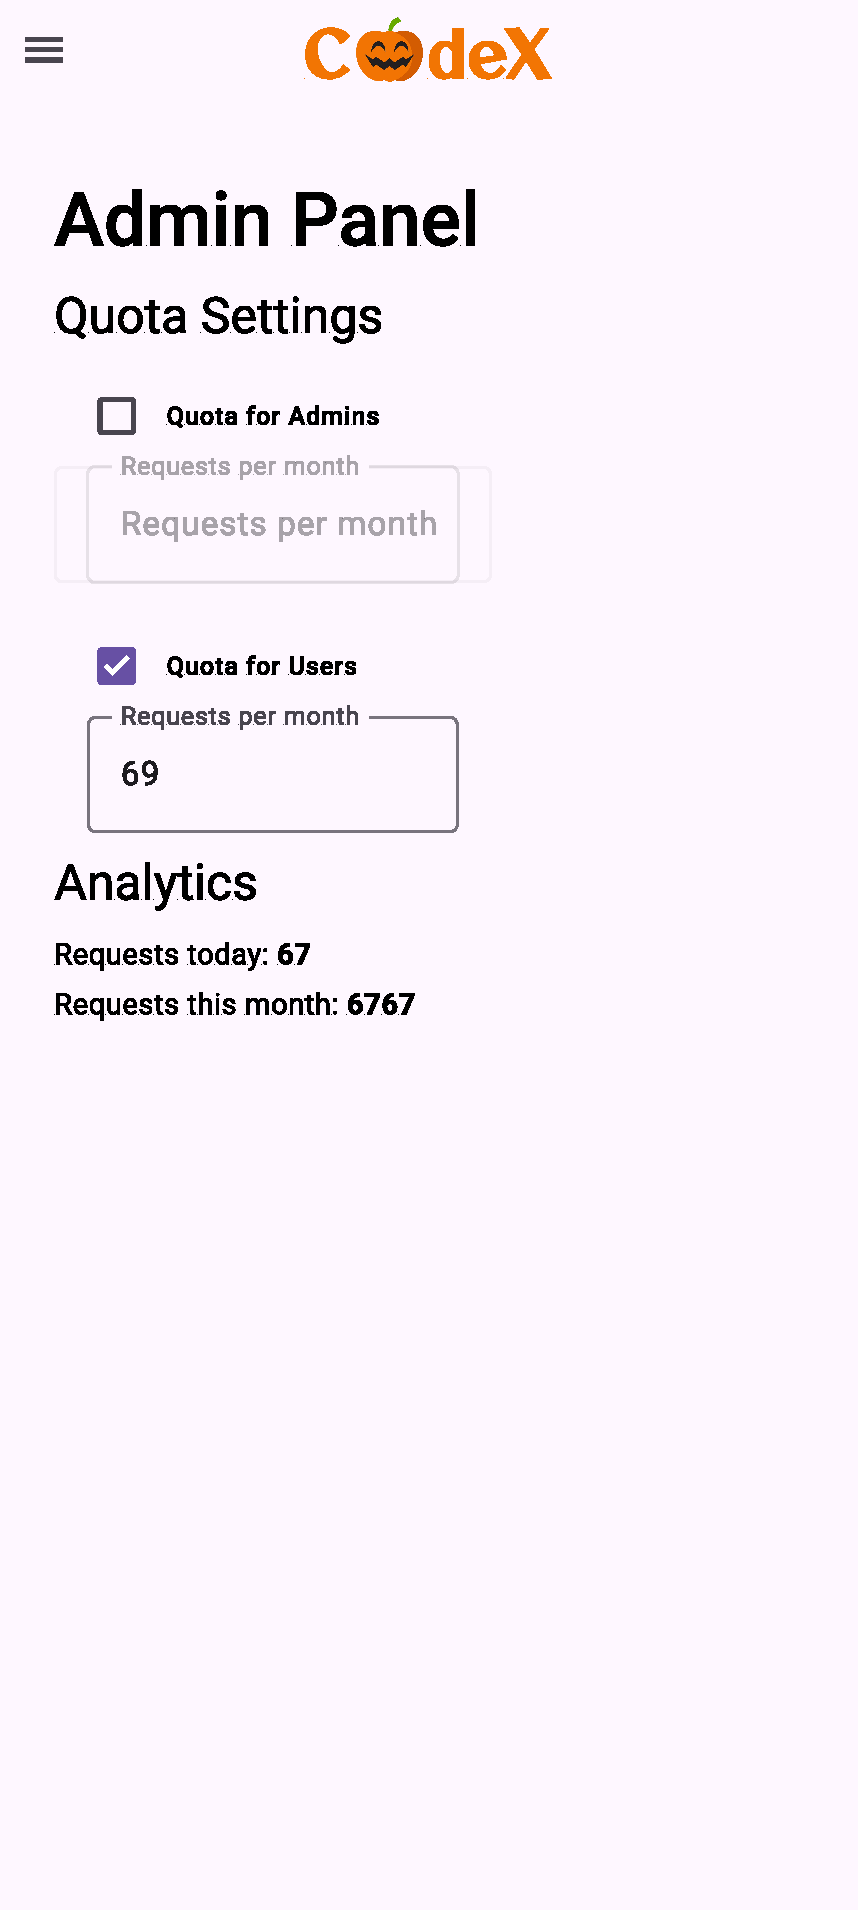
\includegraphics[width=5cm]{figures/ui/mobile/Admin_Panel_Screen}
    \caption{\hyperref[abr:GUI]{GUI}: Admin panel (mobile)}
    \label{fig:ui-m-admin-panel}
\end{figure}

\subsection{Settings}
The settings screen (\ref{fig:ui-d-settings}/\ref{fig:ui-m-settings}) is where the user can add, delete and update LLM-configurations.
\begin{figure}
    \centering
    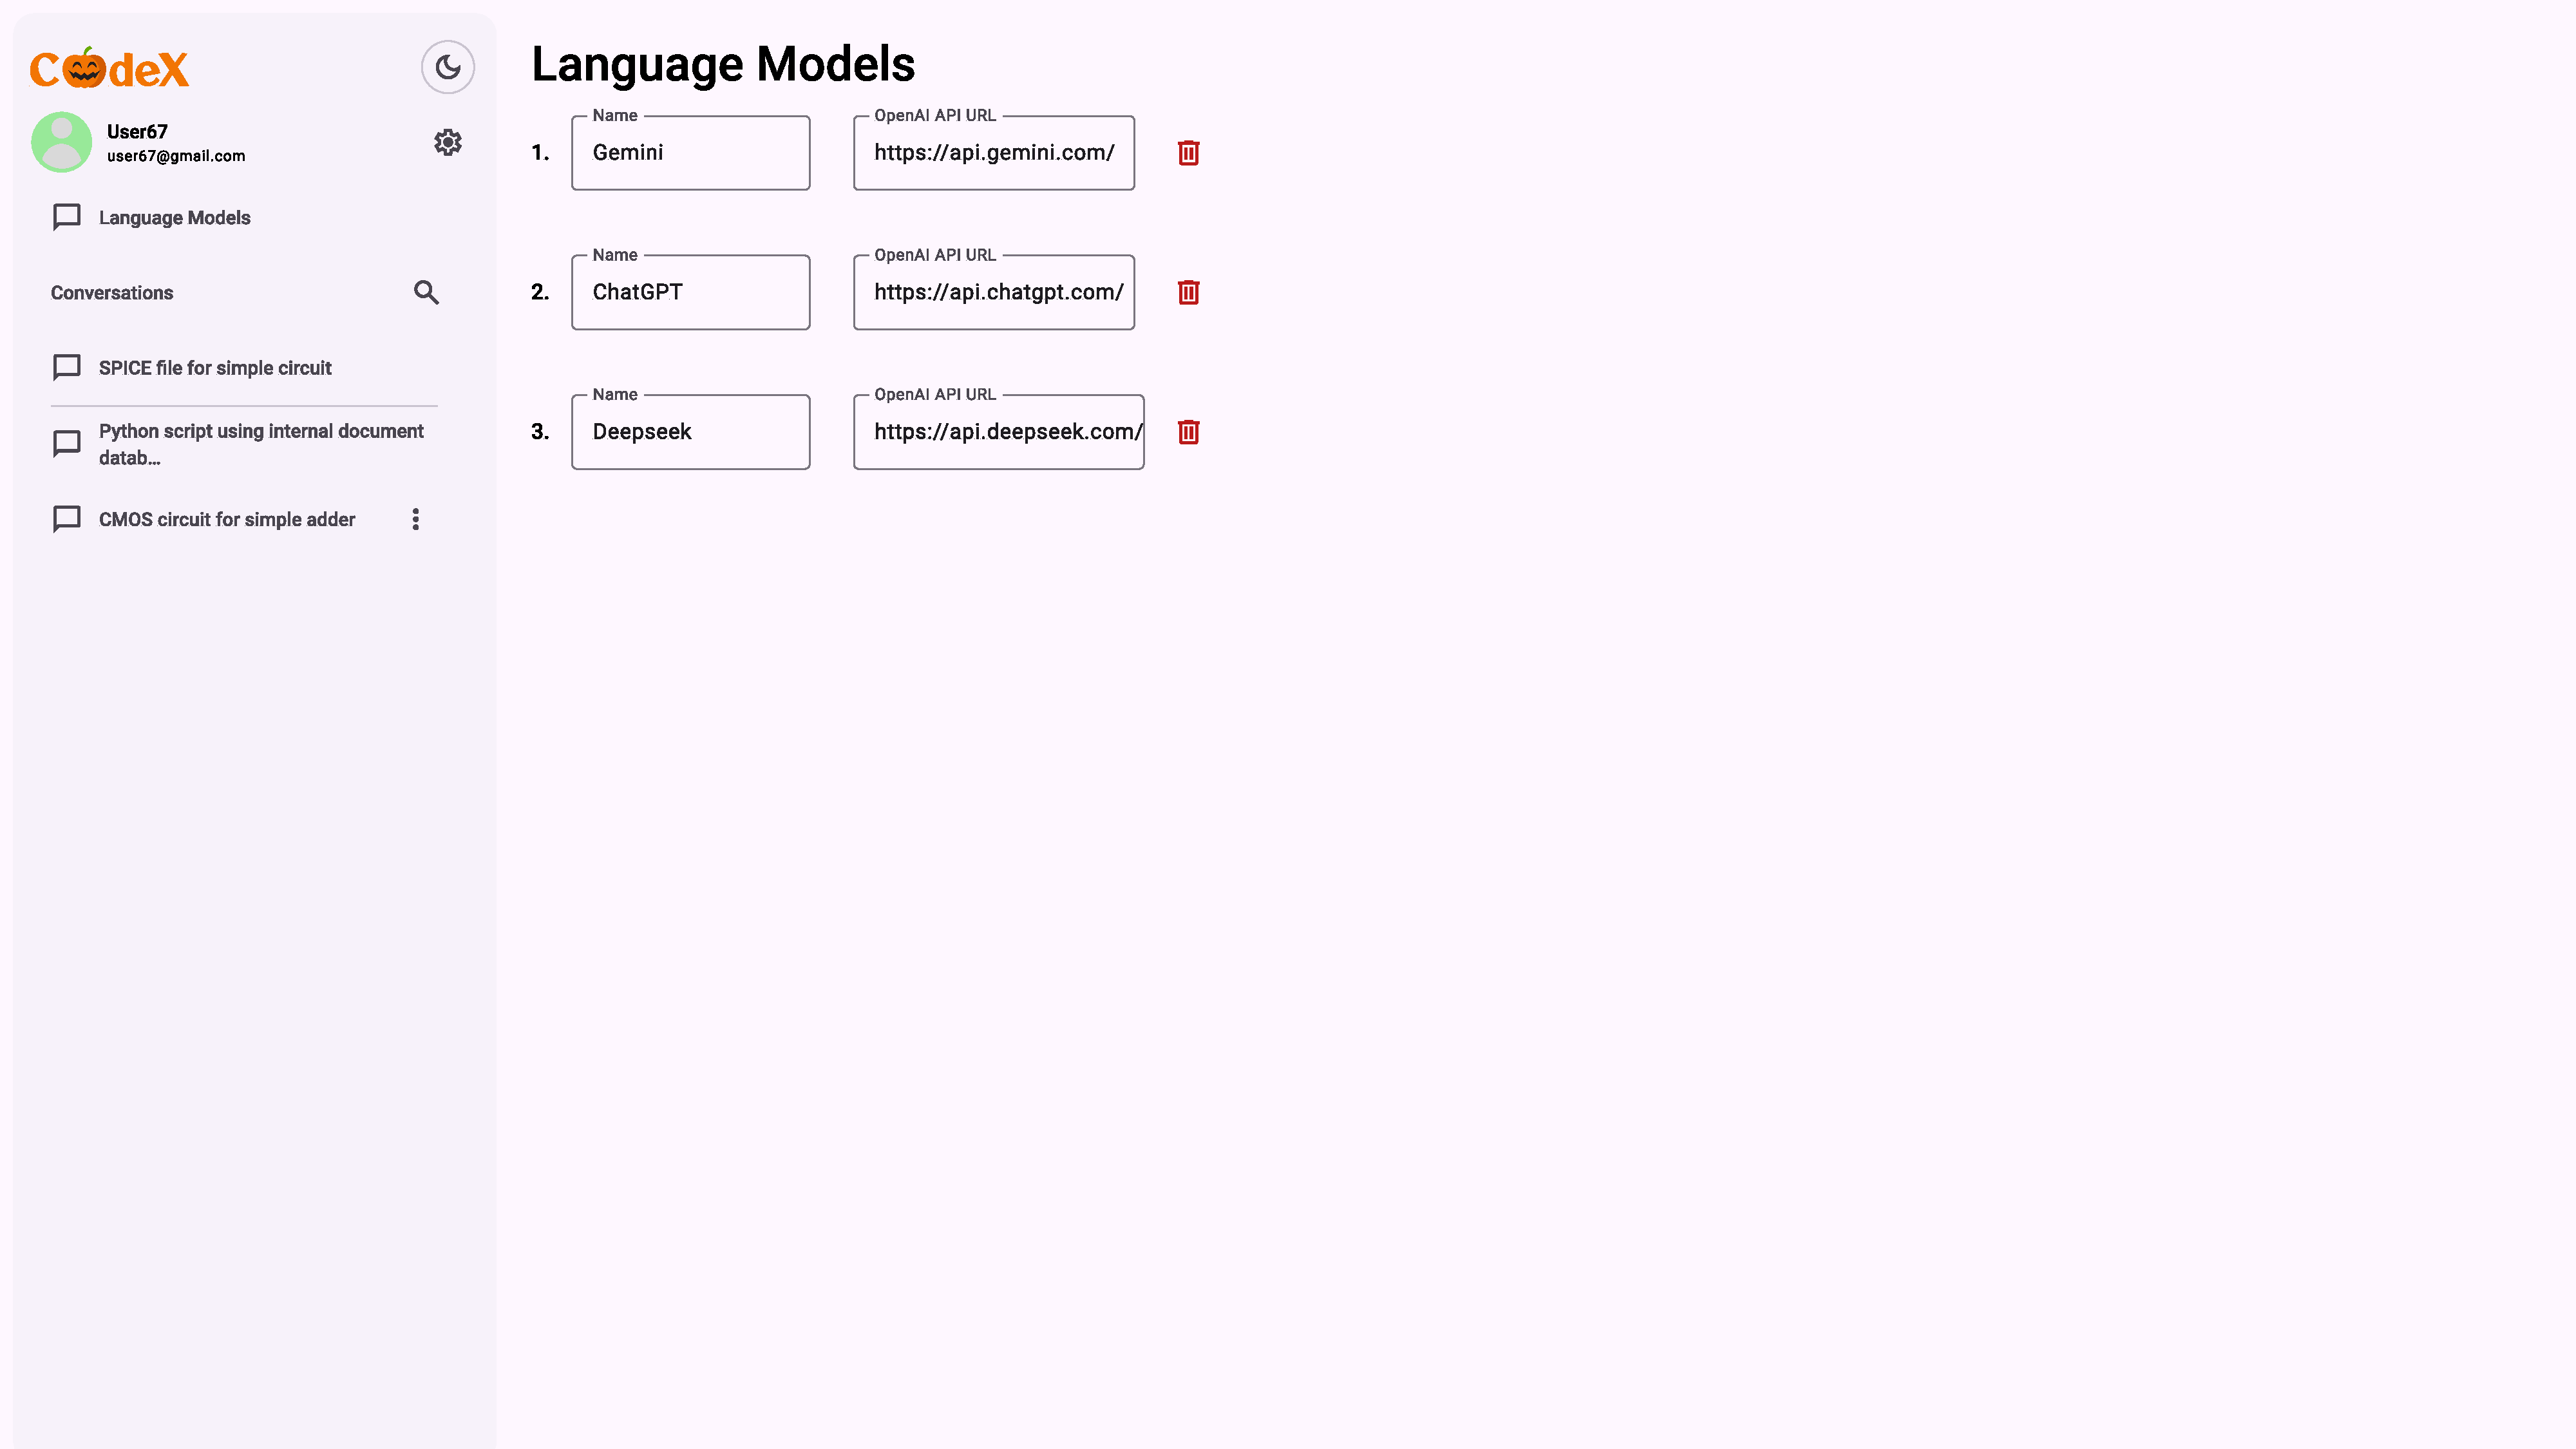
\includegraphics[width=\linewidth]{figures/ui/desktop/Settings_Screen}
    \caption{\hyperref[abr:GUI]{GUI}: Admin panel}
    \label{fig:ui-d-settings}
\end{figure}
\begin{figure}
    \centering
    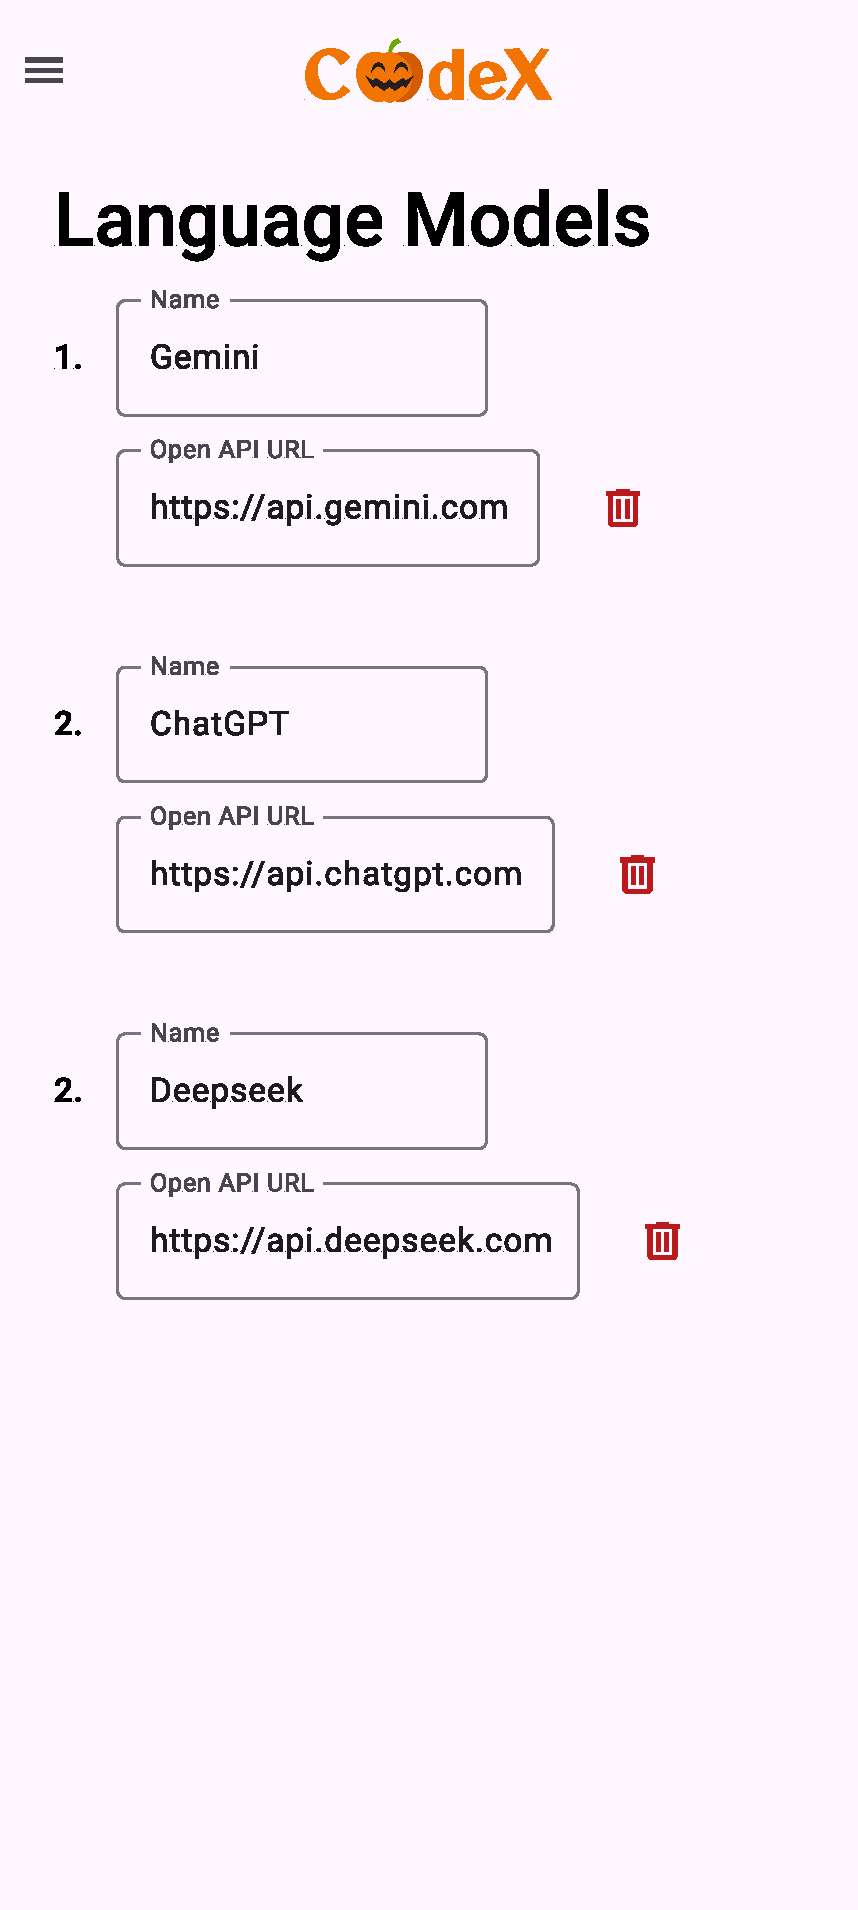
\includegraphics[width=5cm]{figures/ui/mobile/Settings_Screen}
    \caption{\hyperref[abr:GUI]{GUI}: Admin panel (mobile)}
    \label{fig:ui-m-settings}
\end{figure}

\subsection{Log-in}
The log-in screen (\ref{fig:ui-d-login}/\ref{fig:ui-m-login}) allows an unauthenticated user to login by entering the credentials to an account.
Users can also opt to reset their password, go to the signup screen or continue with an \textit{\hyperref[def:oauth]{OAuth} provider}.
\begin{figure}
    \centering
    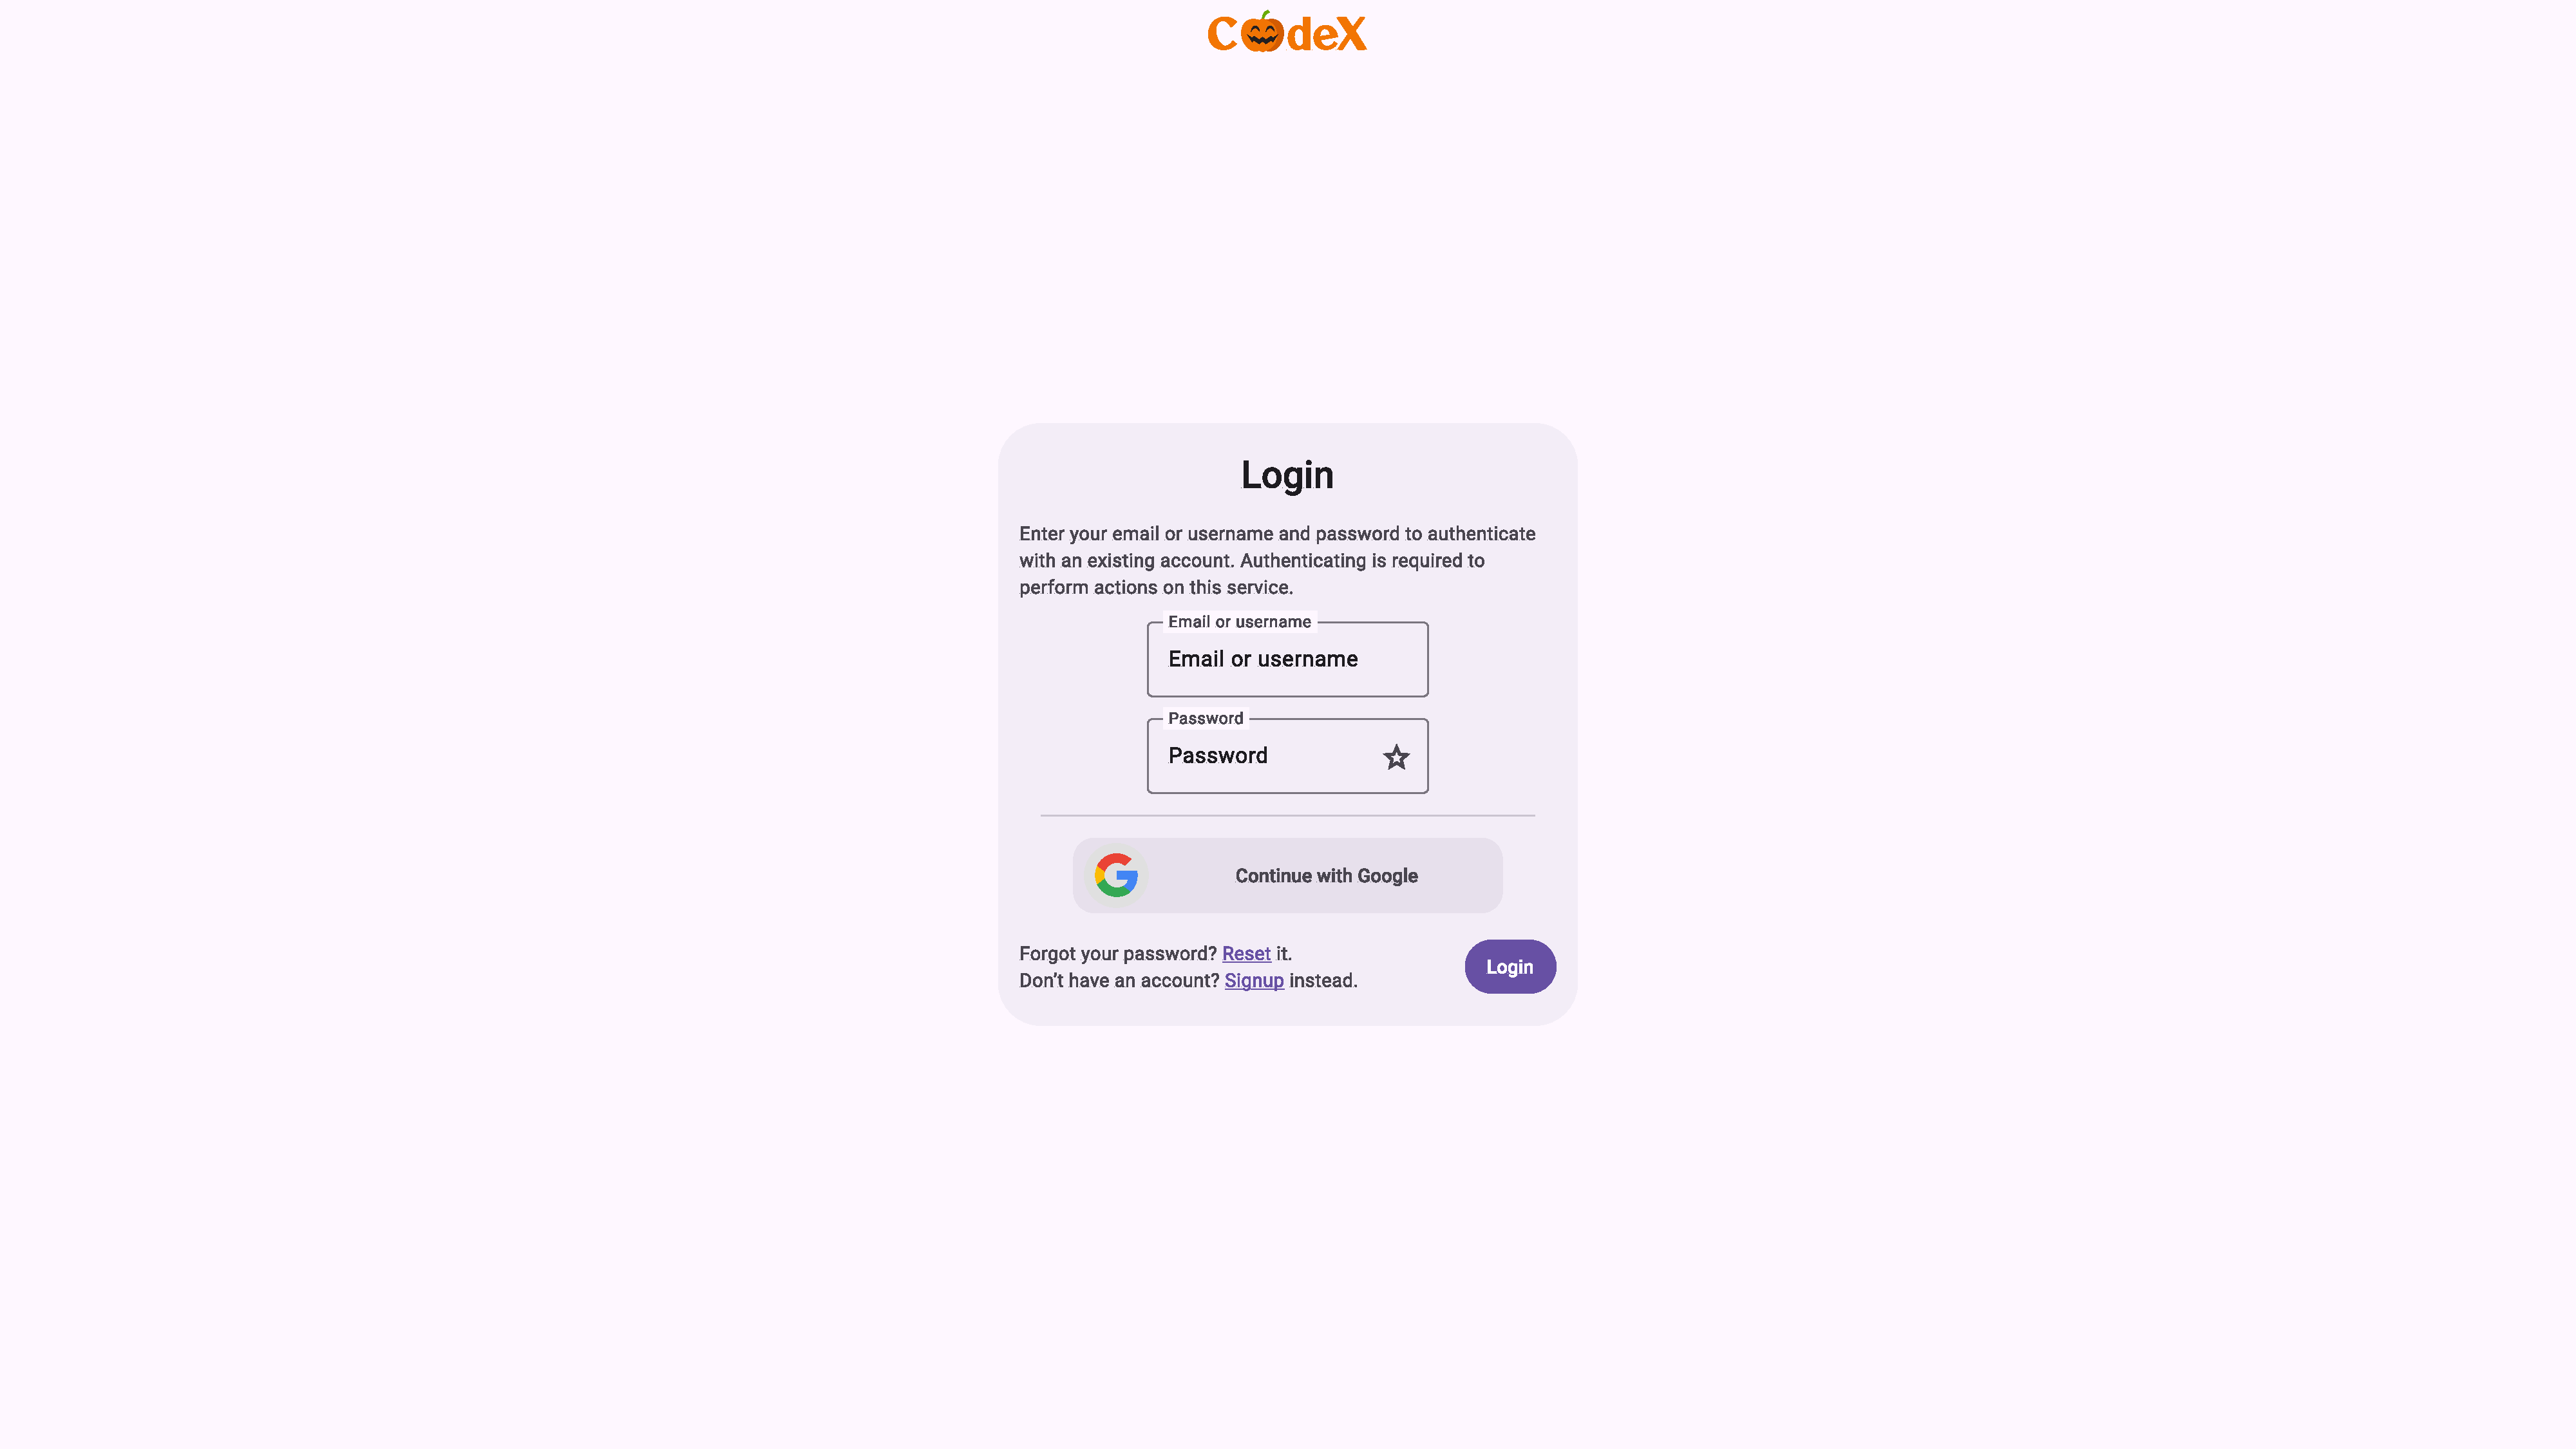
\includegraphics[width=\linewidth]{figures/ui/desktop/Login_Screen}
    \caption{\hyperref[abr:GUI]{GUI}: Log-in screen}
    \label{fig:ui-d-login}
\end{figure}
\begin{figure}
    \centering
    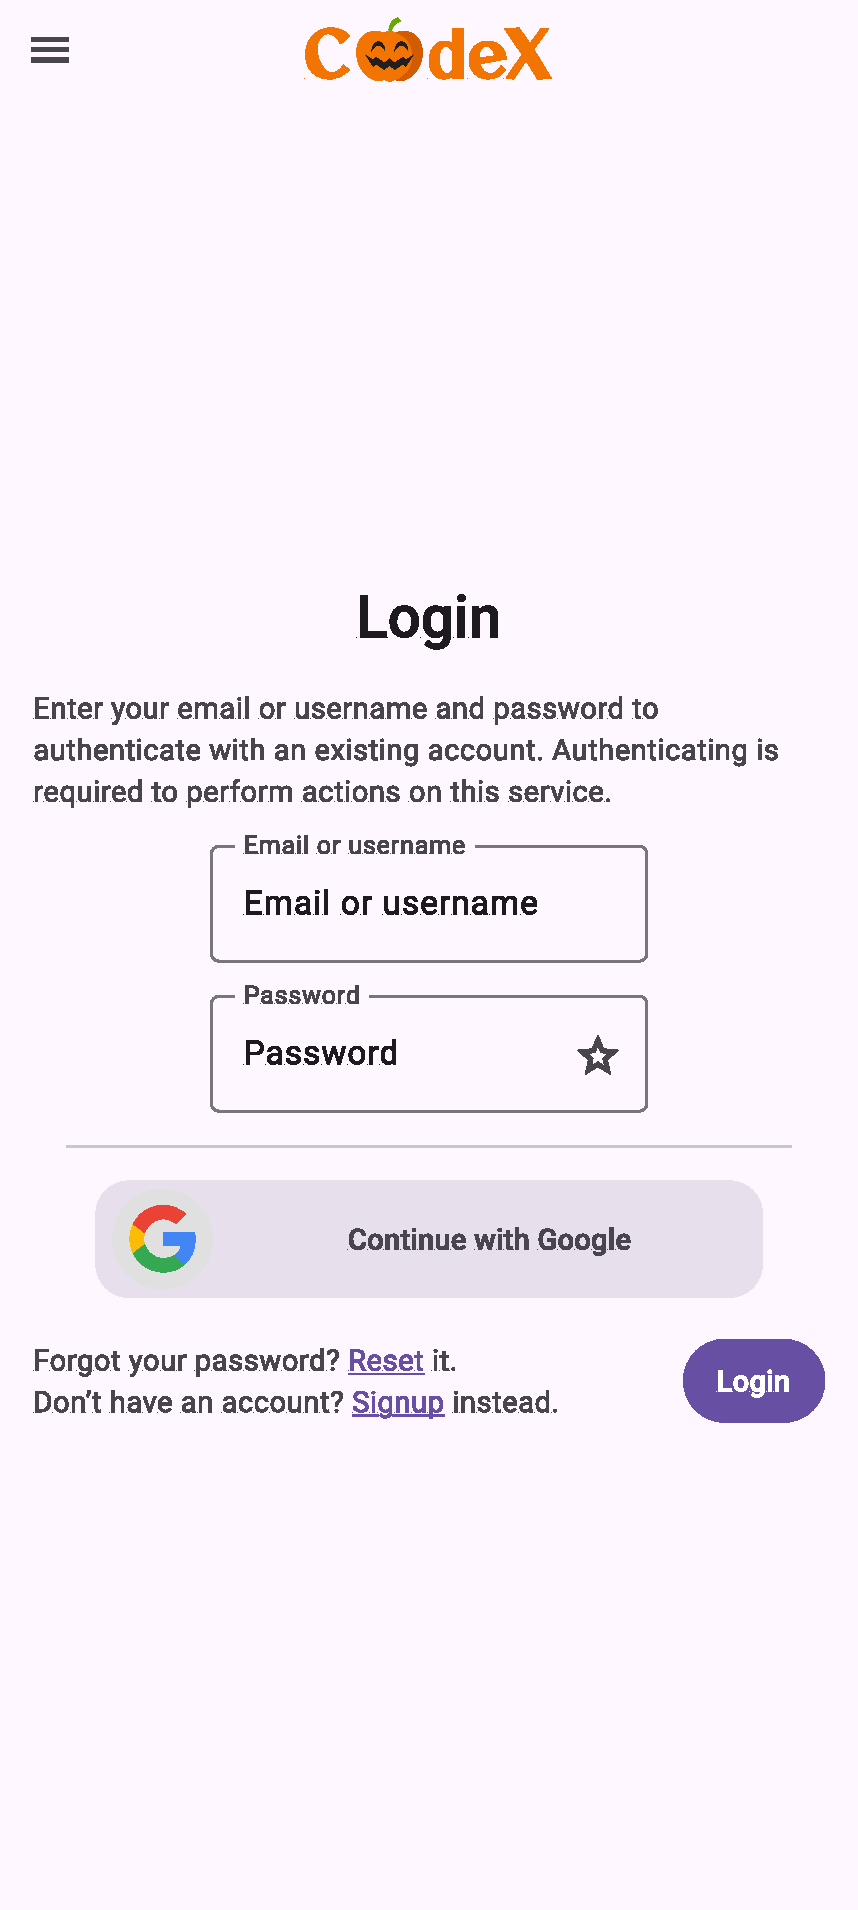
\includegraphics[width=5cm]{figures/ui/mobile/Login_Screen}
    \caption{\hyperref[abr:GUI]{GUI}: Log-in screen (mobile)}
    \label{fig:ui-m-login}
\end{figure}

\subsection{Request password reset}
The request password reset allows users that lost access to their account to request a password reset.
Users can enter the email of their account (\ref{fig:ui-d-request-reset-password-initial}/\ref{fig:ui-m-request-reset-password-initial}) and after confirming, an informative message is shown (\ref{fig:ui-d-request-reset-password-requested}/\ref{fig:ui-m-request-reset-password-requested}).
\begin{figure}
    \centering
    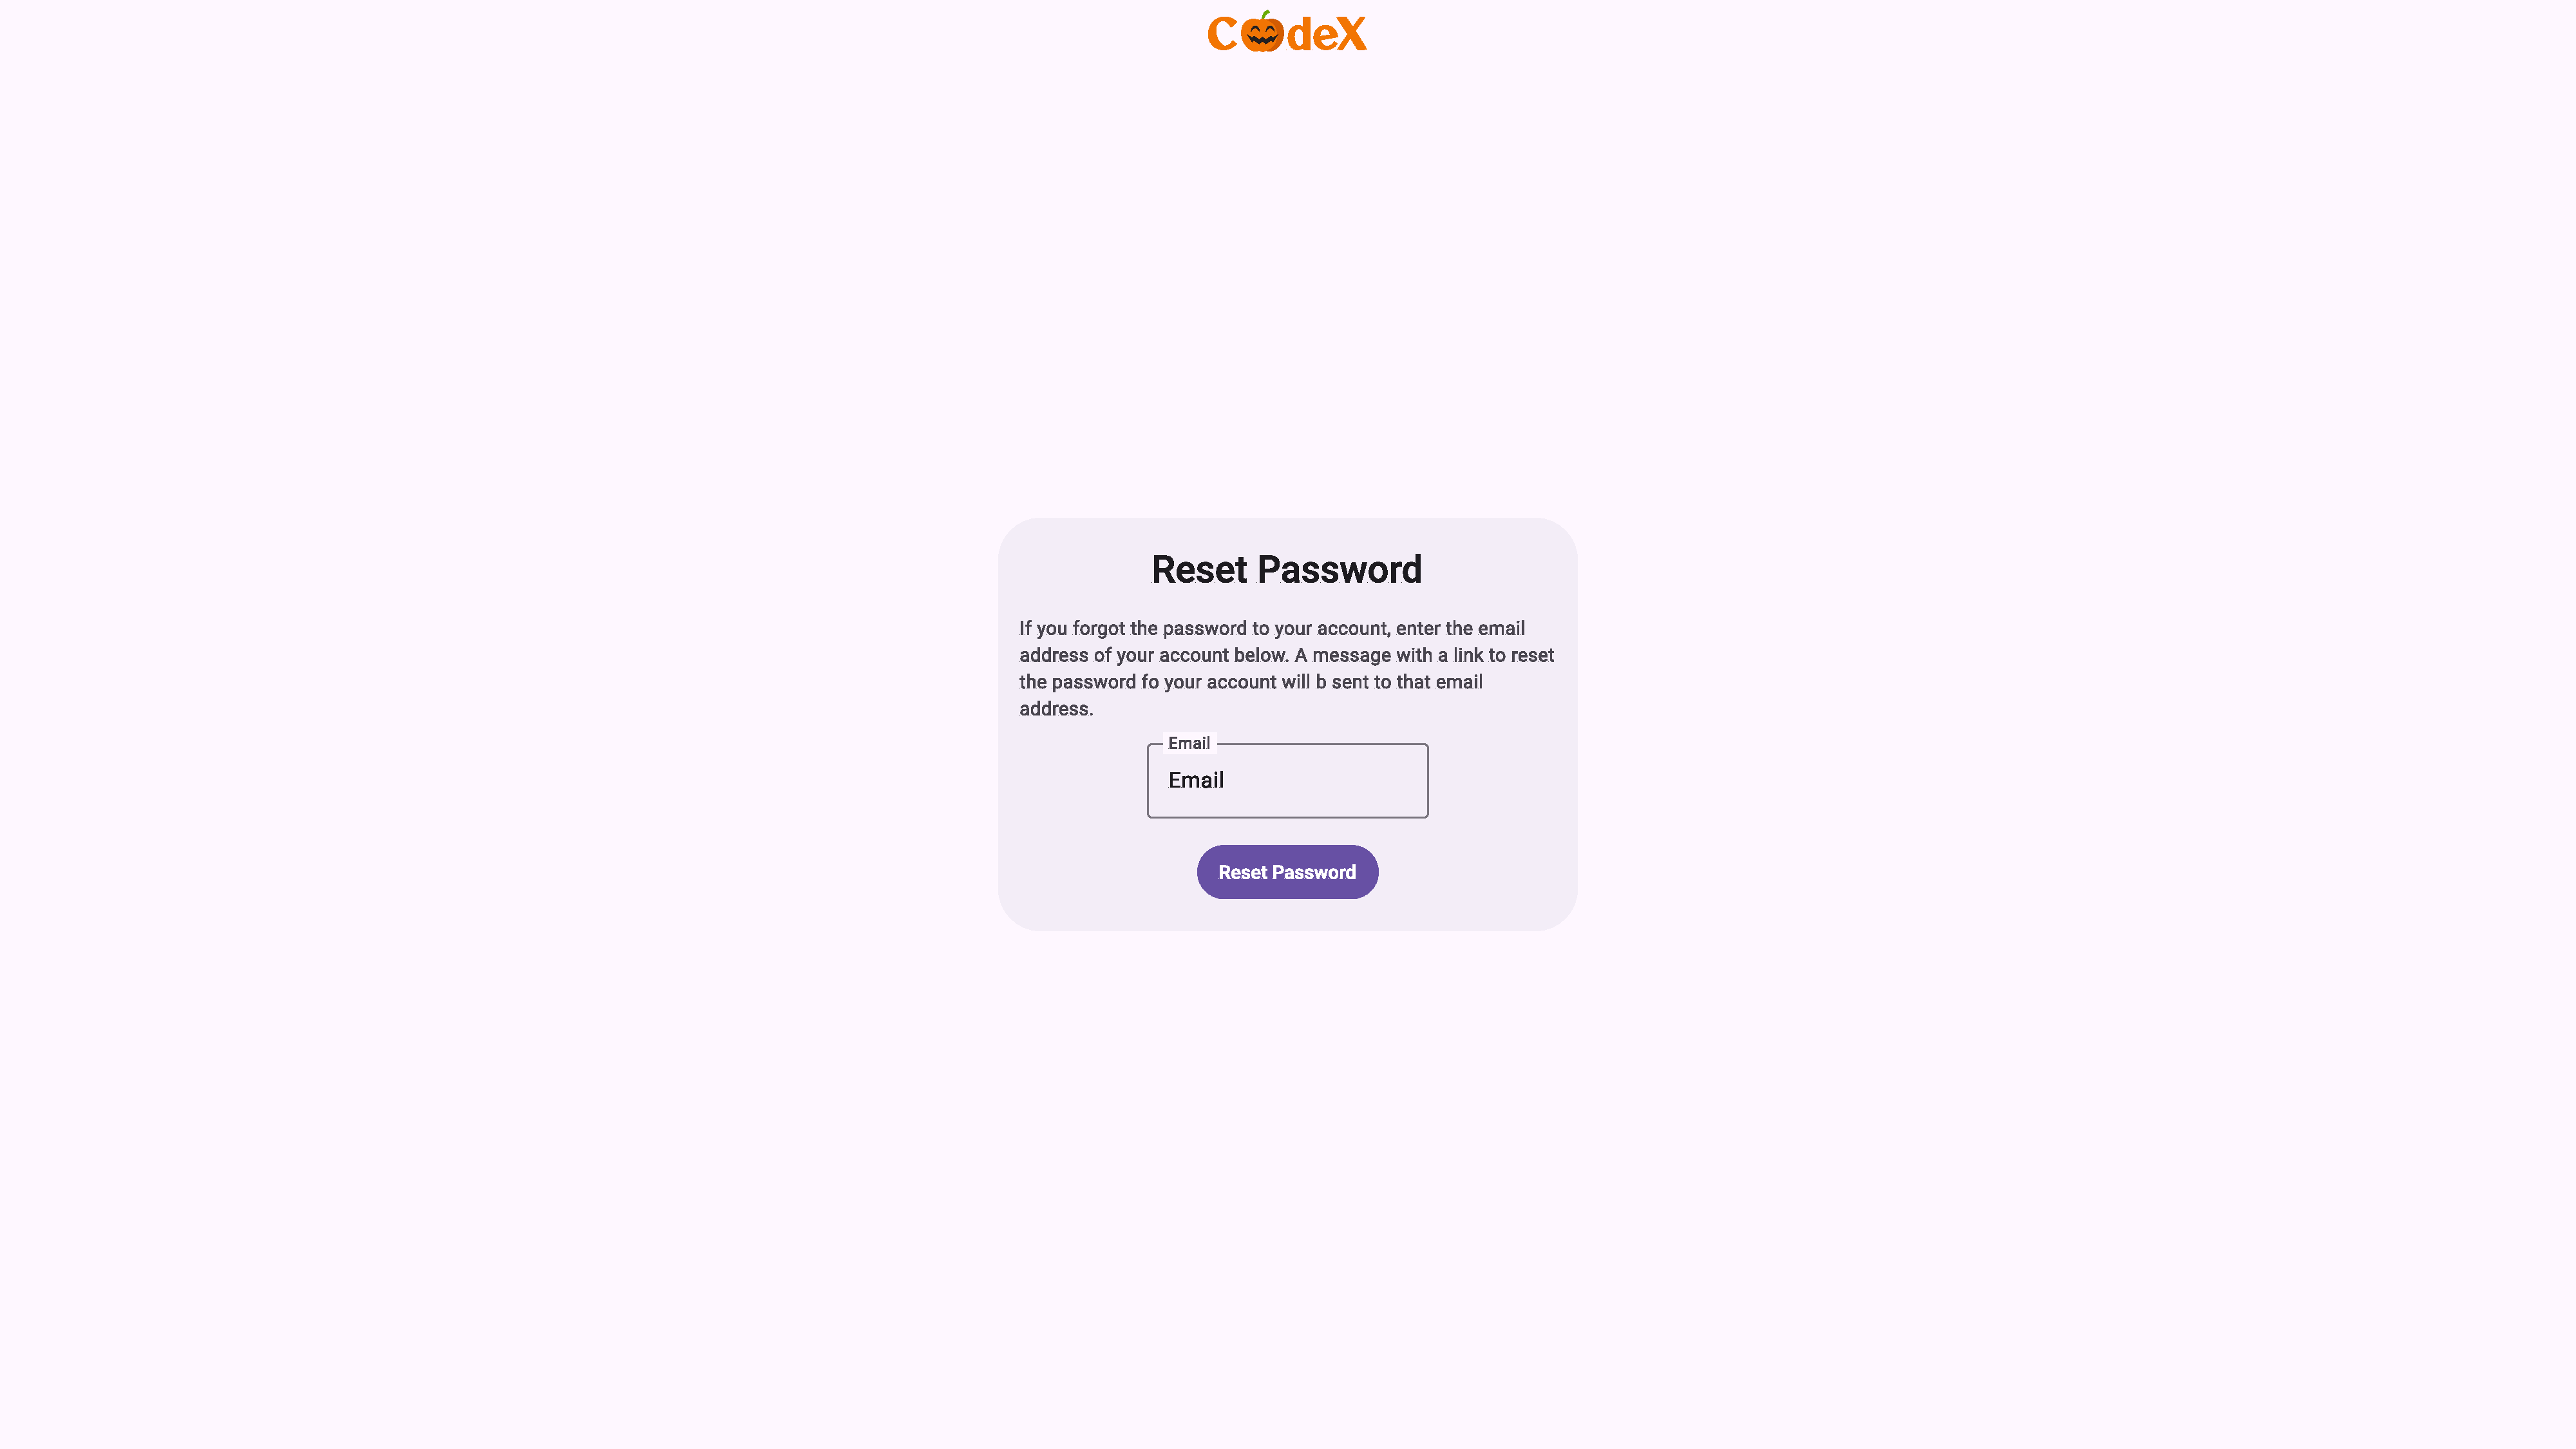
\includegraphics[width=\linewidth]{figures/ui/desktop/Request_Reset_Password_Screen initial}
    \caption{\hyperref[abr:GUI]{GUI}: Request password screen before requesting}
    \label{fig:ui-d-request-reset-password-initial}
\end{figure}
\begin{figure}
    \centering
    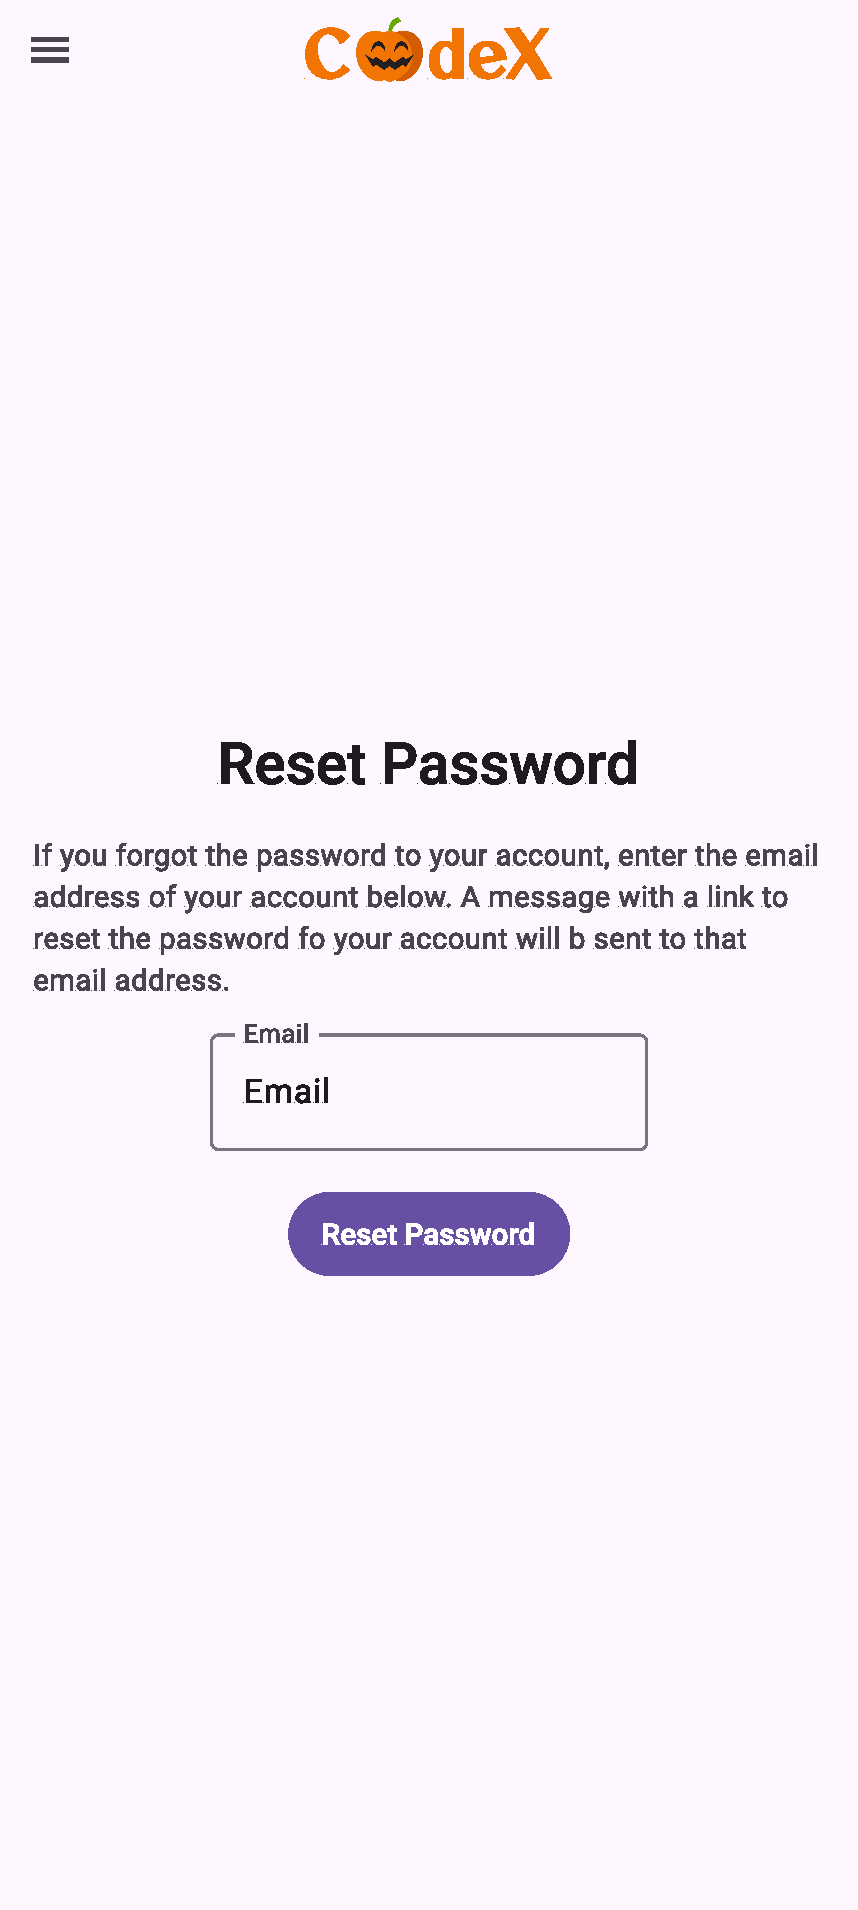
\includegraphics[width=5cm]{figures/ui/mobile/Request_Reset_Password_Screen initial}
    \caption{\hyperref[abr:GUI]{GUI}: Request password screen before requesting (mobile)}
    \label{fig:ui-m-request-reset-password-initial}
\end{figure}

\begin{figure}
    \centering
    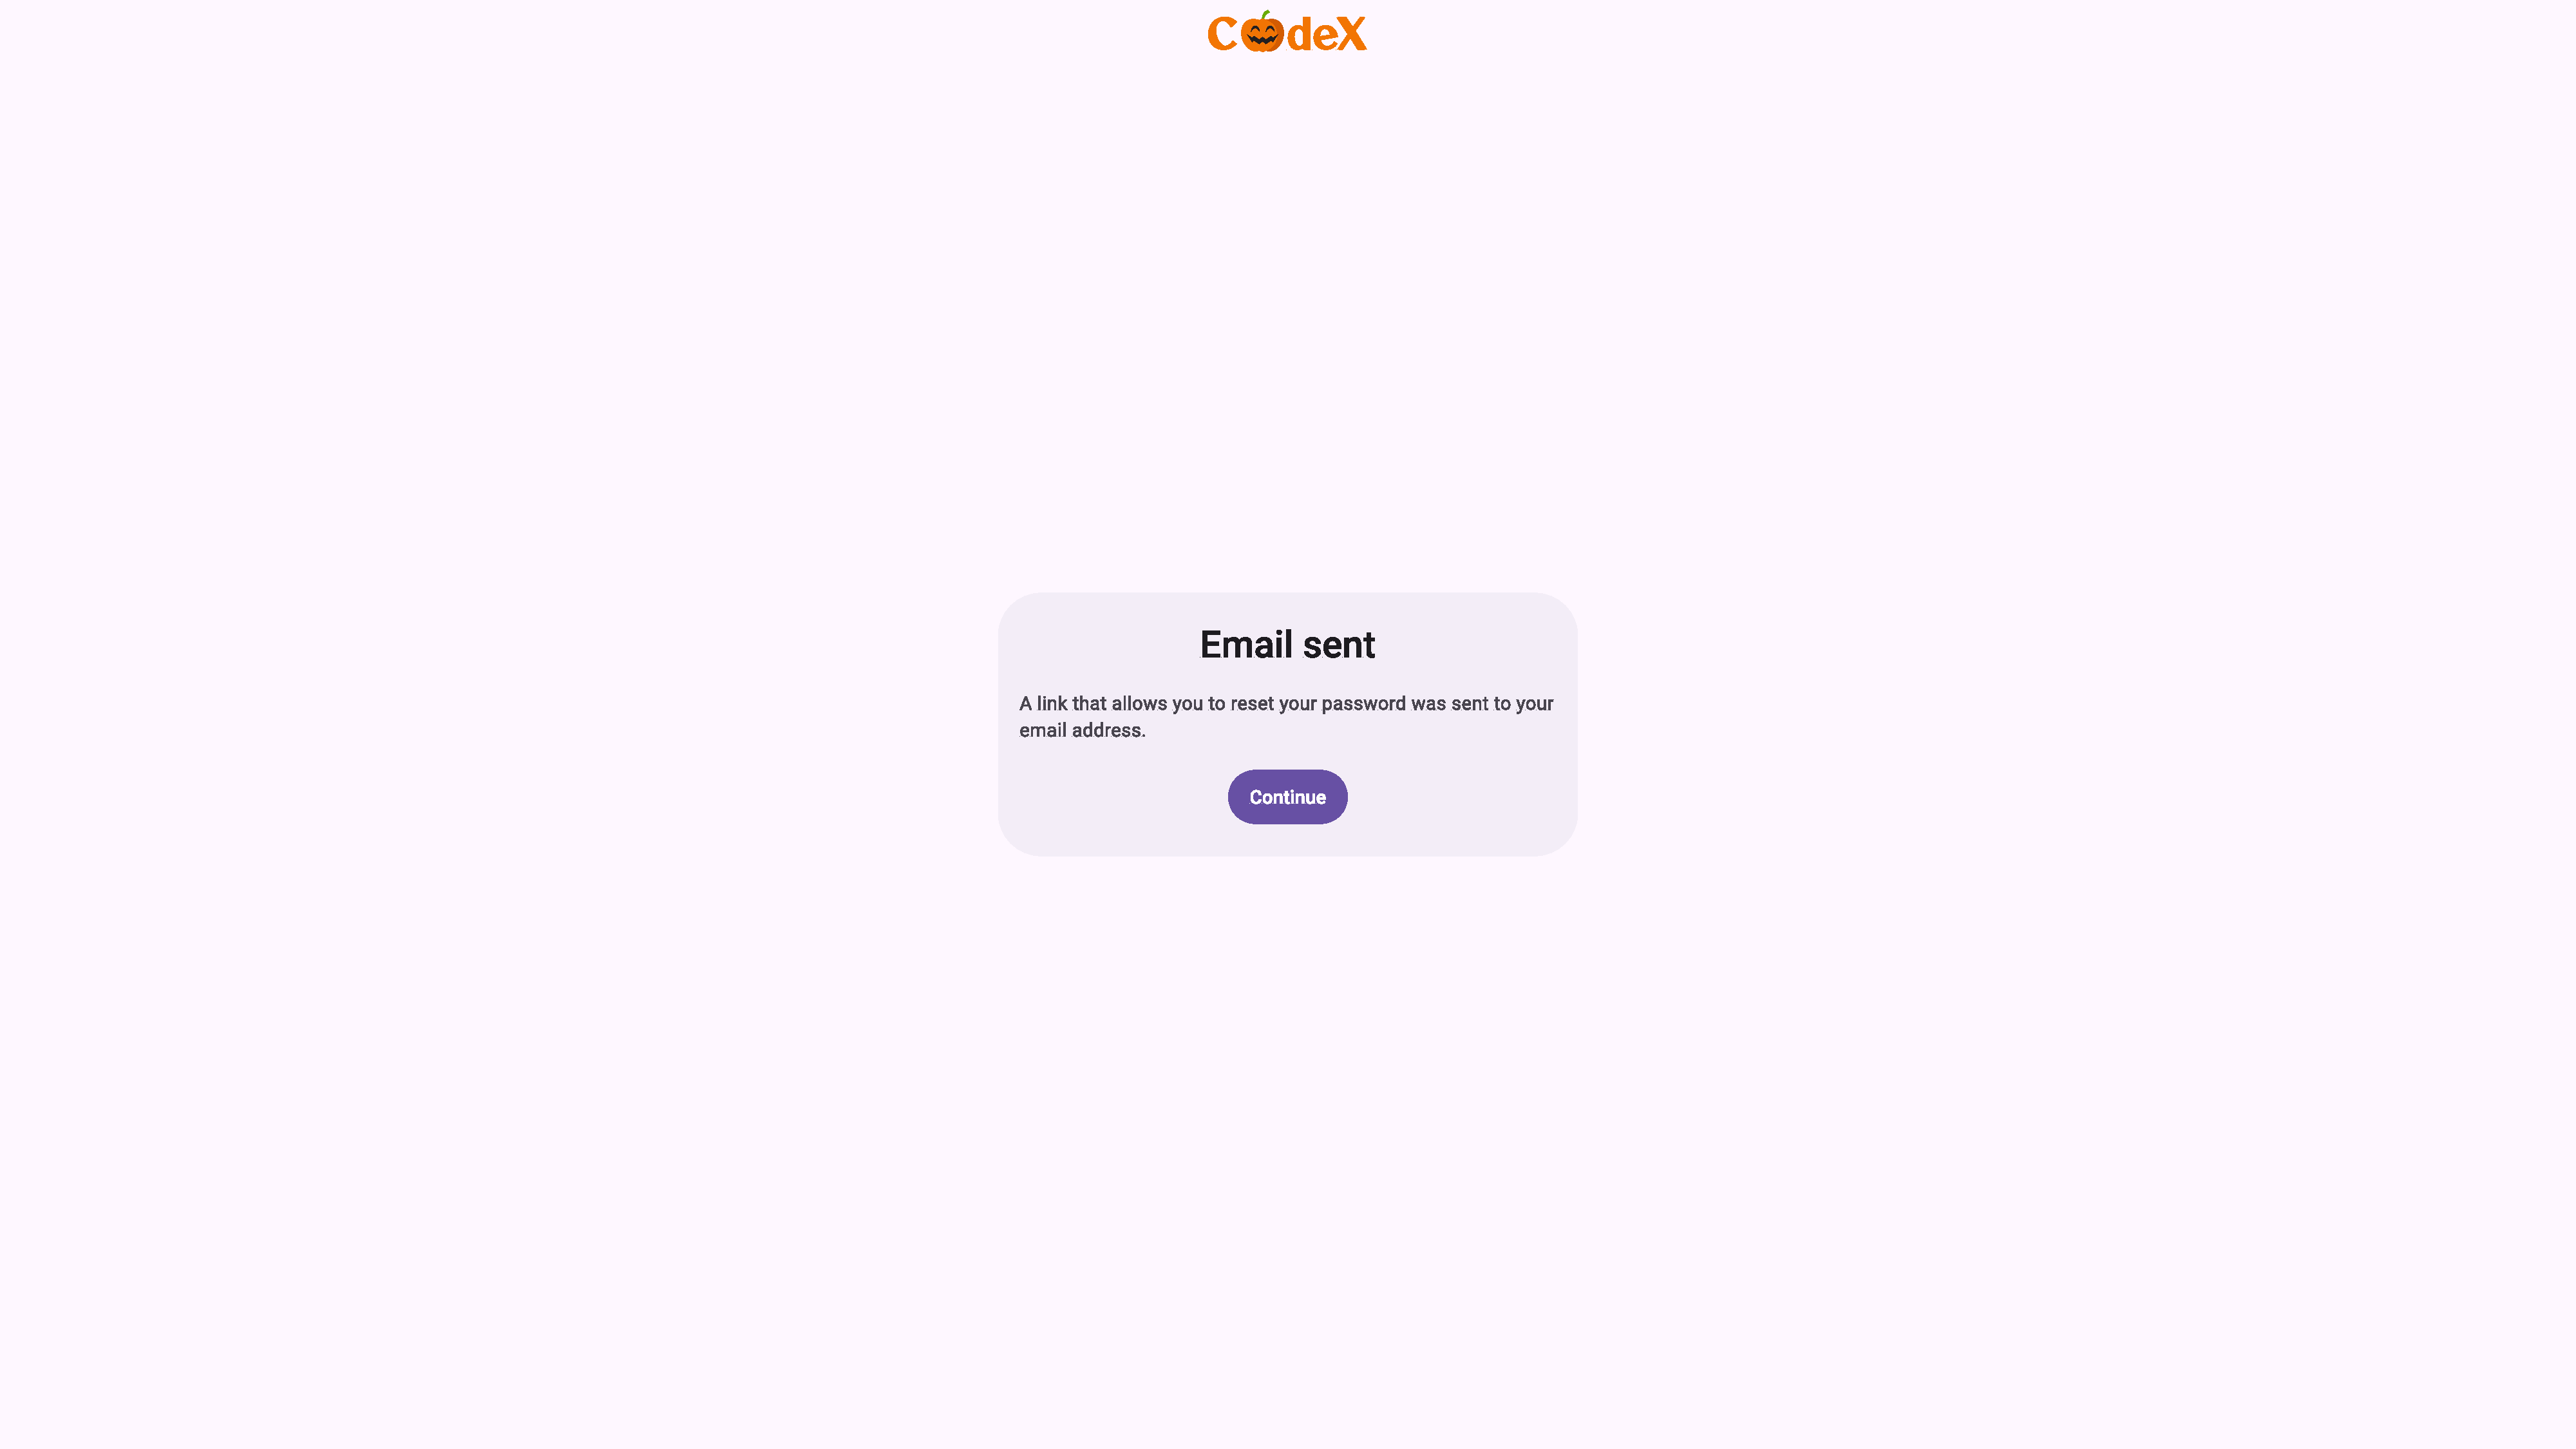
\includegraphics[width=\linewidth]{figures/ui/desktop/Request_Reset_Password_Screen requested}
    \caption{\hyperref[abr:GUI]{GUI}: Request password screen after requesting}
    \label{fig:ui-d-request-reset-password-requested}
\end{figure}
\begin{figure}
    \centering
    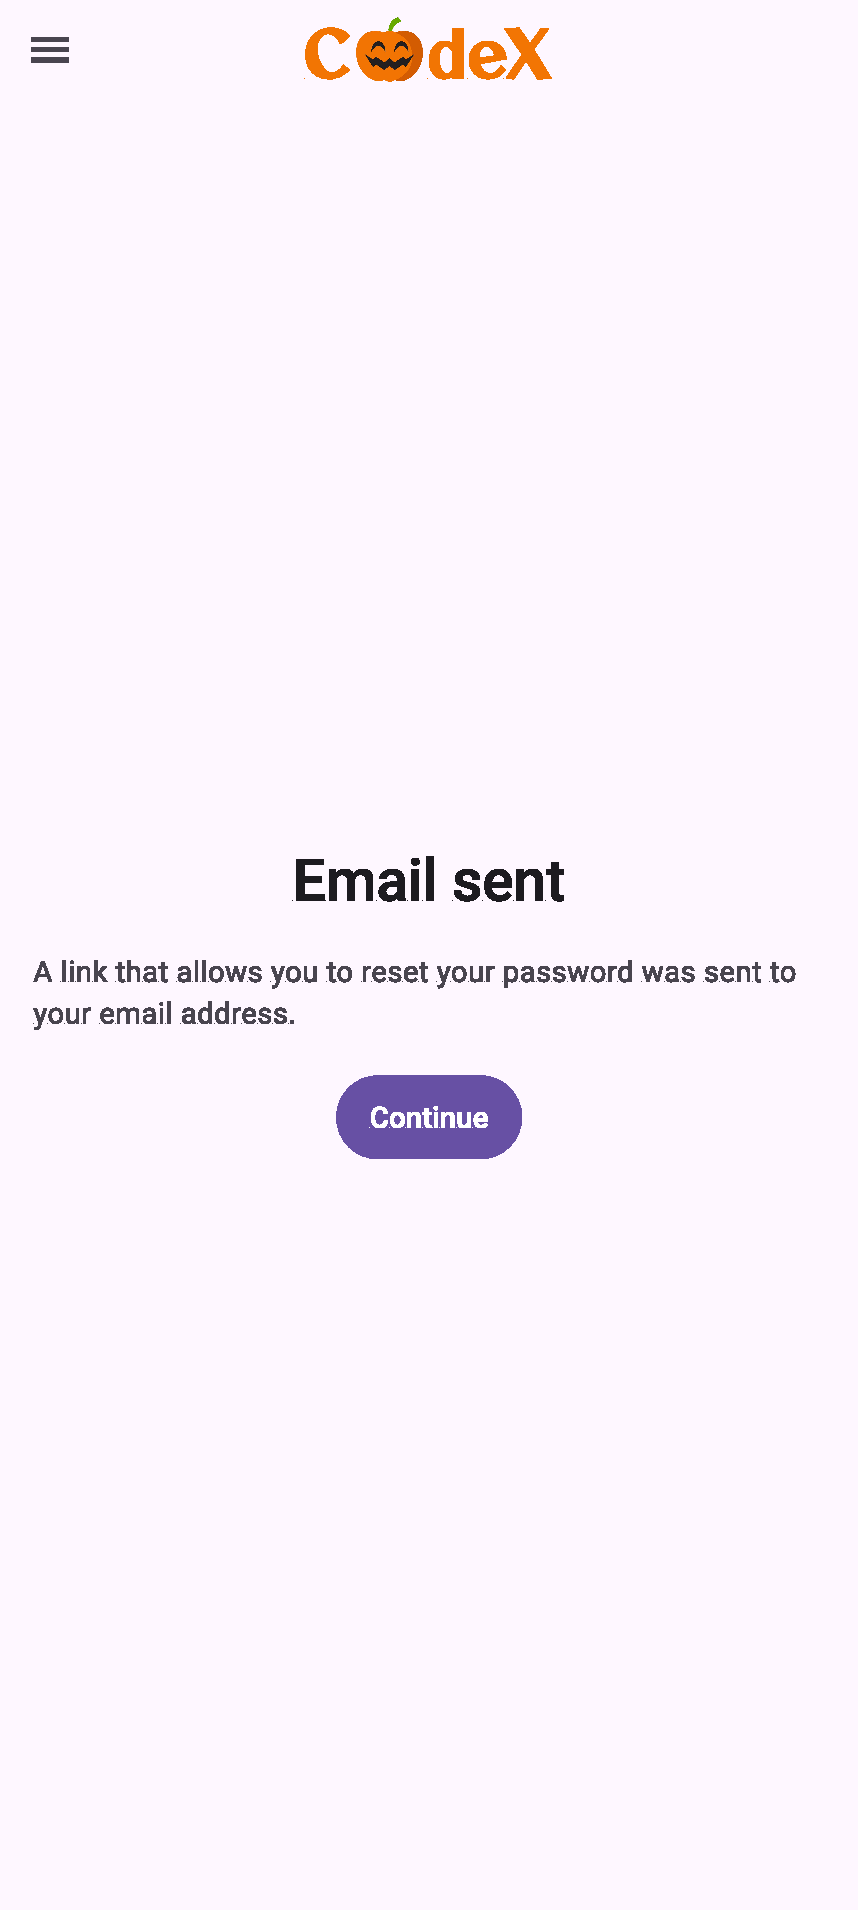
\includegraphics[width=5cm]{figures/ui/mobile/Request_Reset_Password_Screen requested}
    \caption{\hyperref[abr:GUI]{GUI}: Request password screen after requesting (mobile)}
    \label{fig:ui-m-request-reset-password-requested}
\end{figure}

\subsection{Password reset}
The password reset screen allows users to set a new password for their account.
This screen is reached by clicking the link that the user received via mail. \newline
Users can enter a new password (\ref{fig:ui-d-reset-password-initial}/\ref{fig:ui-m-reset-password-initial}), after which an informative message is shown (\ref{fig:ui-d-reset-password-reset}/\ref{fig:ui-m-reset-password-reset}).
\begin{figure}
    \centering
    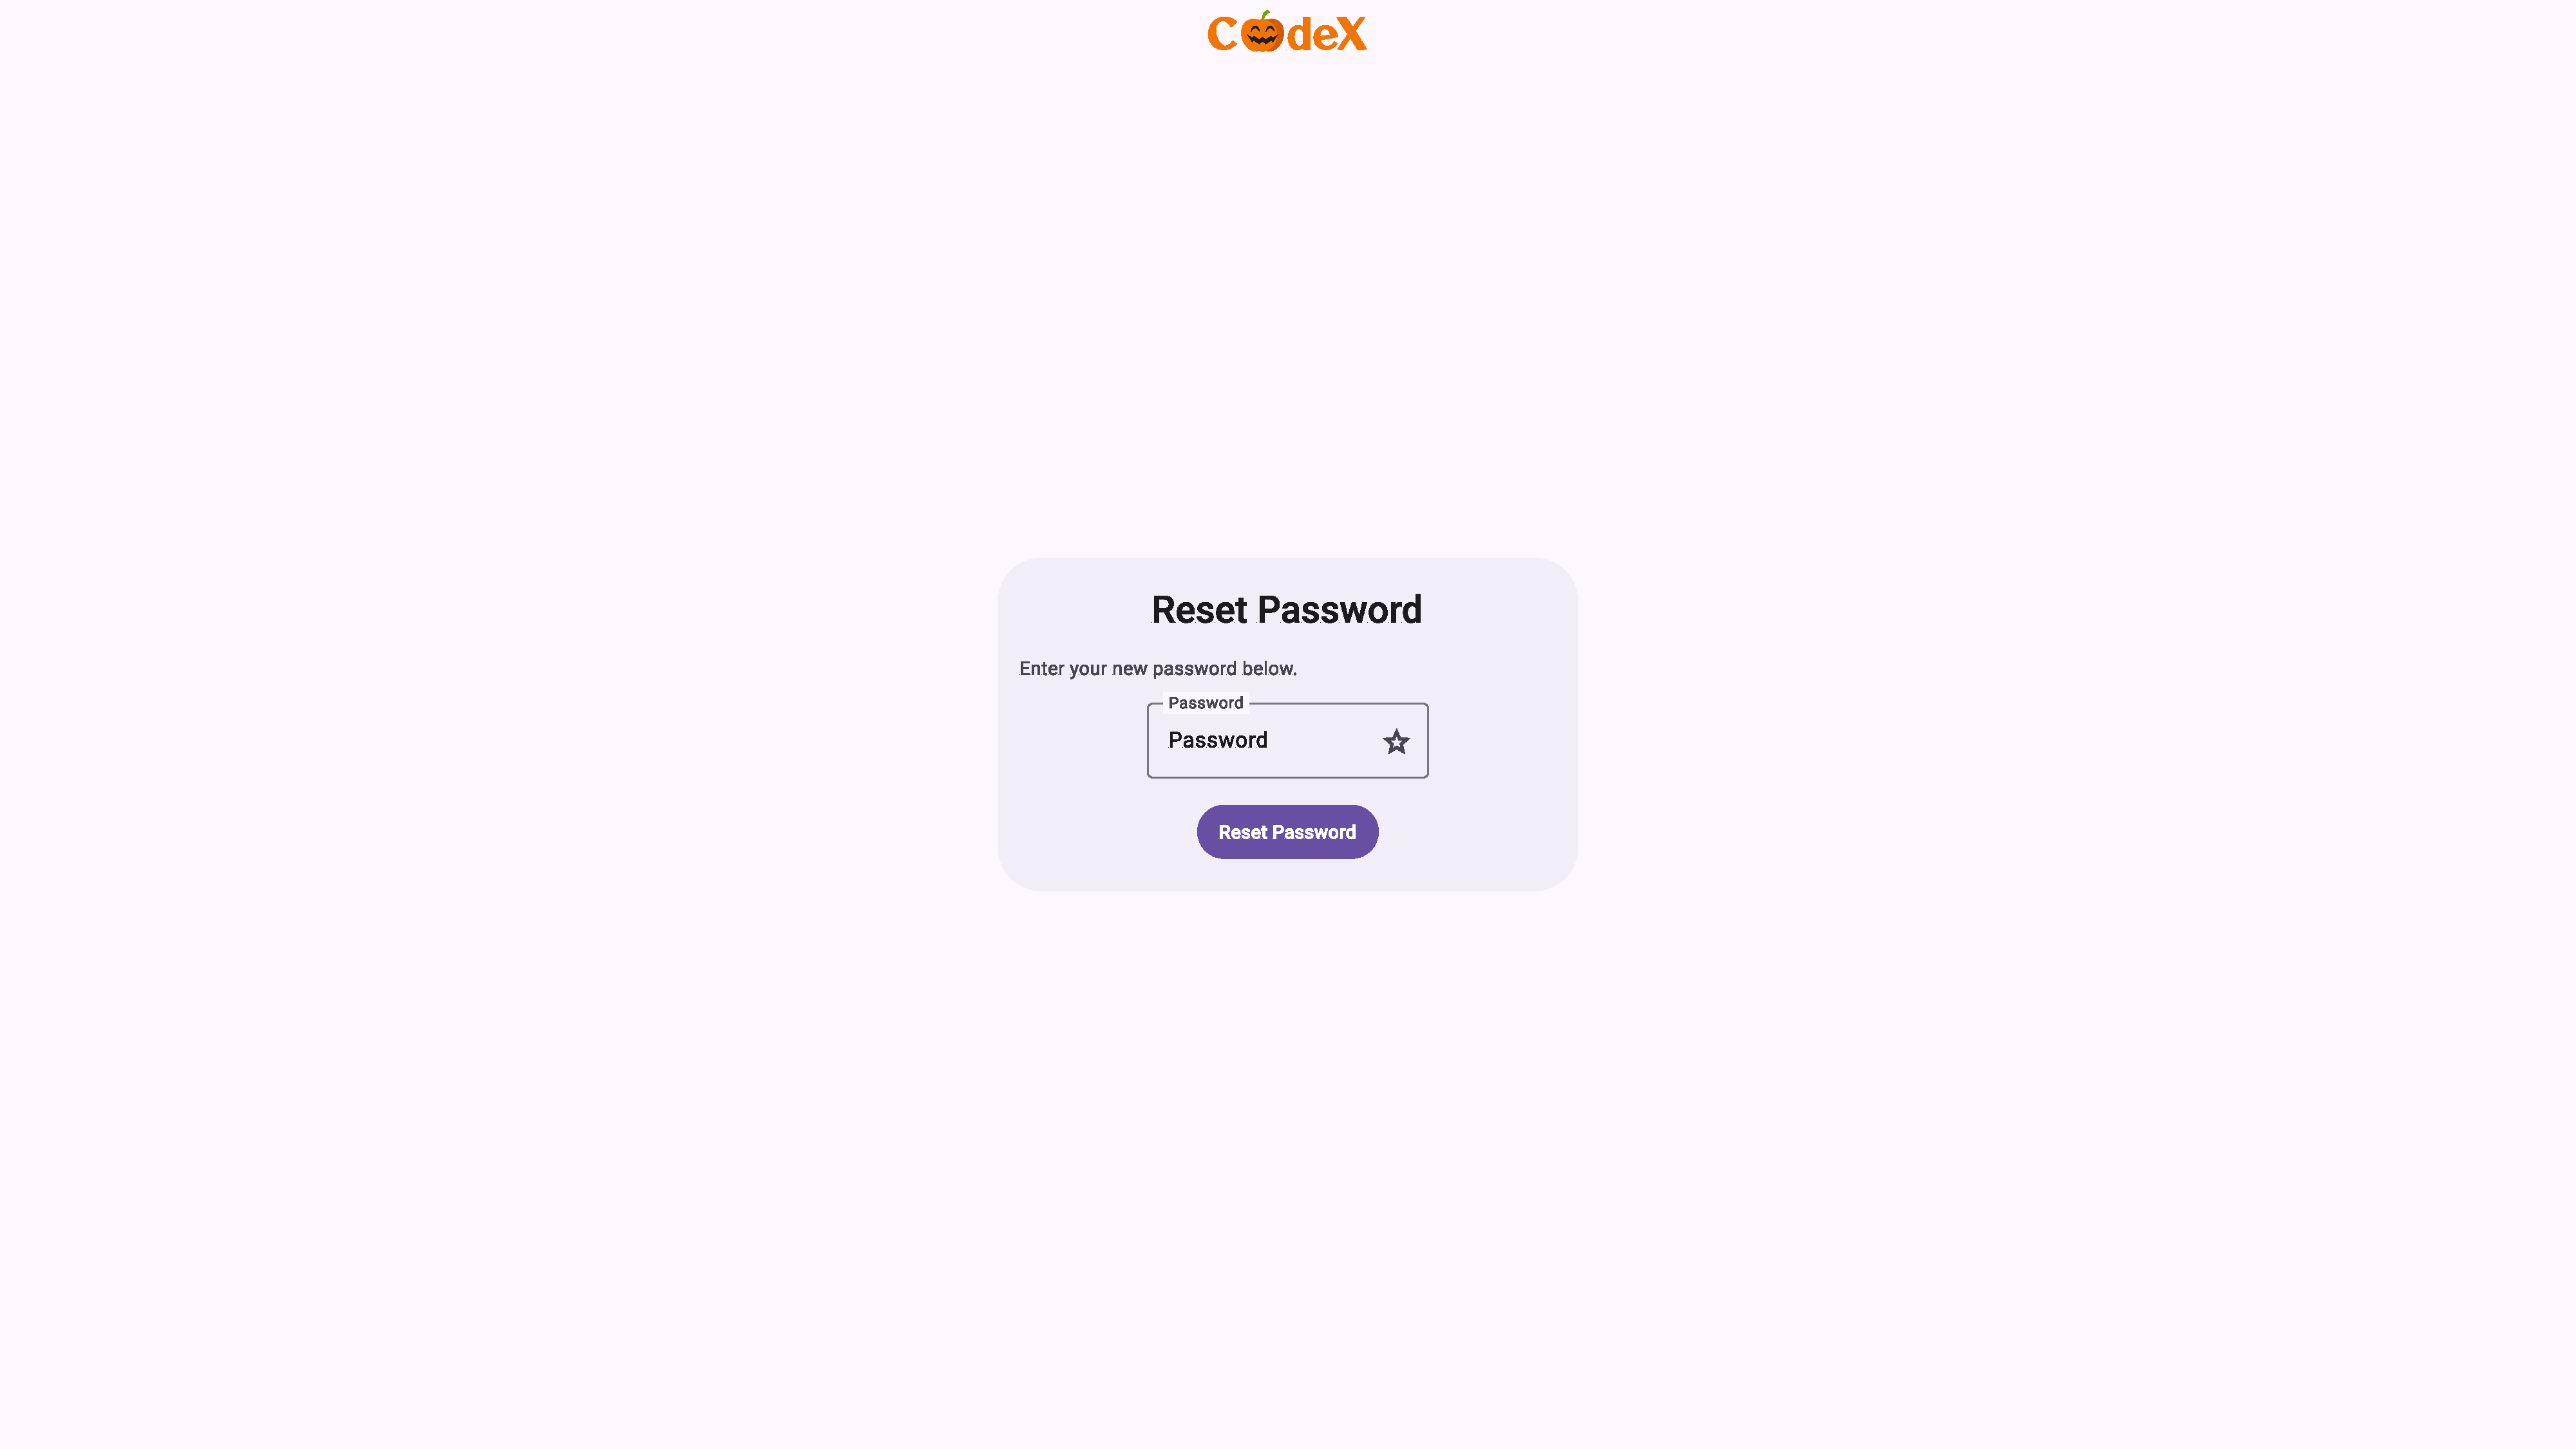
\includegraphics[width=\linewidth]{figures/ui/desktop/Reset_Password_Screen initial}
    \caption{\hyperref[abr:GUI]{GUI}: Reset password screen}
    \label{fig:ui-d-reset-password-initial}
\end{figure}
\begin{figure}
    \centering
    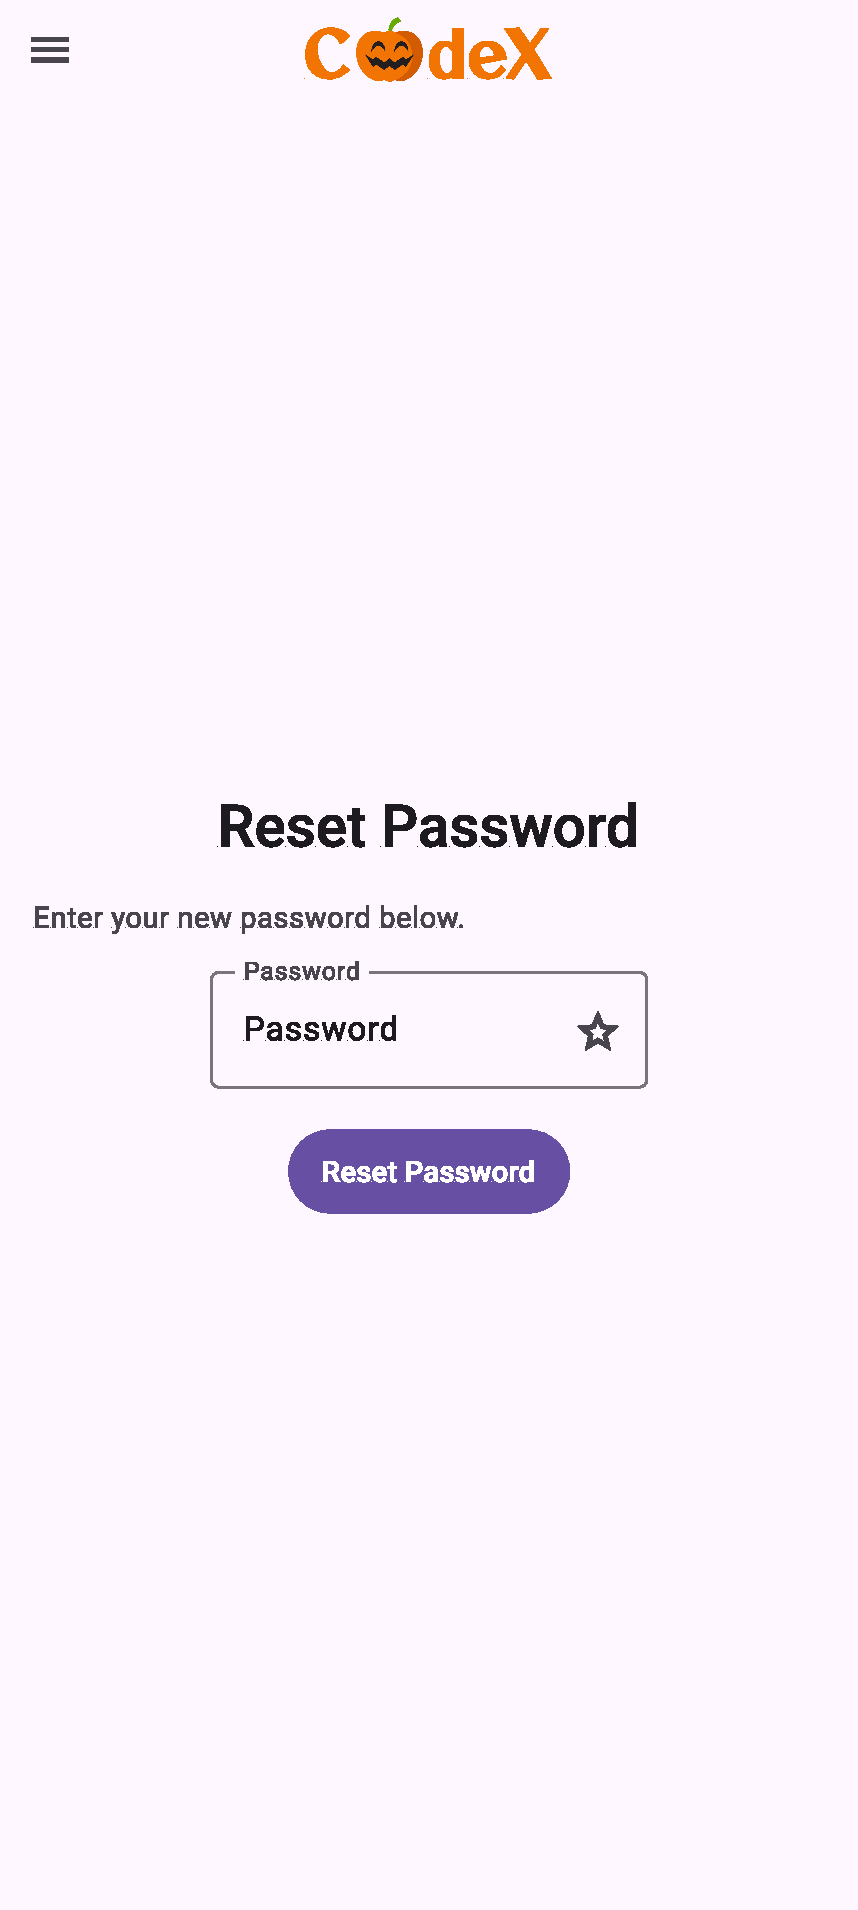
\includegraphics[width=5cm]{figures/ui/mobile/Reset_Password_Screen initial}
    \caption{\hyperref[abr:GUI]{GUI}: Reset password screen (mobile)}
    \label{fig:ui-m-reset-password-initial}
\end{figure}

\begin{figure}
    \centering
    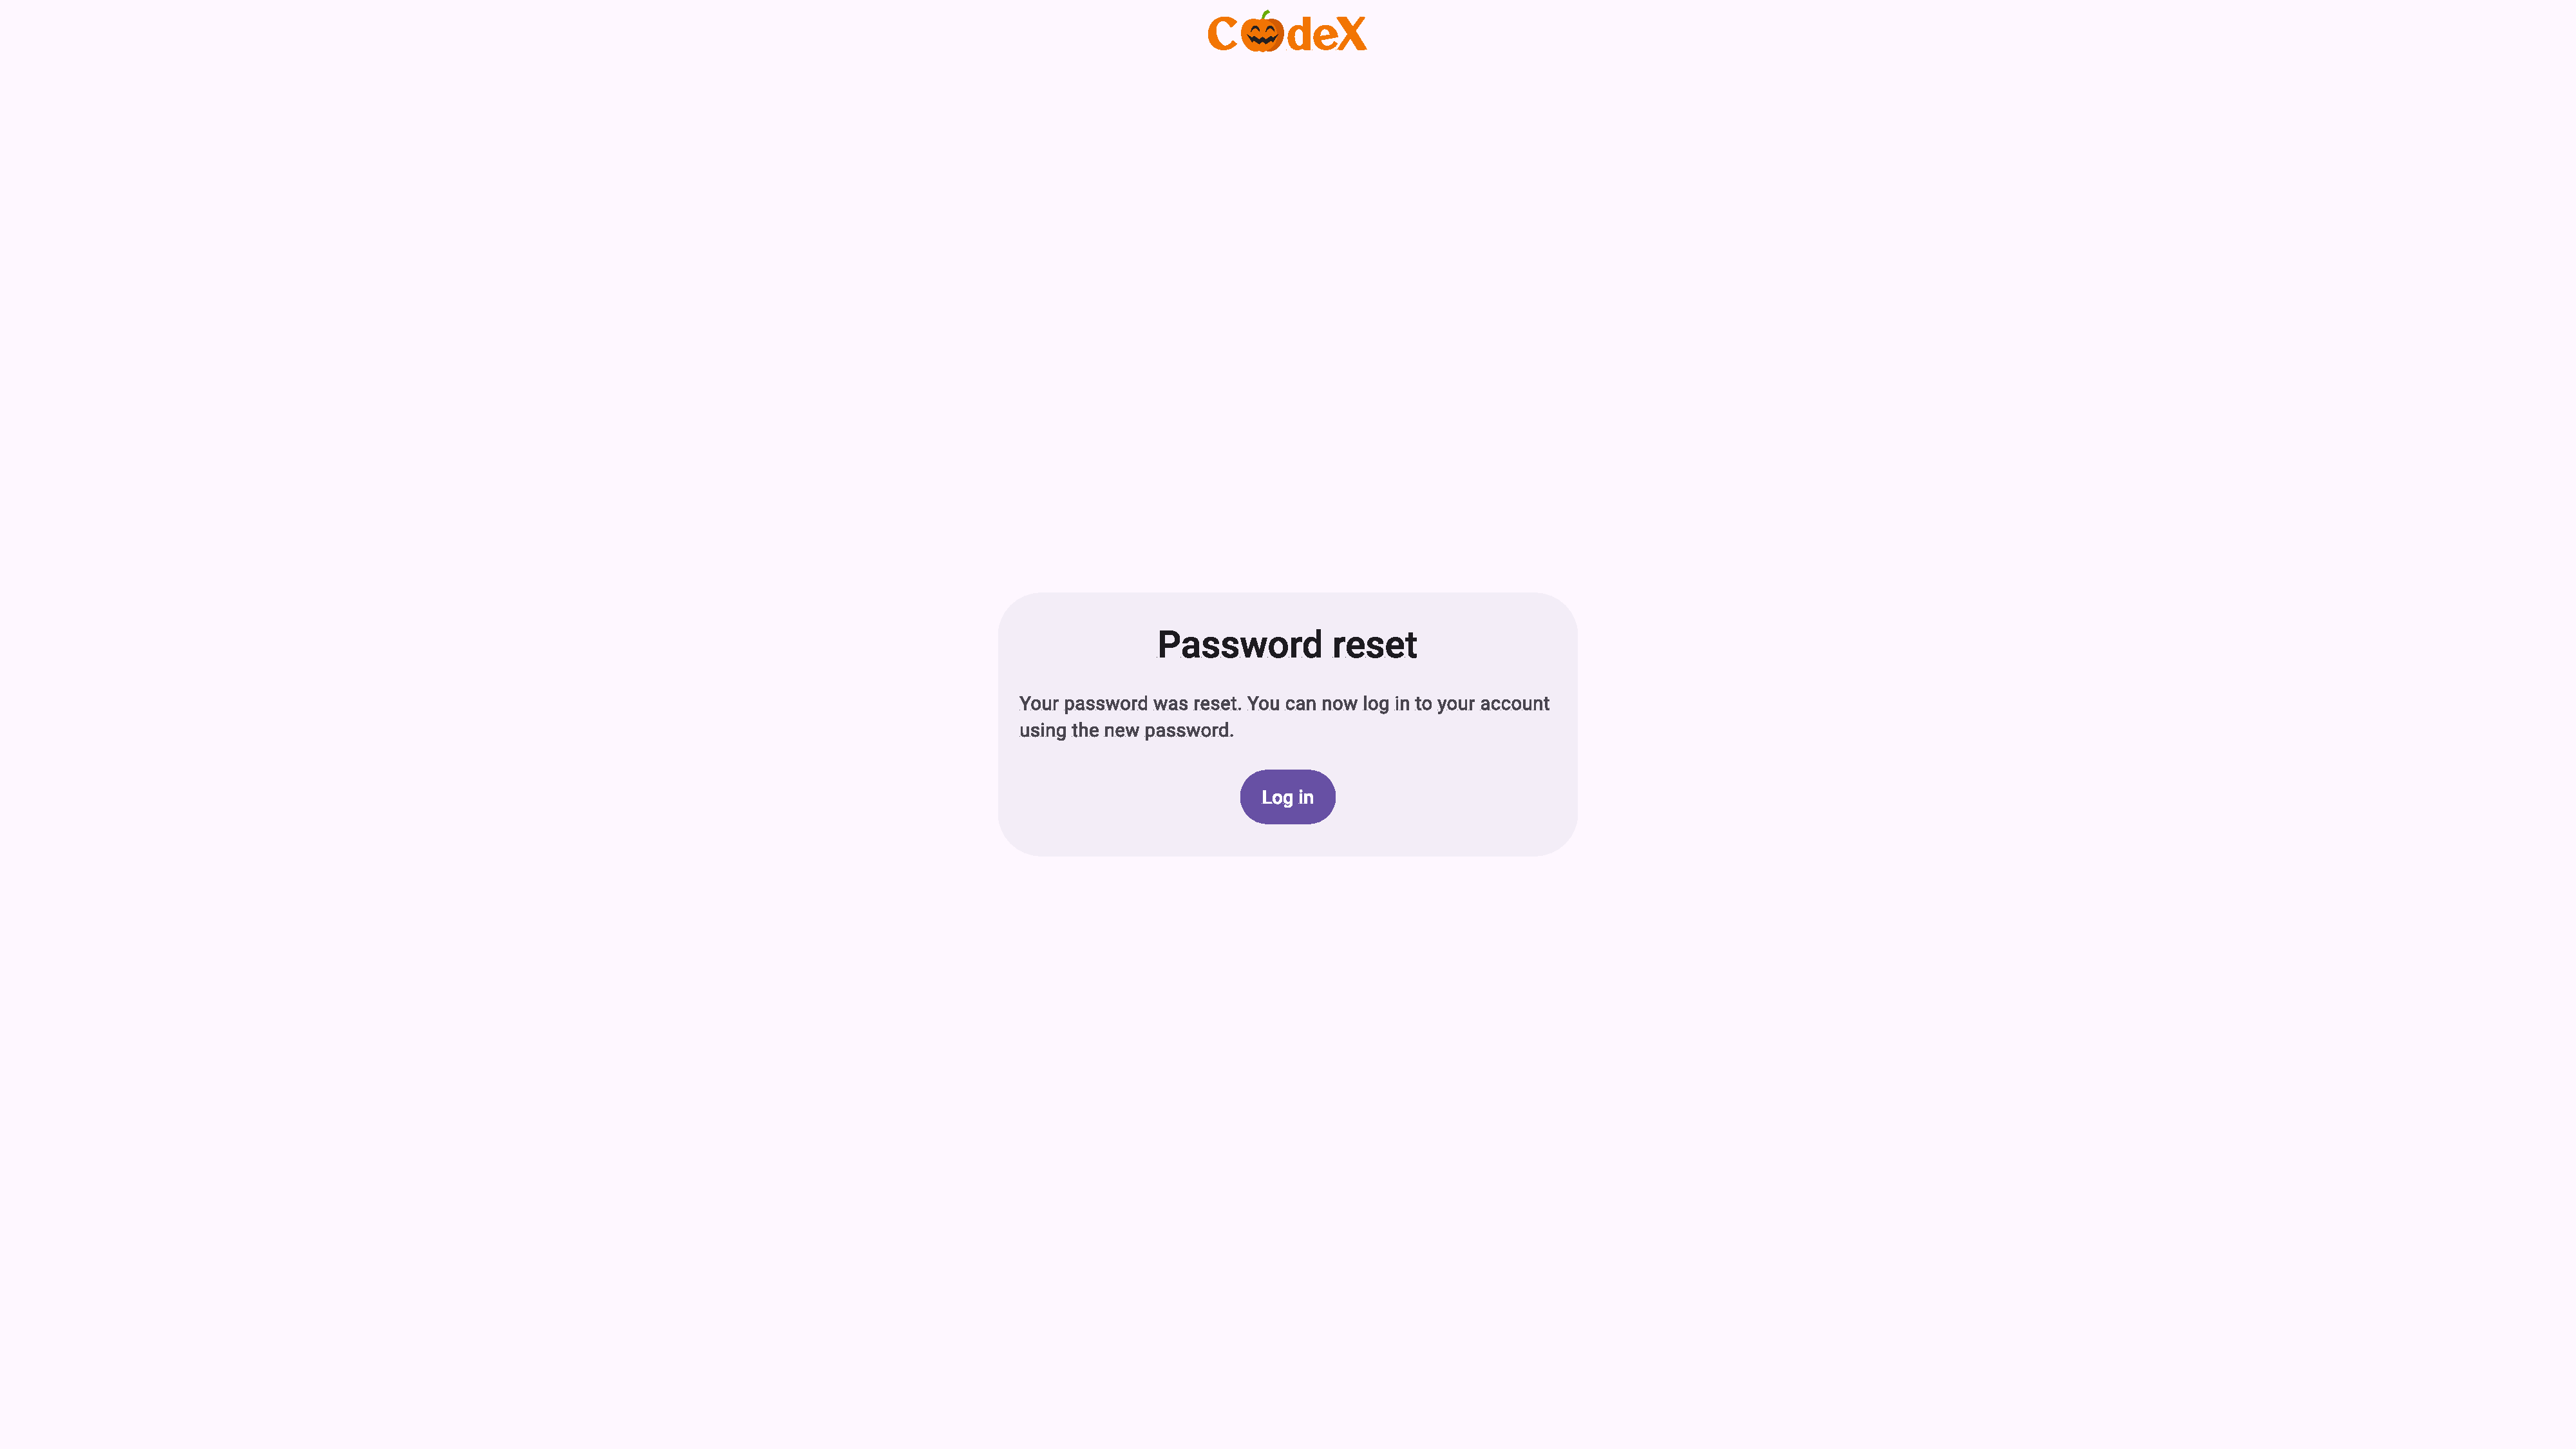
\includegraphics[width=\linewidth]{figures/ui/desktop/Reset_Password_Screen resetted}
    \caption{\hyperref[abr:GUI]{GUI}: Reset password screen after the password was set}
    \label{fig:ui-d-reset-password-reset}
\end{figure}
\begin{figure}
    \centering
    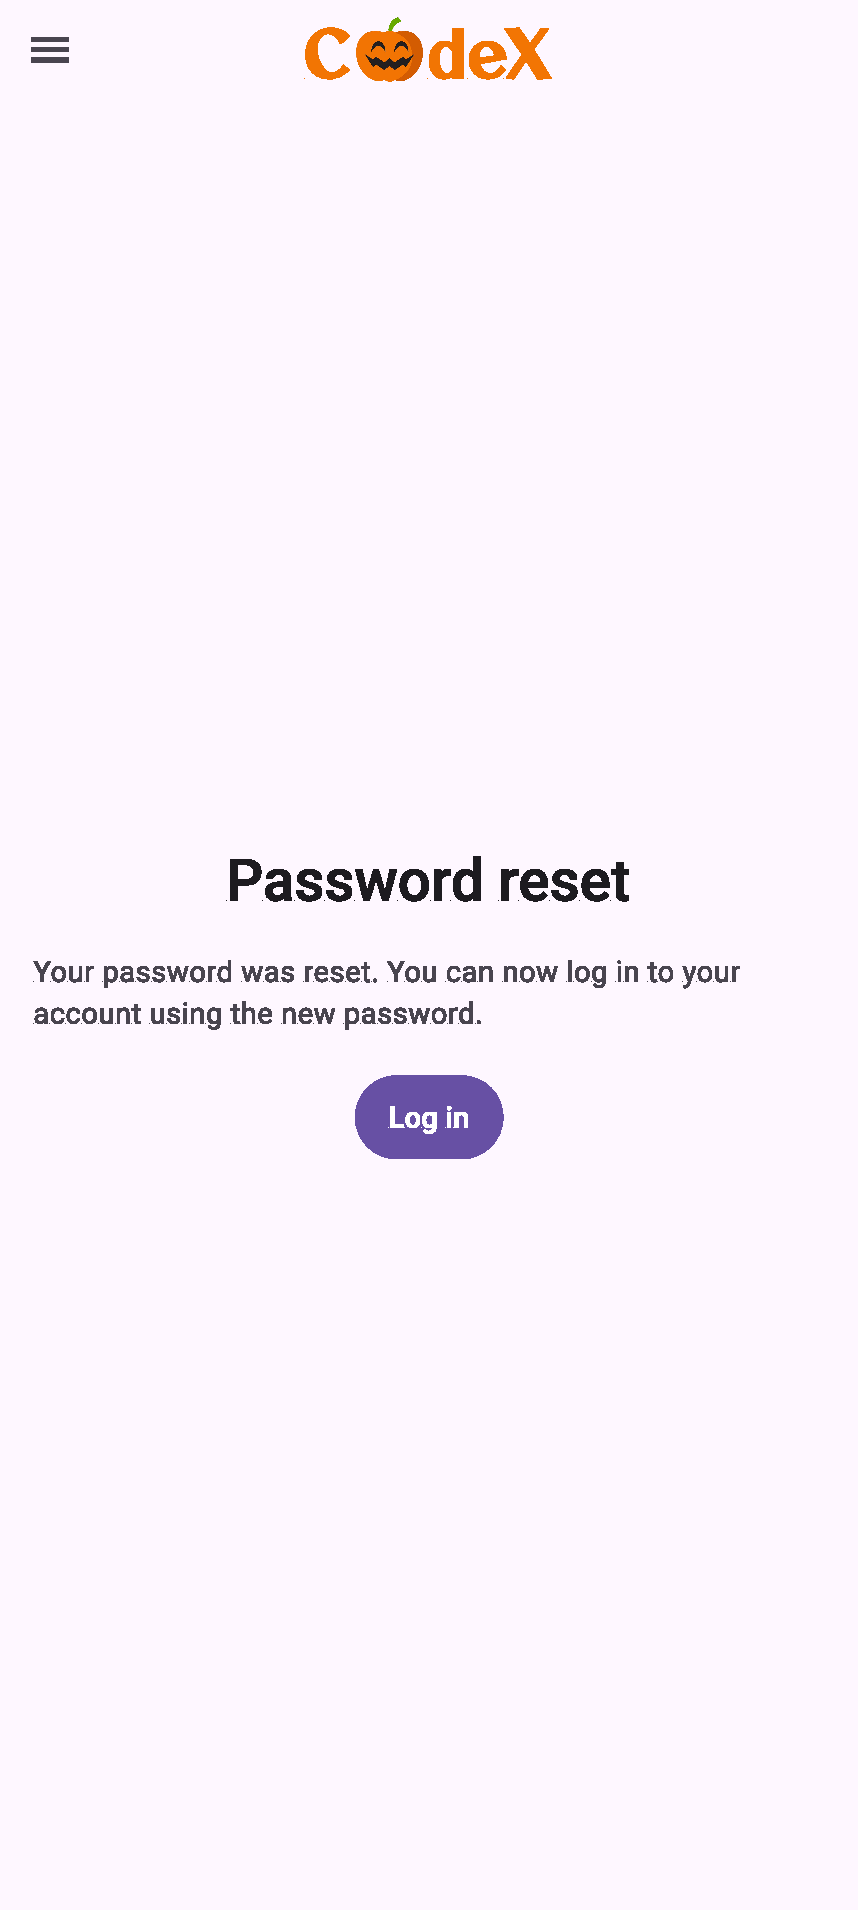
\includegraphics[width=5cm]{figures/ui/mobile/Reset_Password_Screen resetted}
    \caption{\hyperref[abr:GUI]{GUI}: Reset password screen after the password was set (mobile)}
    \label{fig:ui-m-reset-password-reset}
\end{figure}

\subsection{Signup}
The signup screen (\ref{fig:ui-d-signup}/\ref{fig:ui-m-signup}) allows a user to create a new account by entering email, username and a password. \newline
The screen also provides options to log in instead, or to use an \textit{\hyperref[def:oauth]{OAuth} provider}.
\begin{figure}
    \centering
    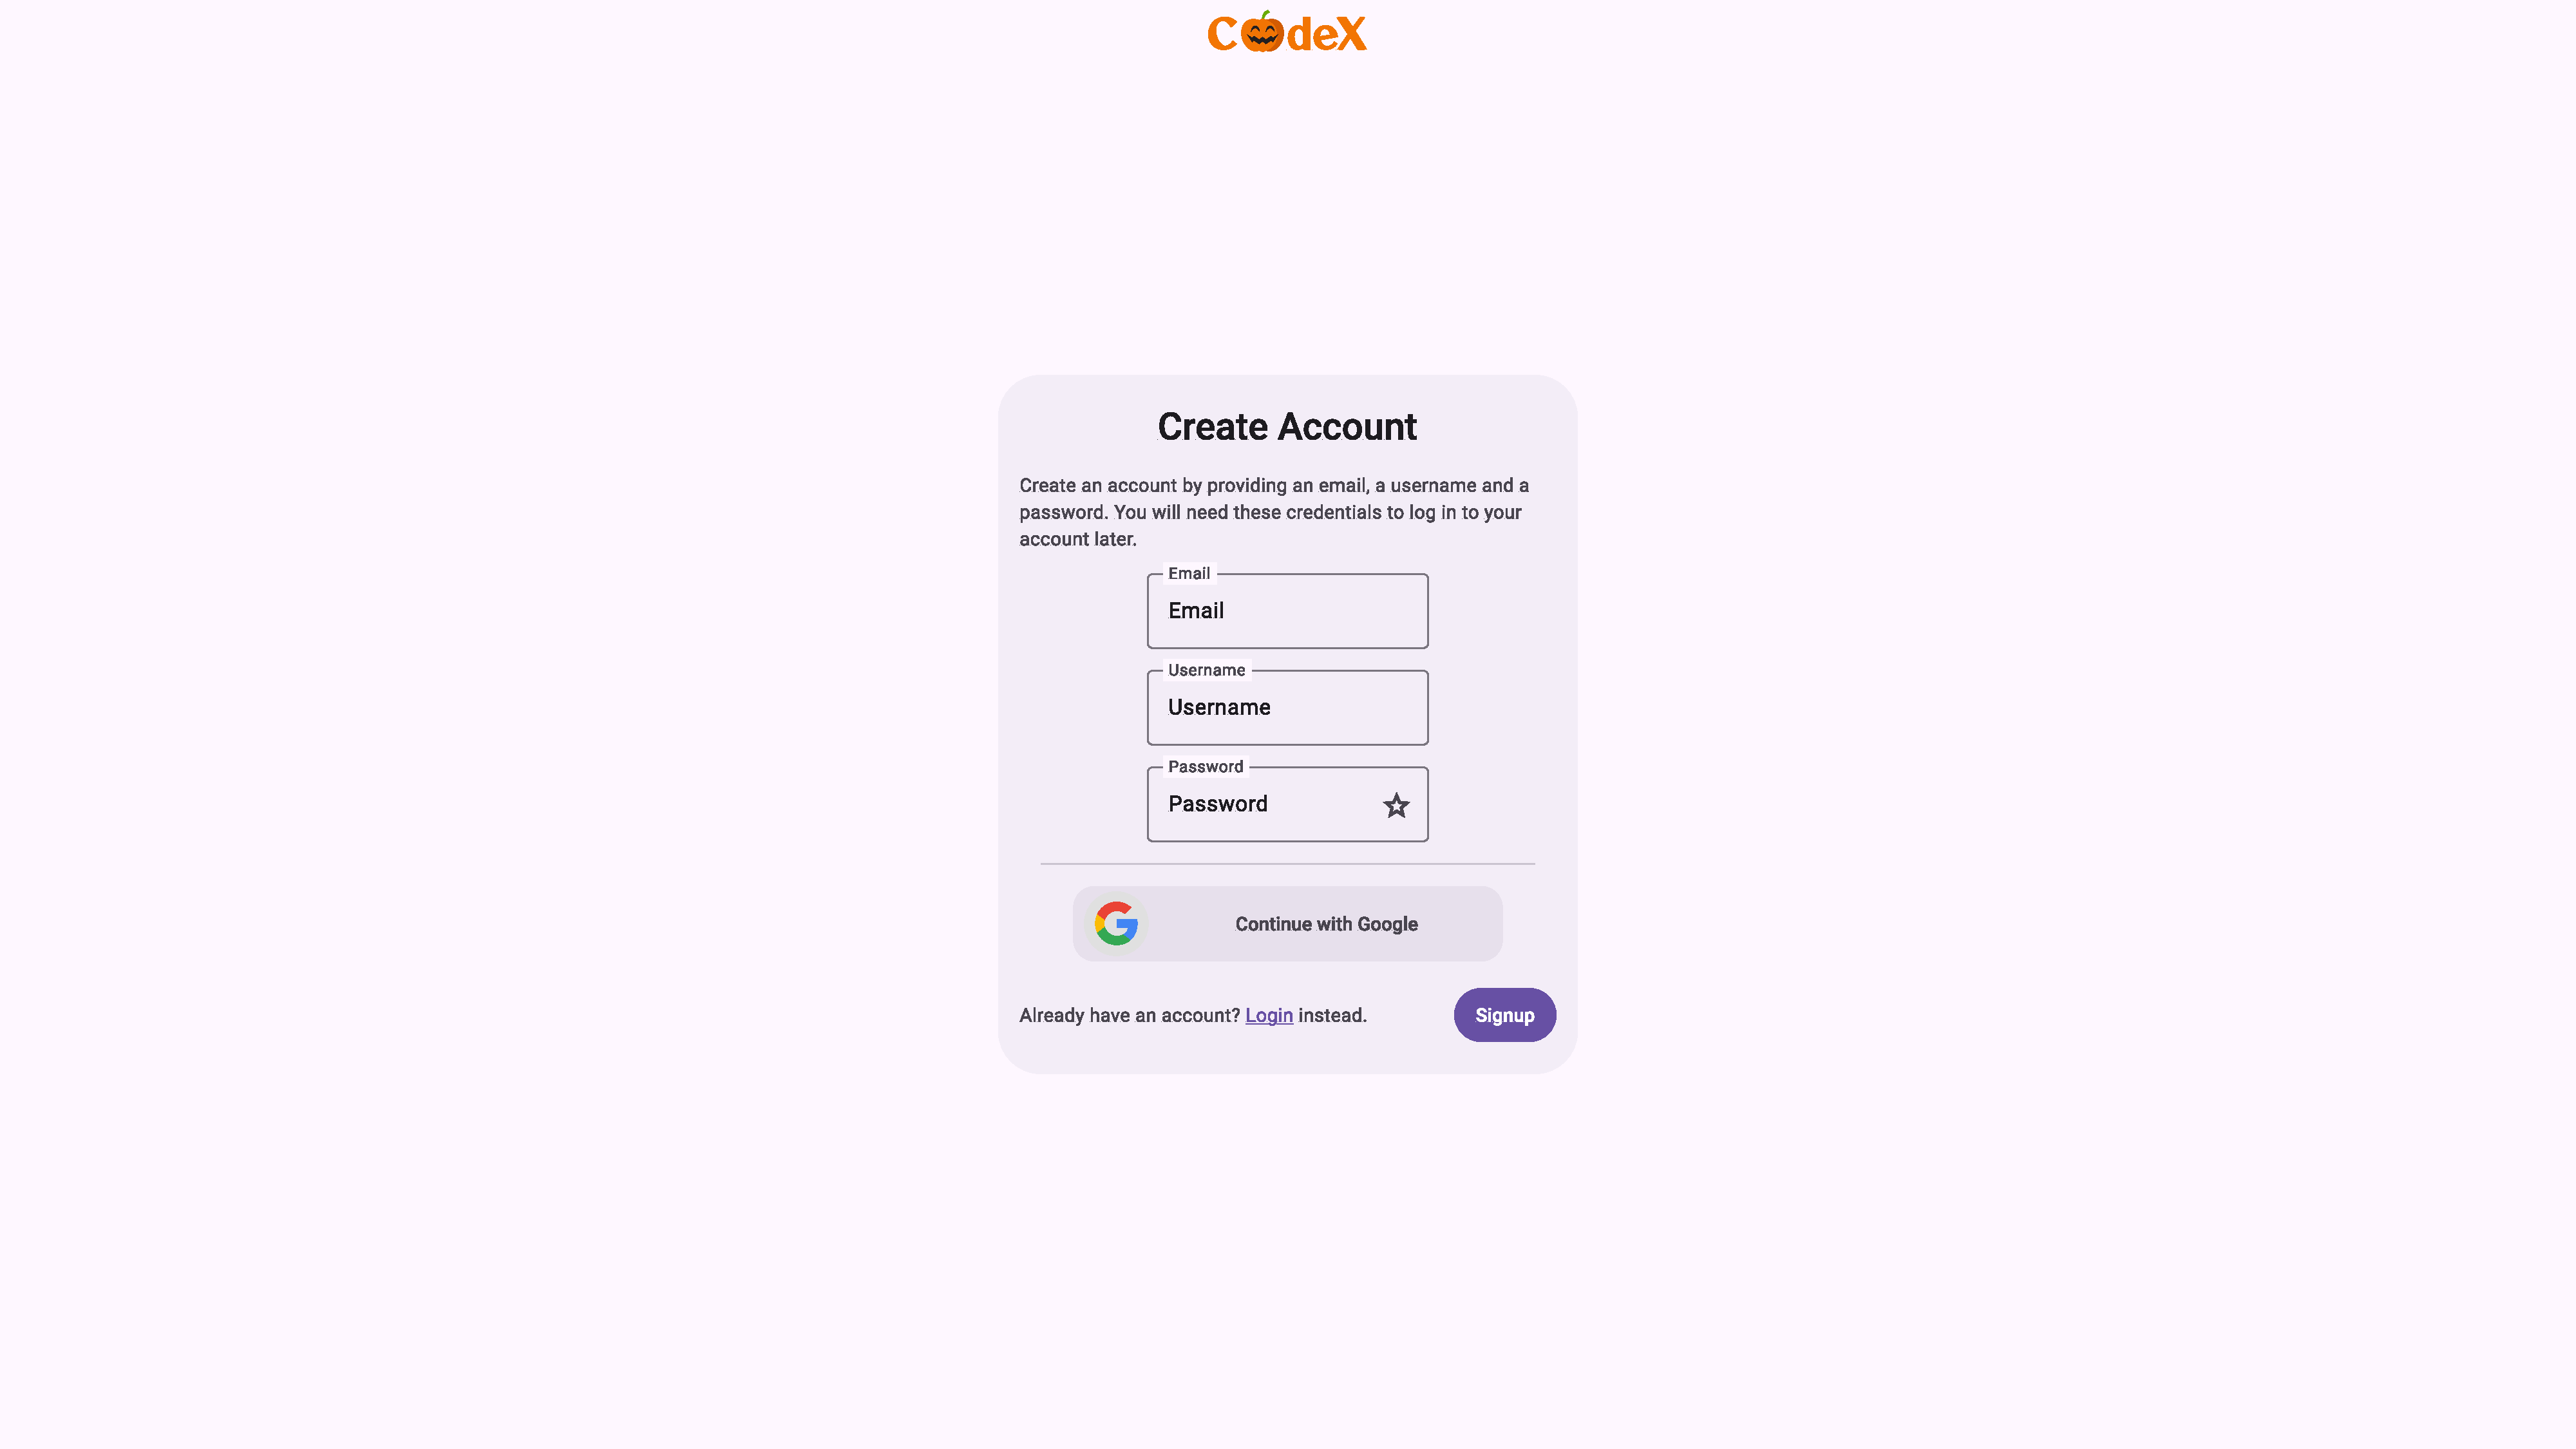
\includegraphics[width=\linewidth]{figures/ui/desktop/Signup_Screen}
    \caption{\hyperref[abr:GUI]{GUI}: Signup screen}
    \label{fig:ui-d-signup}
\end{figure}
\begin{figure}
    \centering
    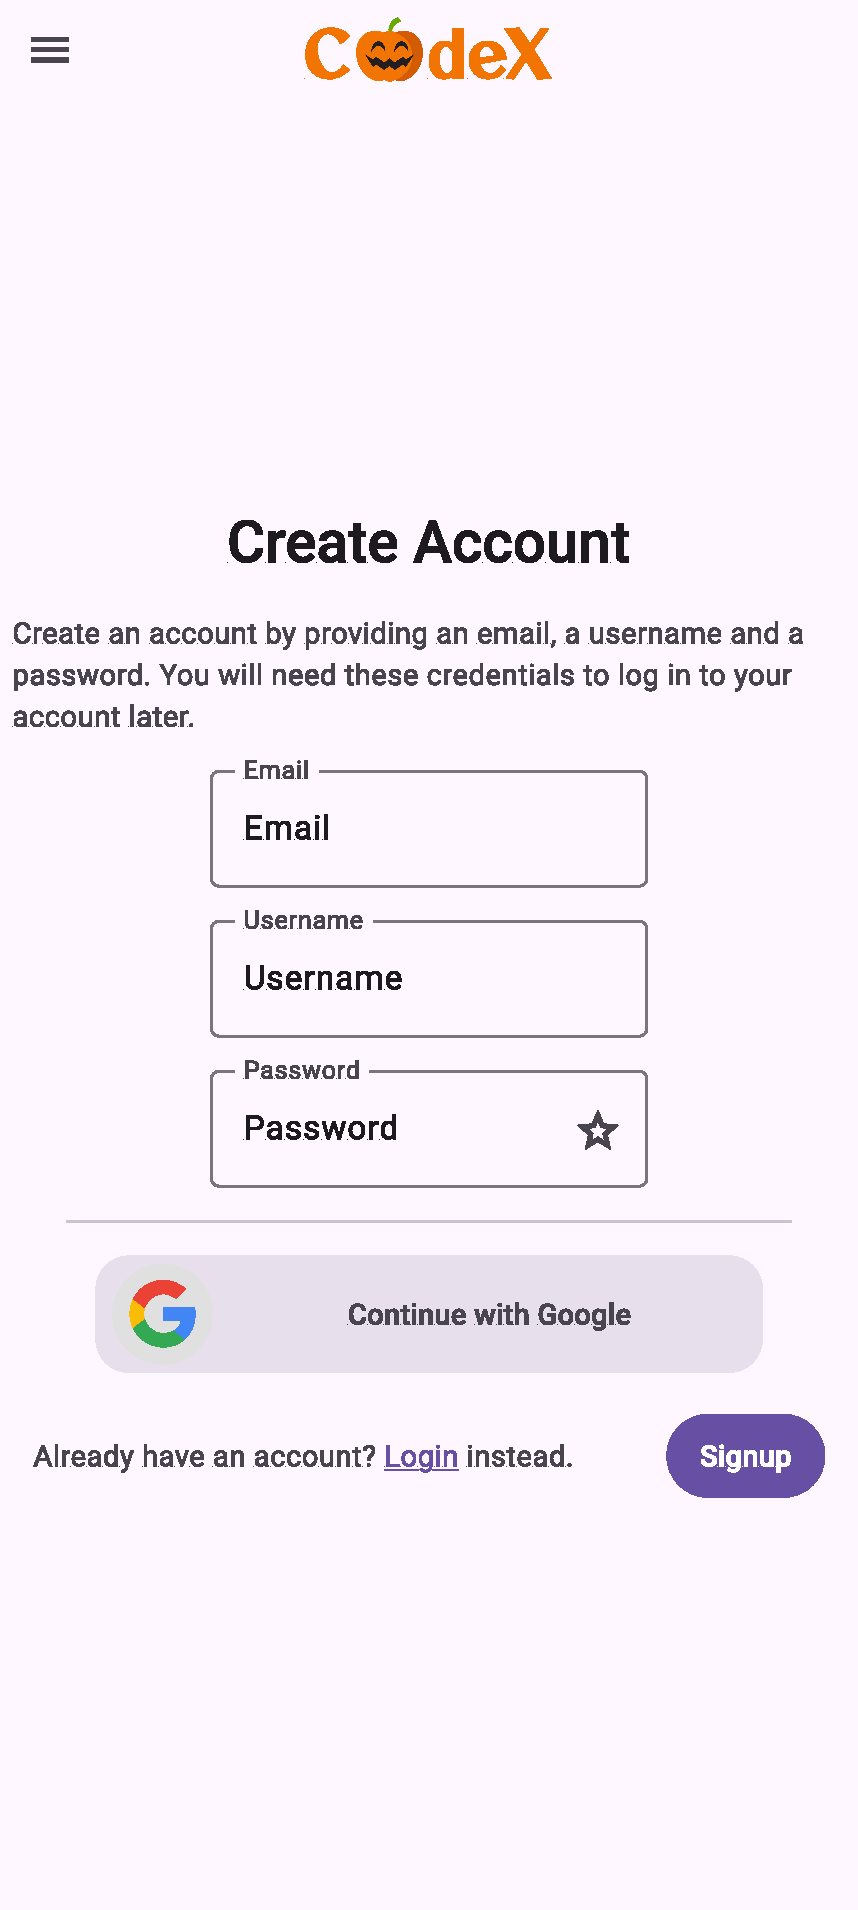
\includegraphics[width=5cm]{figures/ui/mobile/Signup_Screen}
    \caption{\hyperref[abr:GUI]{GUI}: Signup screen (mobile)}
    \label{fig:ui-m-signup}
\end{figure}

\subsection{Not verified screen}
The not verified screen is shown to authenticated users that try to perform an action that requires their email to be verified. \newline
Users have the option to request a verification message (\ref{fig:ui-d-not-verified-initial}/\ref{fig:ui-m-not-verified-initial}), after which an informative message is shown (\ref{fig:ui-d-not-verified-requested}/\ref{fig:ui-m-not-verified-requested}).
\begin{figure}
    \centering
    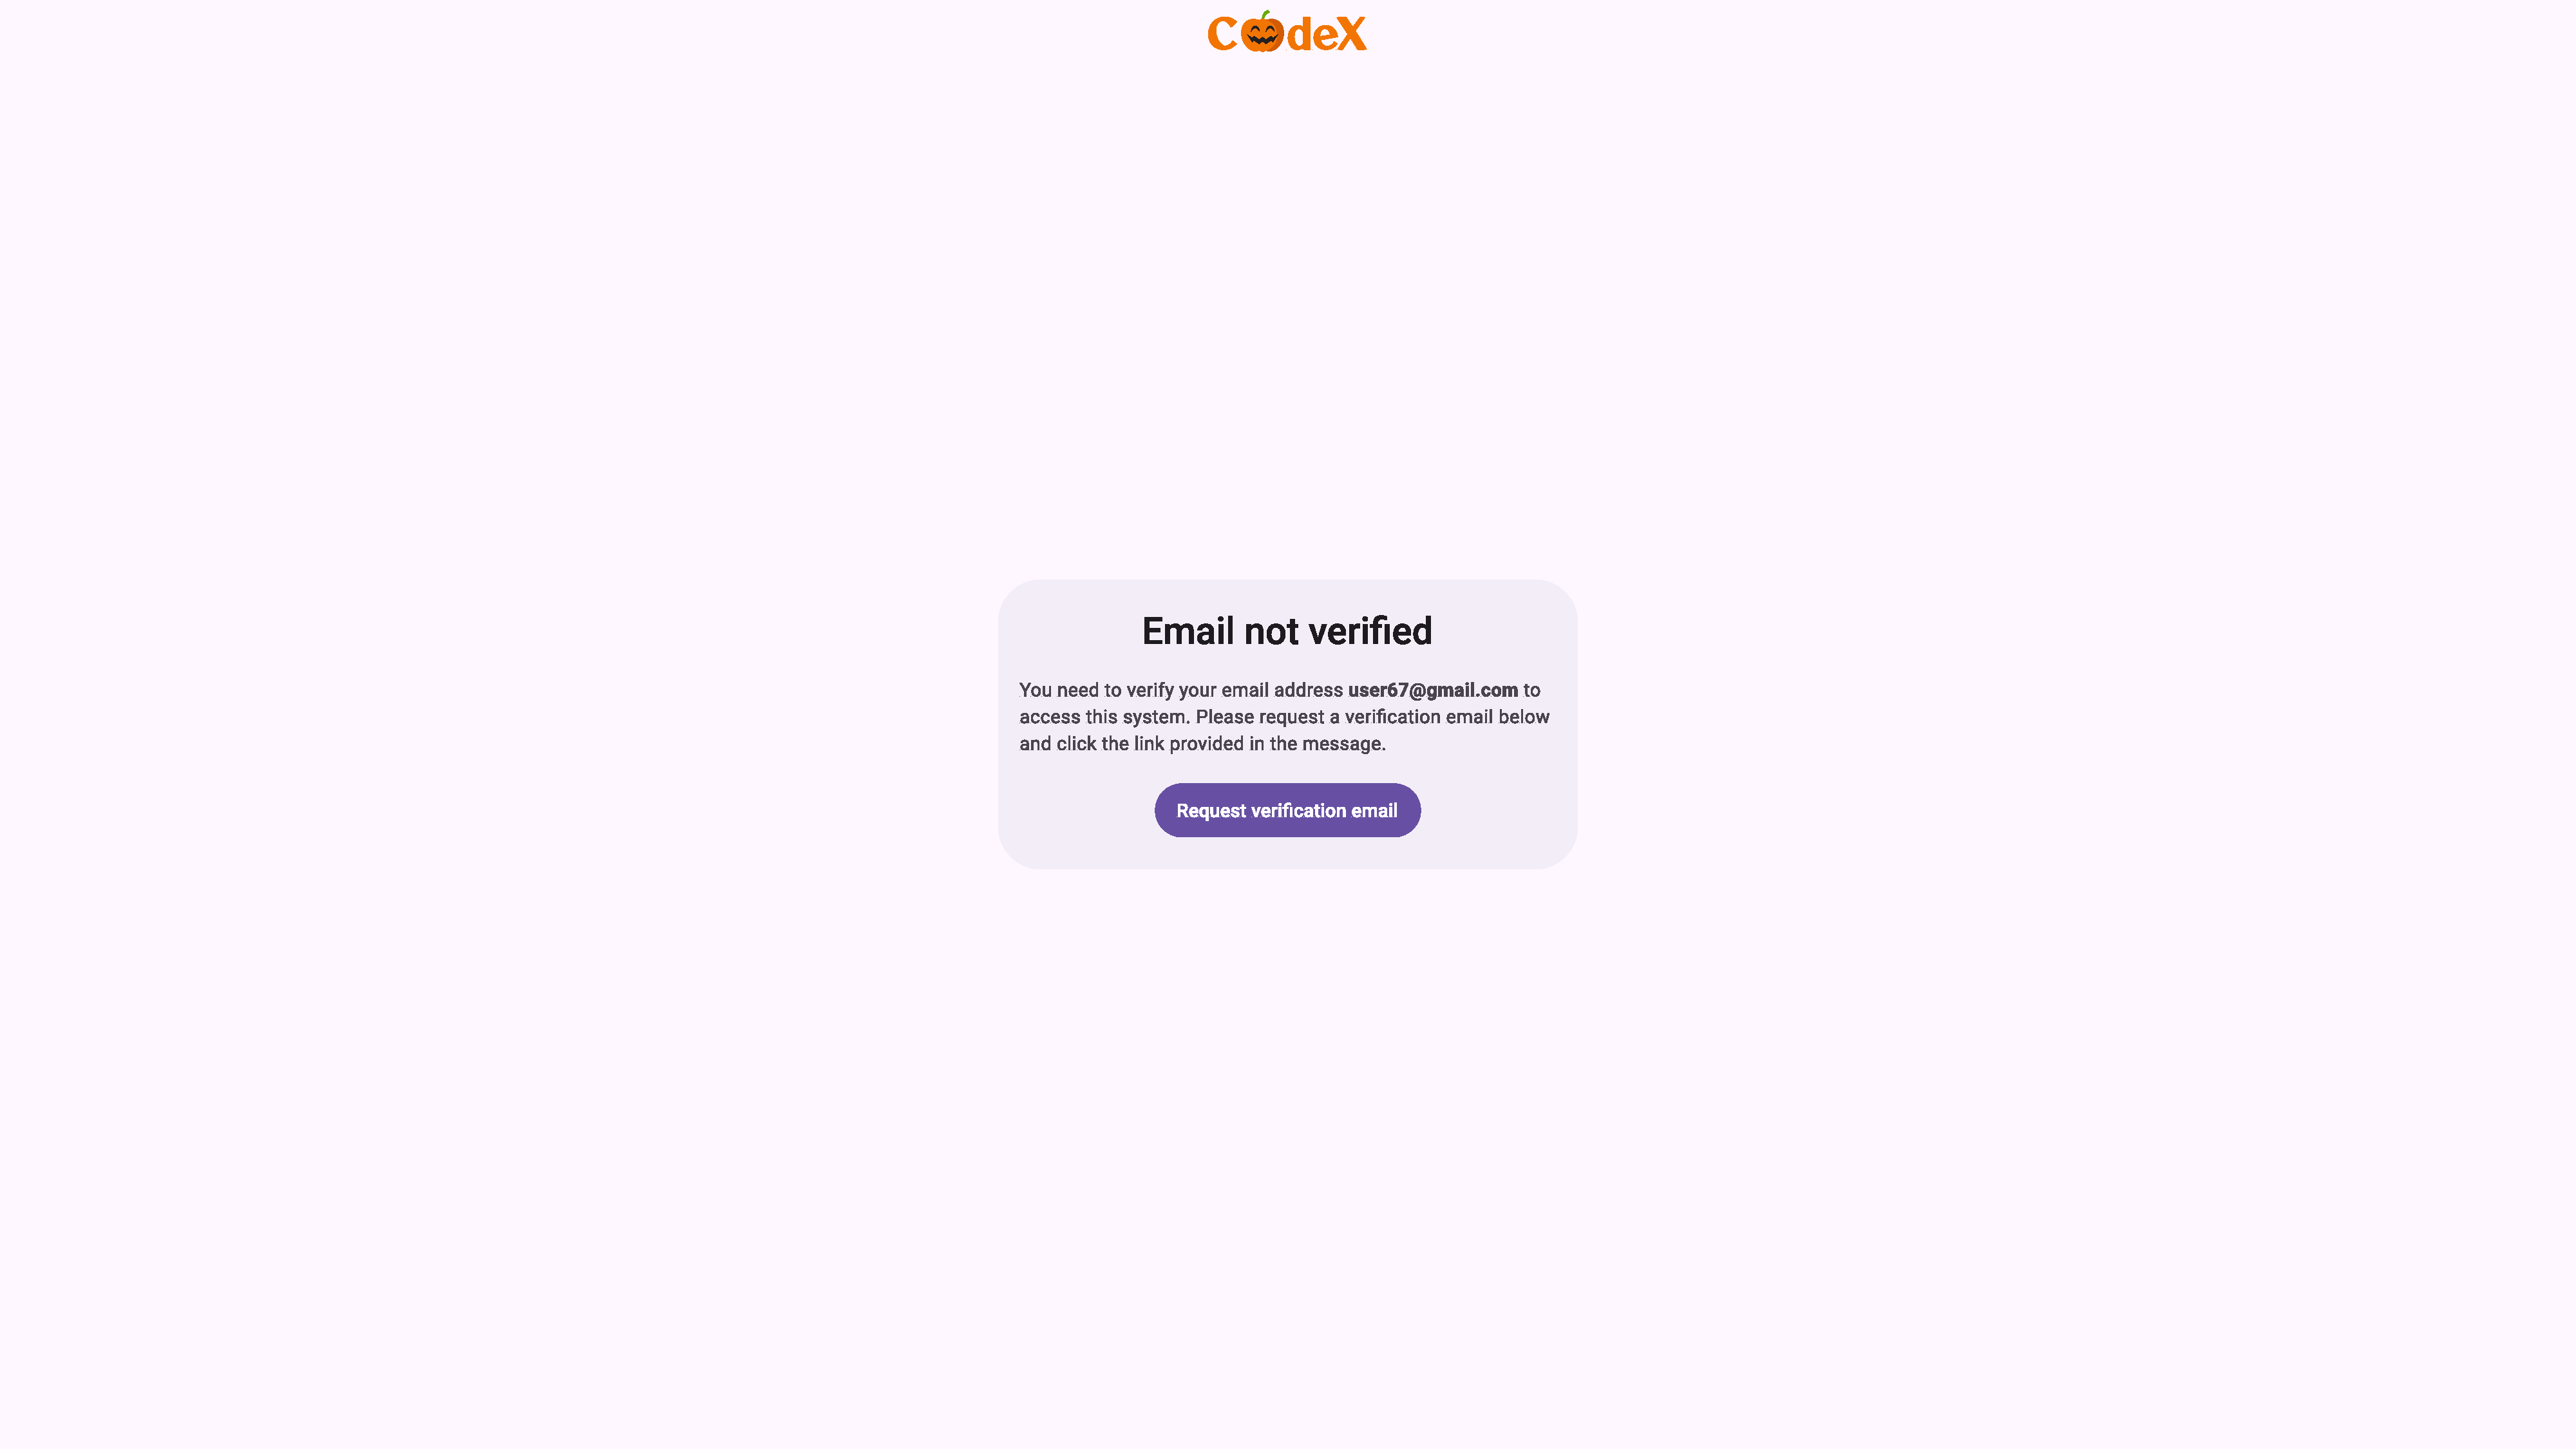
\includegraphics[width=\linewidth]{figures/ui/desktop/Not_Verified_Screen initial}
    \caption{\hyperref[abr:GUI]{GUI}: Not verified screen}
    \label{fig:ui-d-not-verified-initial}
\end{figure}
\begin{figure}
    \centering
    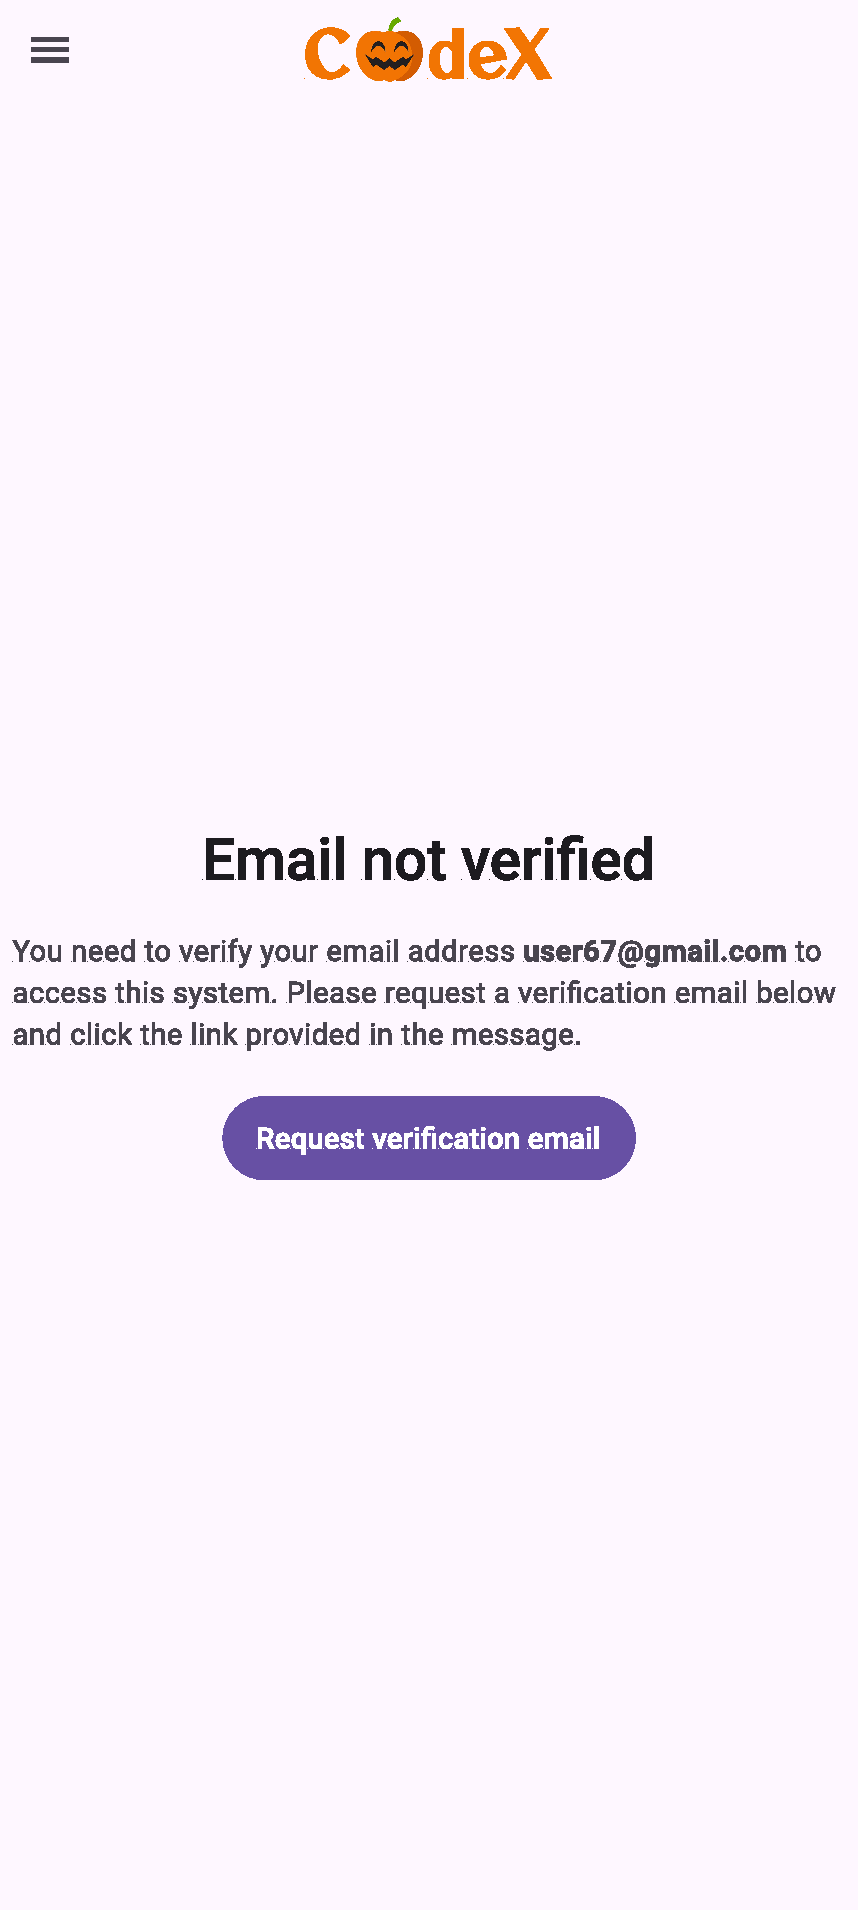
\includegraphics[width=5cm]{figures/ui/mobile/Not_Verified_Screen initial}
    \caption{\hyperref[abr:GUI]{GUI}: Not verified screen (mobile)}
    \label{fig:ui-m-not-verified-initial}
\end{figure}

\begin{figure}
    \centering
    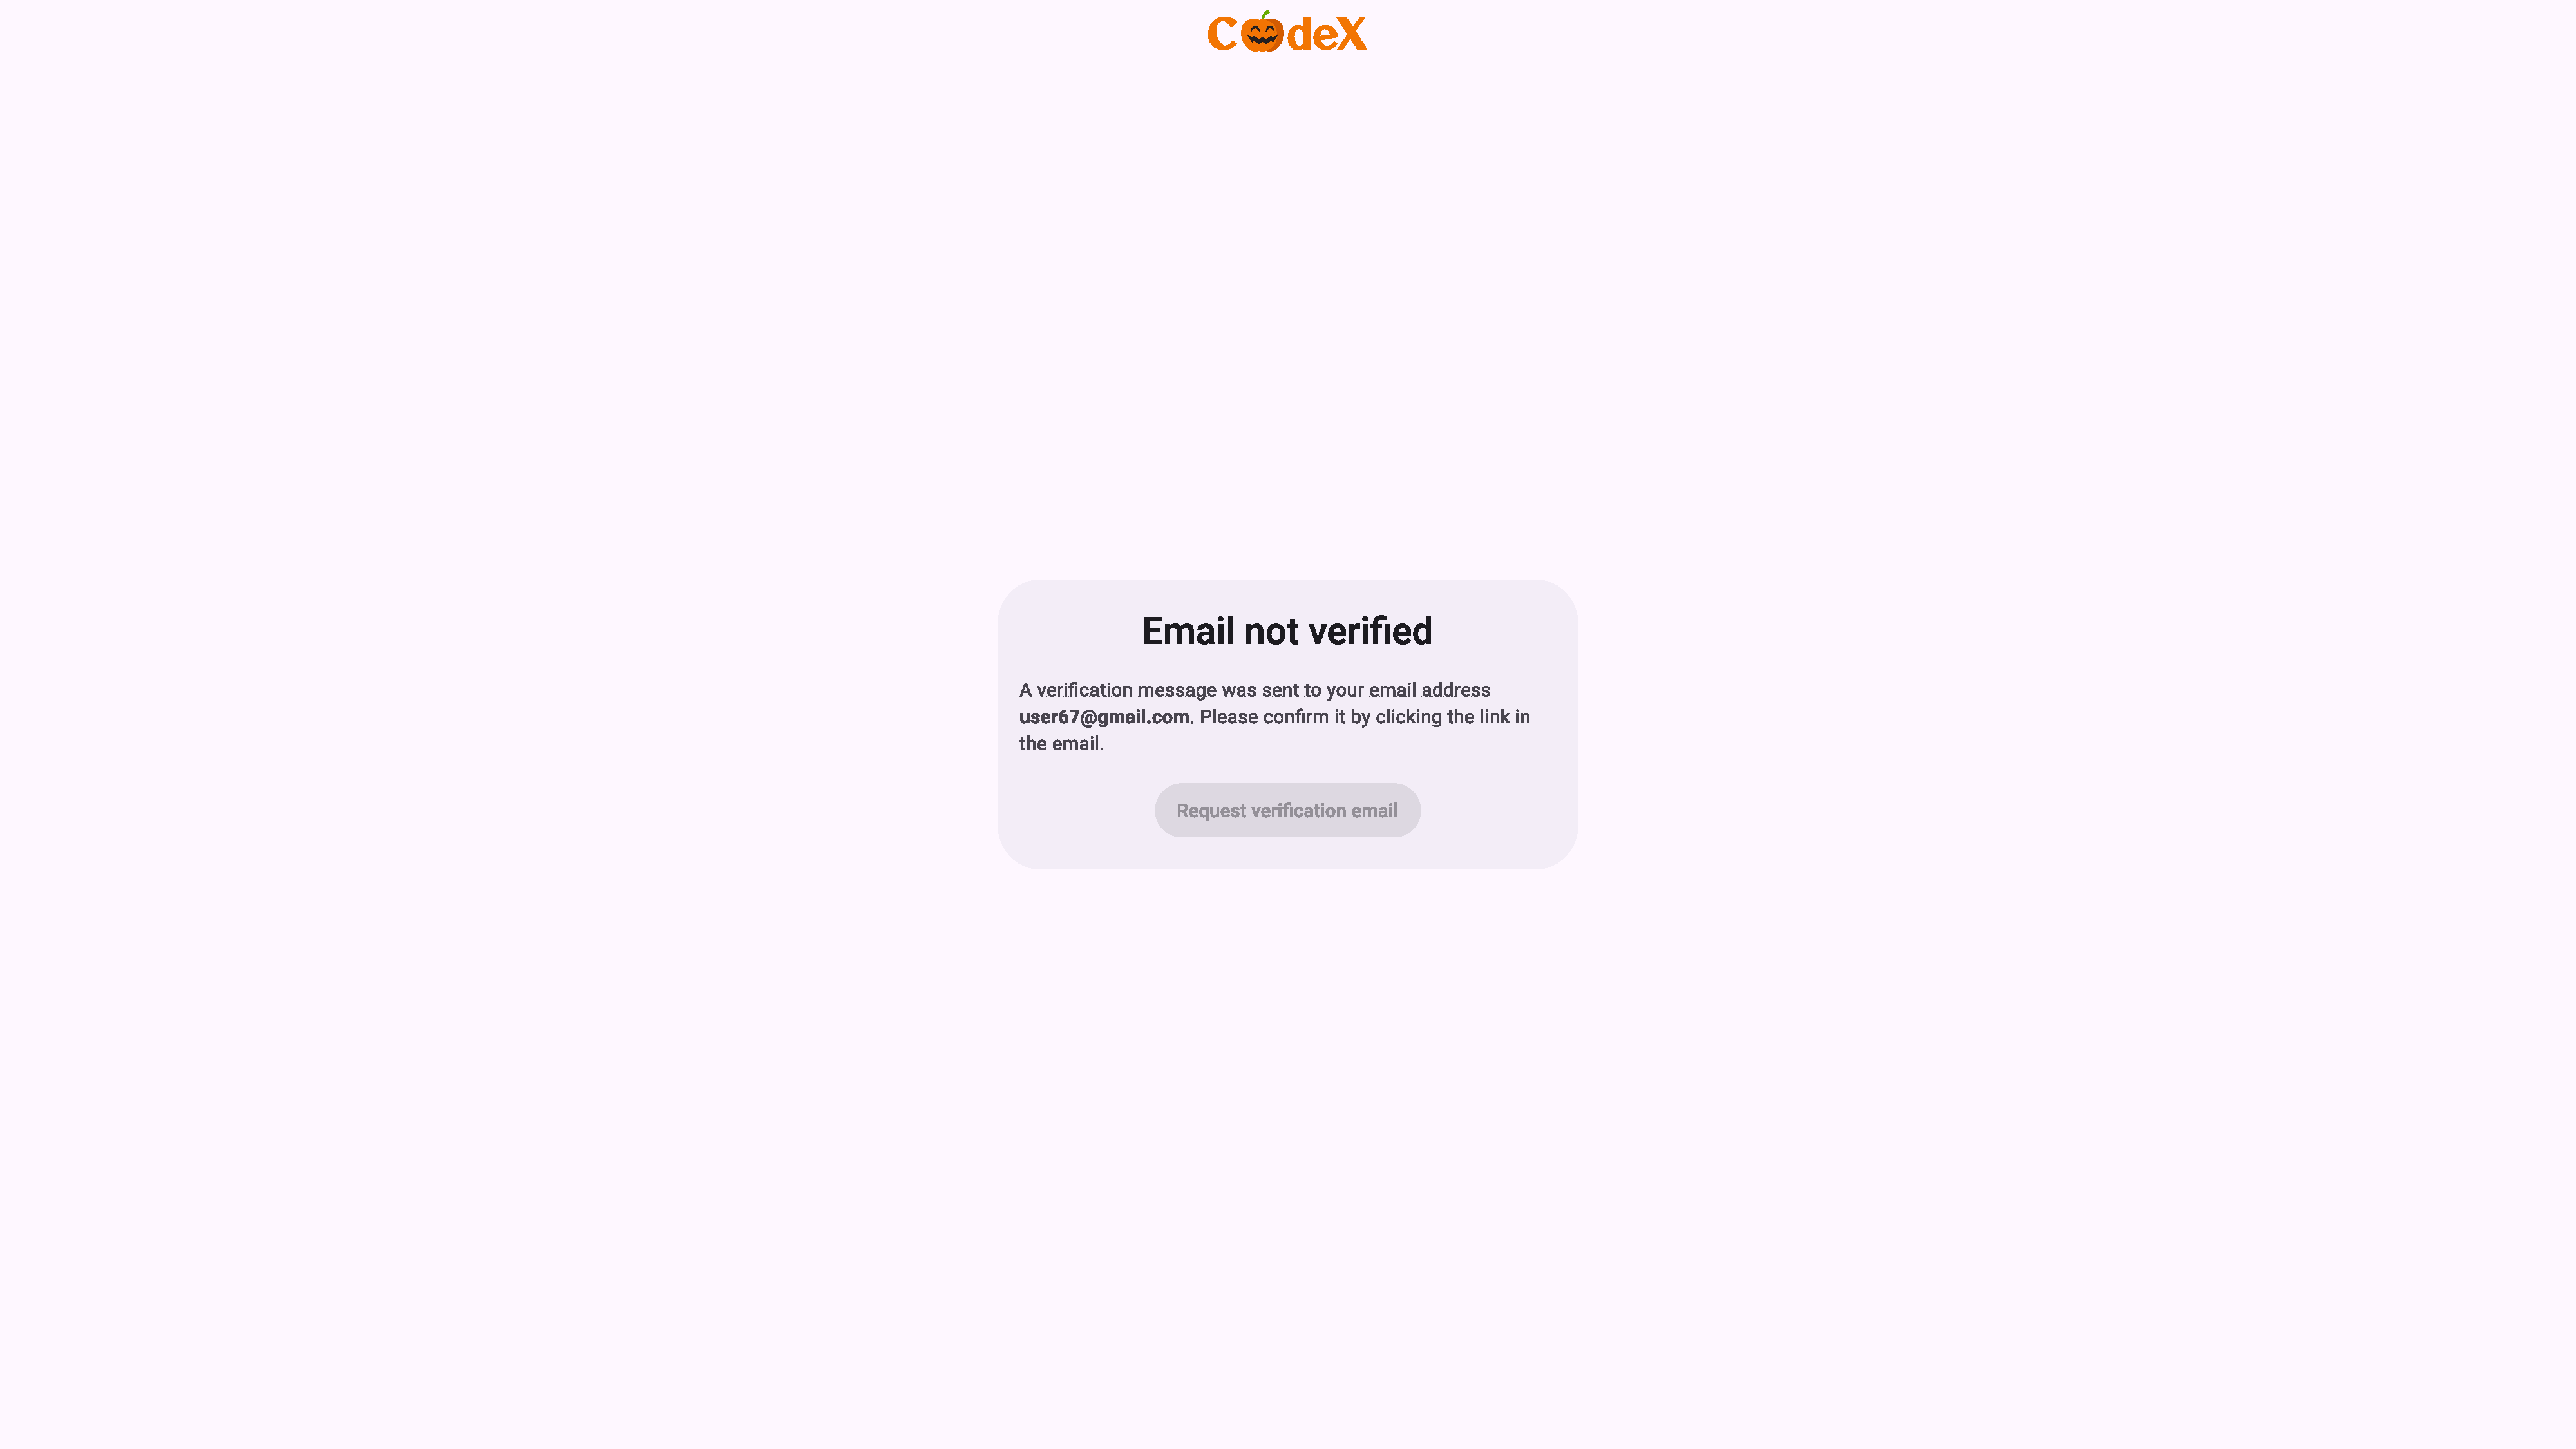
\includegraphics[width=\linewidth]{figures/ui/desktop/Not_Verified_Screen requested}
    \caption{\hyperref[abr:GUI]{GUI}: Not verified screen after requesting verification}
    \label{fig:ui-d-not-verified-requested}
\end{figure}
\begin{figure}
    \centering
    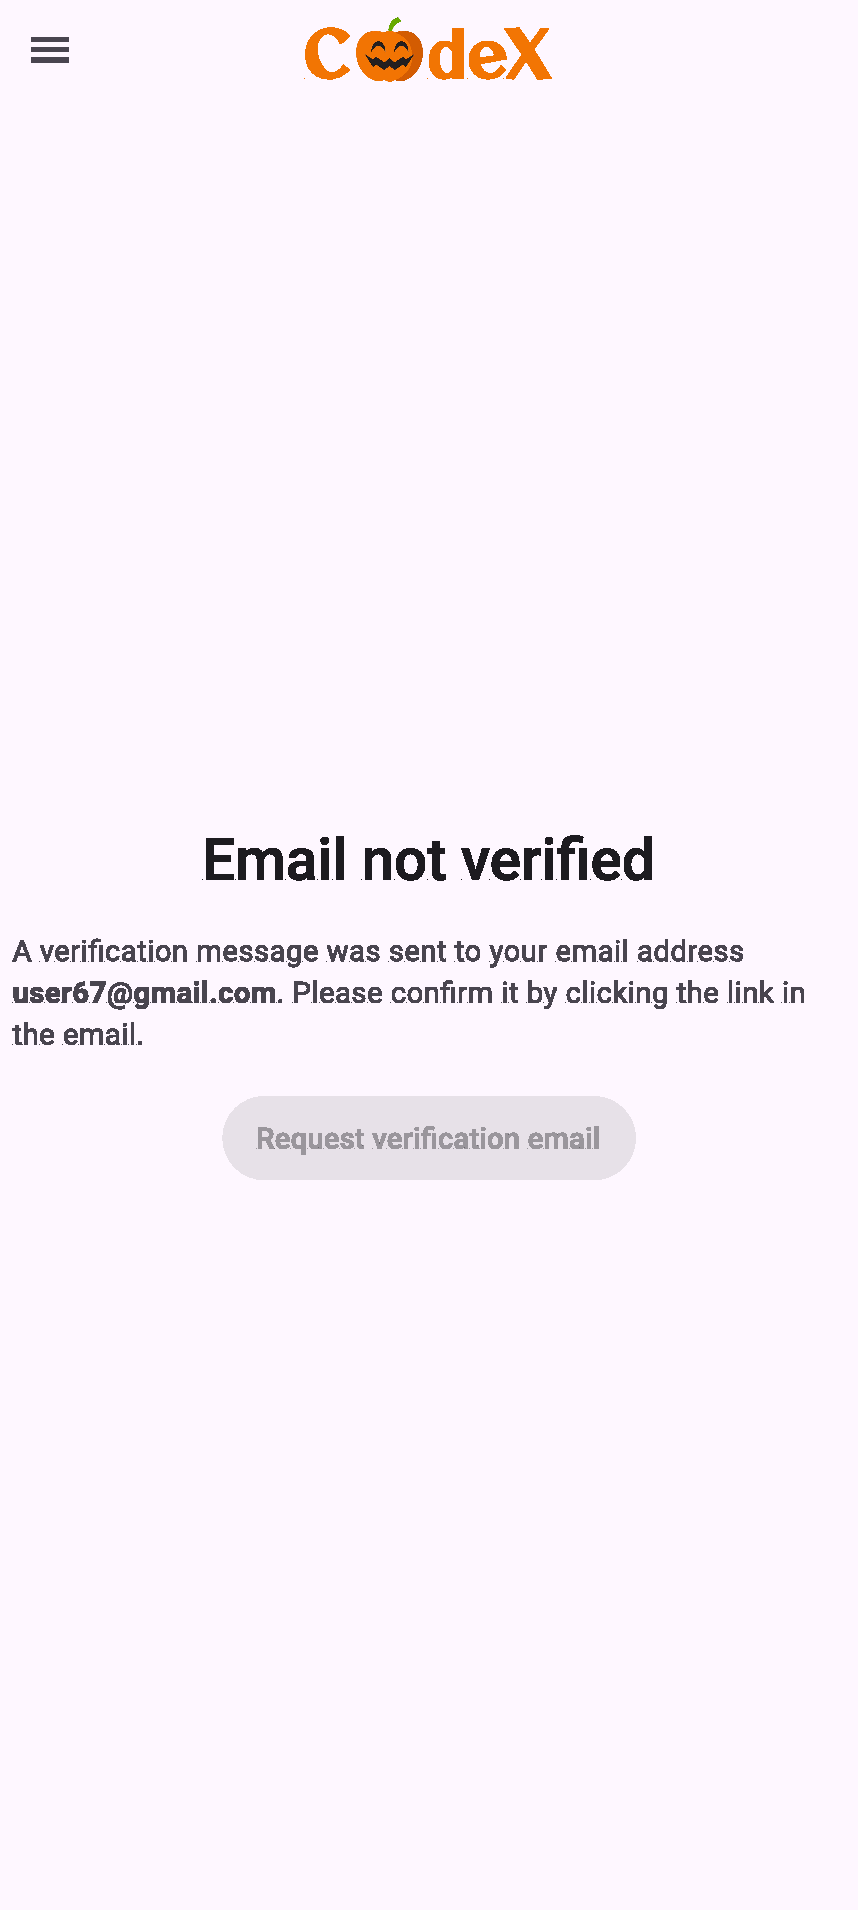
\includegraphics[width=5cm]{figures/ui/mobile/Not_Verified_Screen requested}
    \caption{\hyperref[abr:GUI]{GUI}: Not verified screen after requesting verification (mobile)}
    \label{fig:ui-m-not-verified-requested}
\end{figure}

\subsection{Verified screen}
The verified screen (\ref{fig:ui-d-verified}/\ref{fig:ui-m-verified}) is shown when the email of a user has been successfully verified.
This screen is shown after a user used the verification link in the message that was sent to them. \newline
\begin{figure}
    \centering
    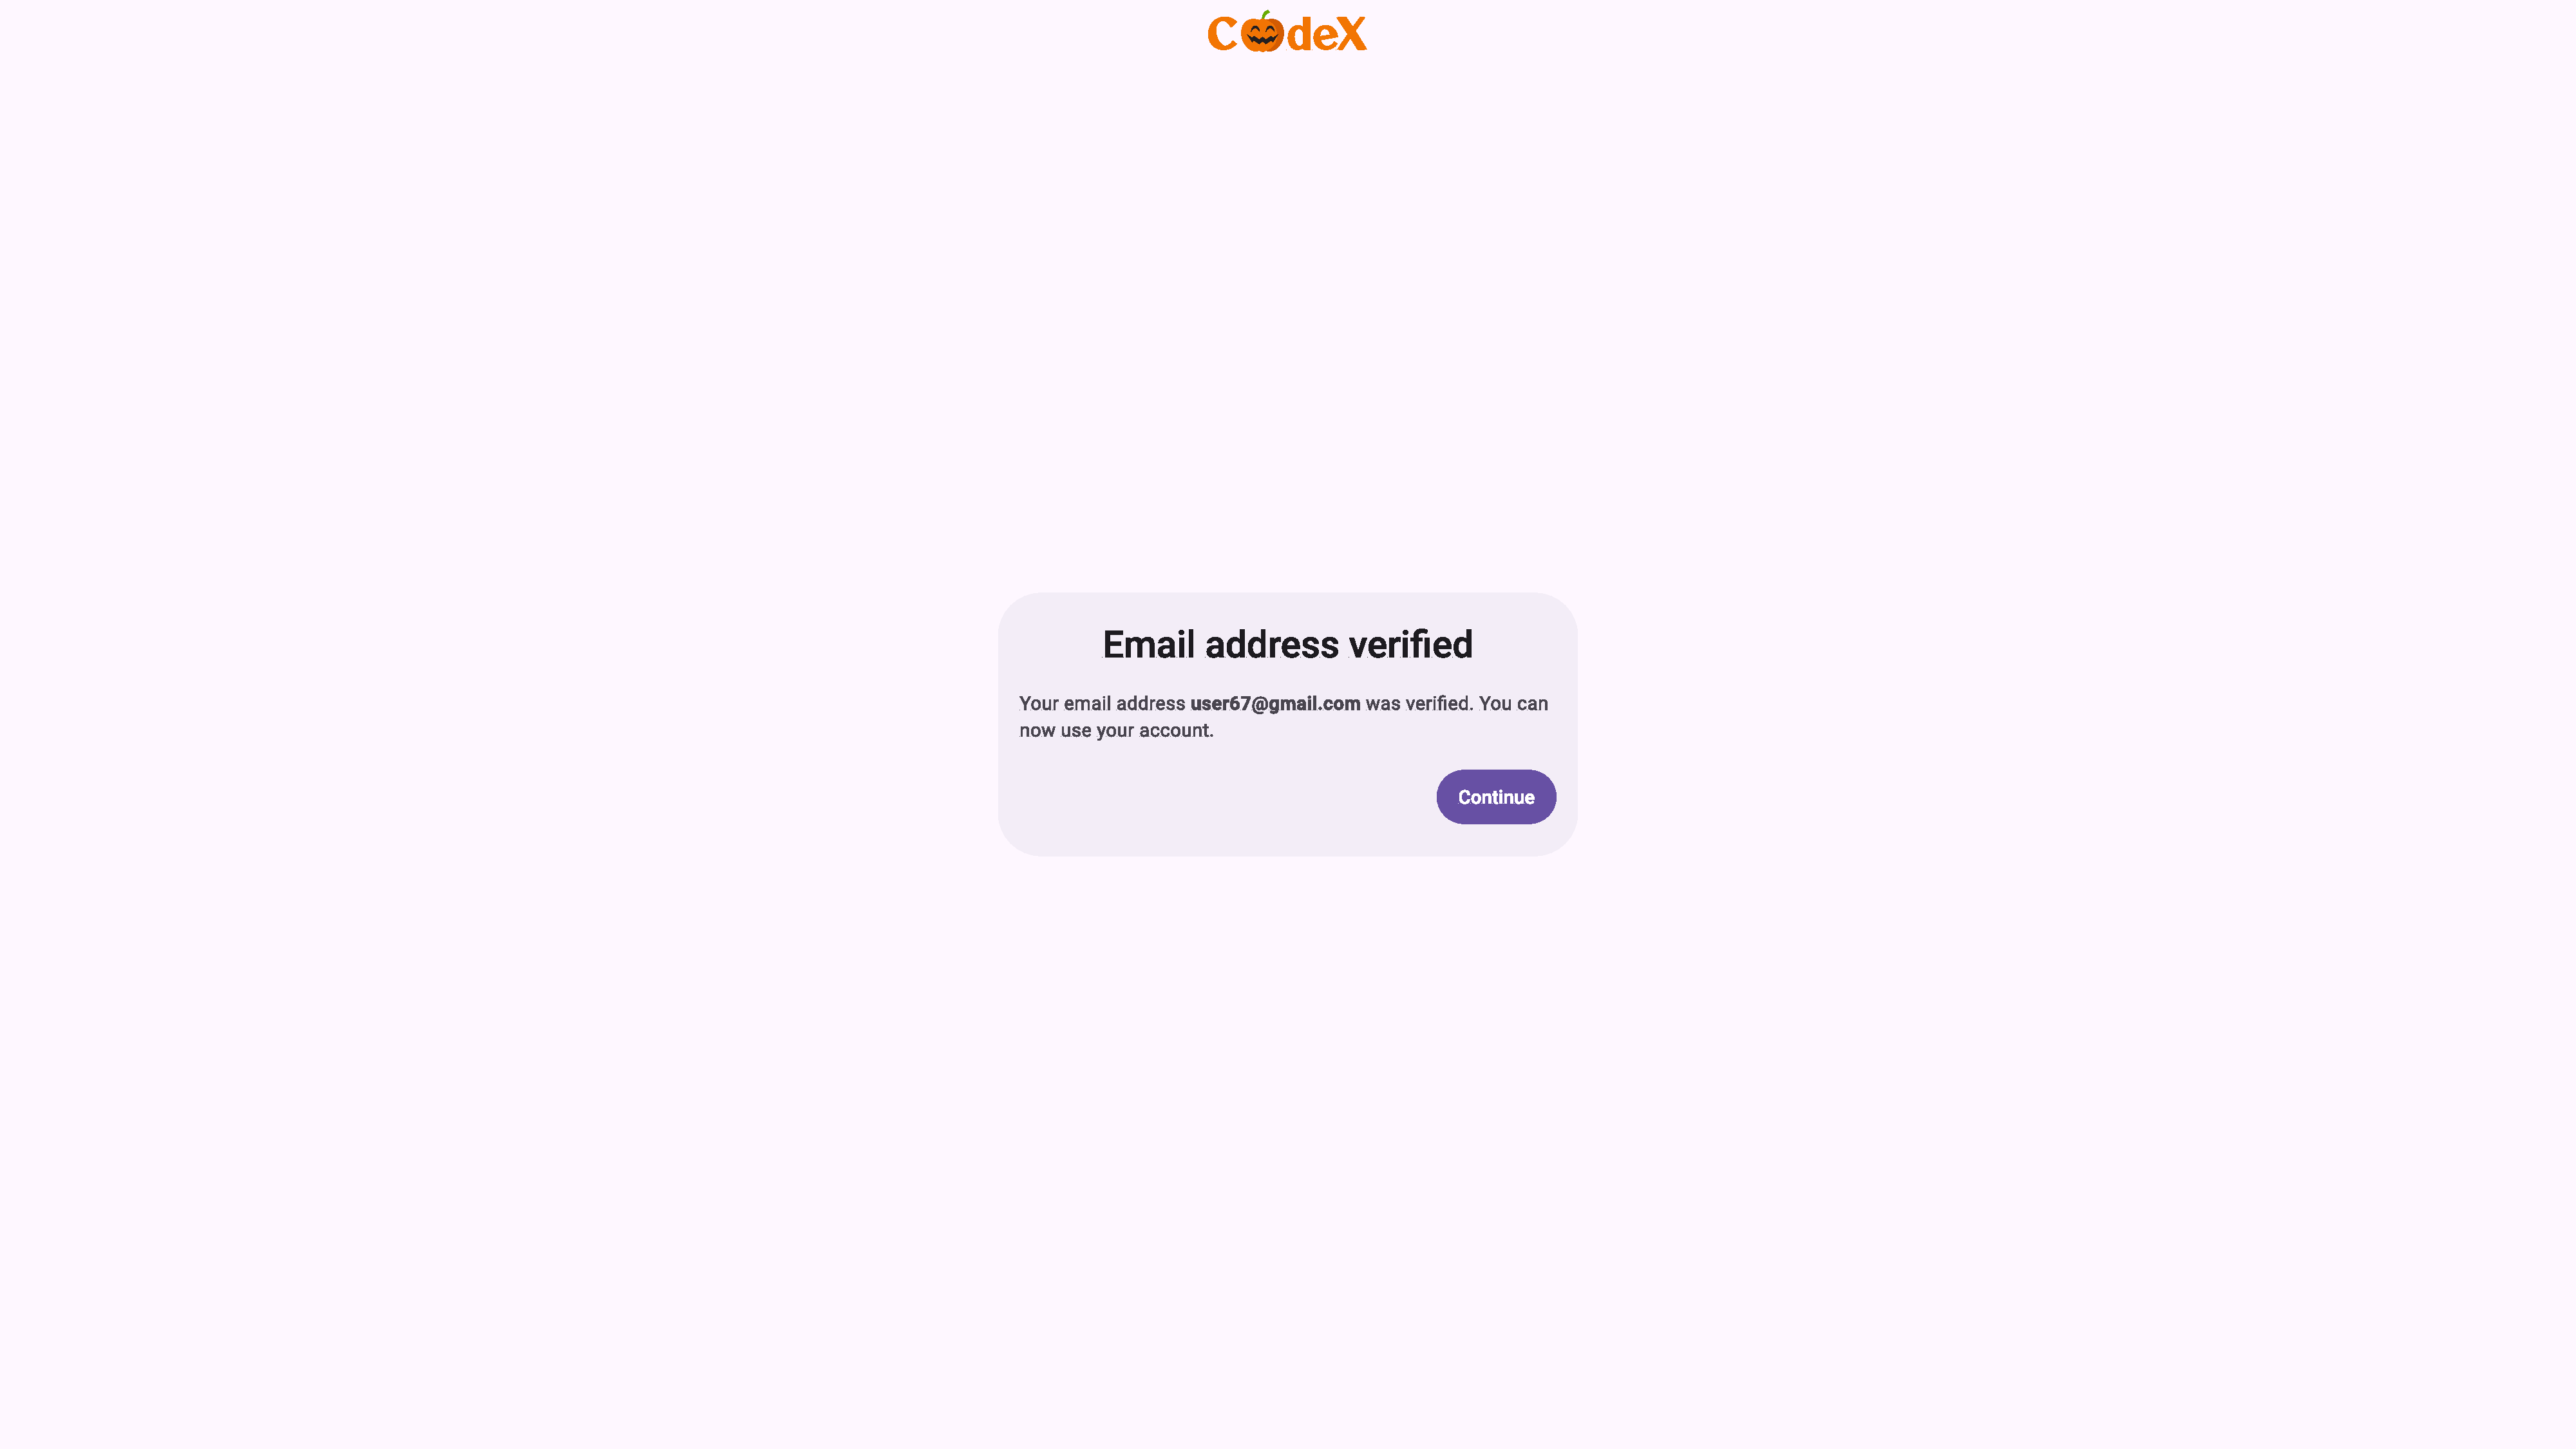
\includegraphics[width=\linewidth]{figures/ui/desktop/Email_Verification_Screen}
    \caption{\hyperref[abr:GUI]{GUI}: Verified screen}
    \label{fig:ui-d-verified}
\end{figure}
\begin{figure}
    \centering
    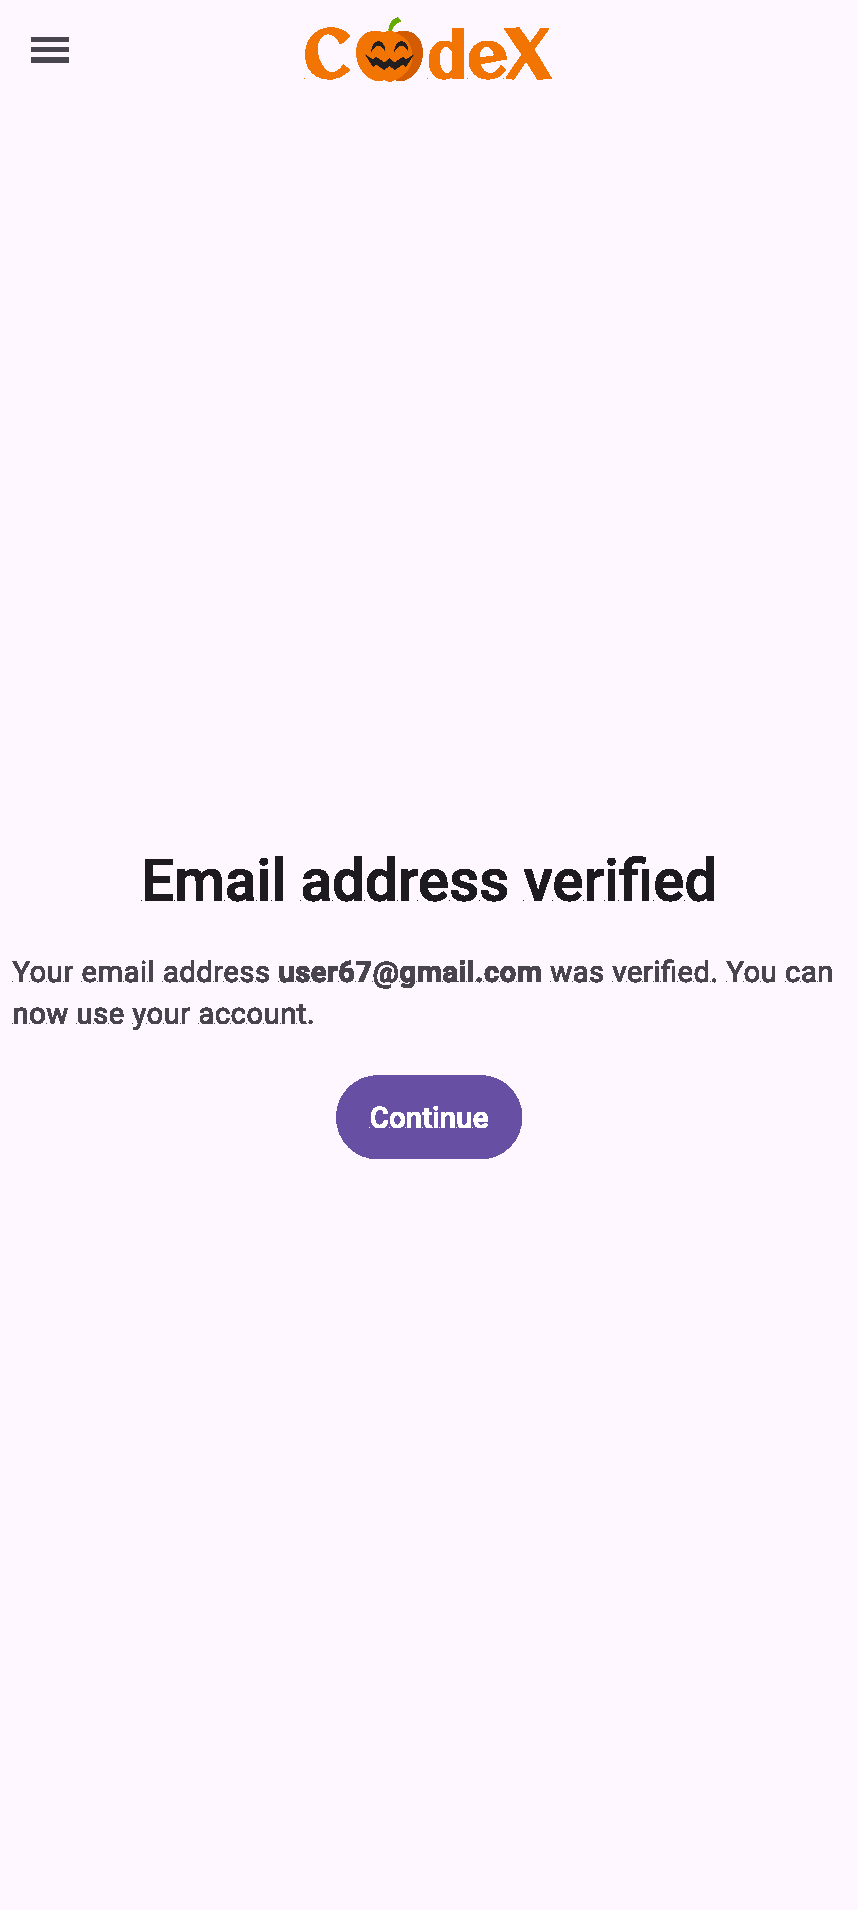
\includegraphics[width=5cm]{figures/ui/mobile/Email_Verification_Screen}
    \caption{\hyperref[abr:GUI]{GUI}: Verified screen (mobile)}
    \label{fig:ui-m-verified}
\end{figure}

\section{Modals}\label{sec:modals}
This section lists the modals, i.e. visual components that will be displayed as floating and over other components.
Namely, these are \textit{Dialog}s \footnote{https://m3.material.io/components/dialogs/overview} and \textit{Menu}s \footnote{https://m3.material.io/components/menus/overview}. \newline
These have the same layout and proportions on all screen sizes.

\subsection{Account dialog}
The account dialog is shown when users click the account settings button on the main screen. \newline
It displays information about the account, like username, email and current quota progress.
Actions like resetting the password or logging out are available. \newline
Depending on the role of the account, a dialog for  admin (\ref{fig:ui-d-account-dialog-admin}) or member (\ref{fig:ui-d-account-dialog-moderator}) is shown.
\begin{figure}
    \centering
    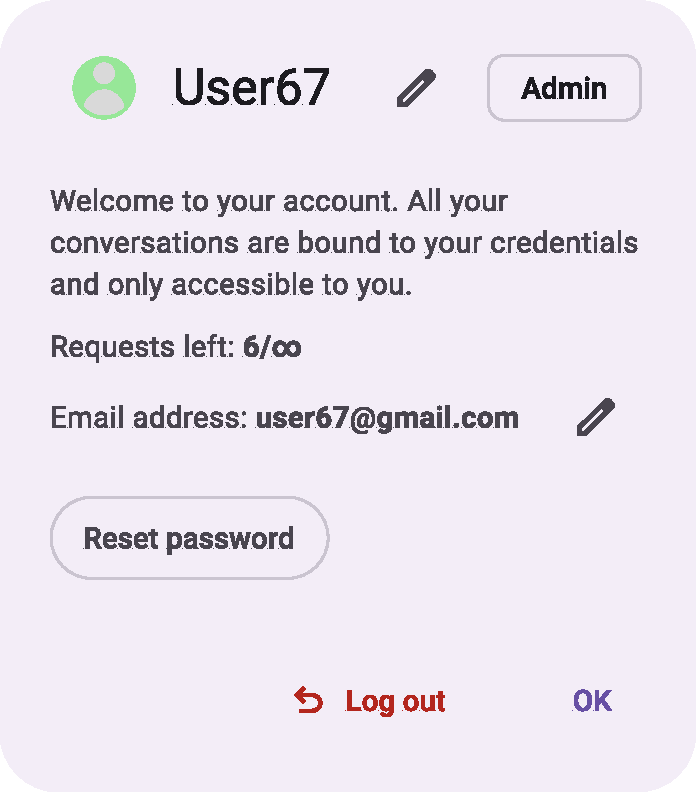
\includegraphics[width=5cm]{figures/ui/shared/Account_Dialog admin}
    \caption{\hyperref[abr:GUI]{GUI}: Account dialog for admin}
    \label{fig:ui-d-account-dialog-admin}
\end{figure}
\begin{figure}
    \centering
    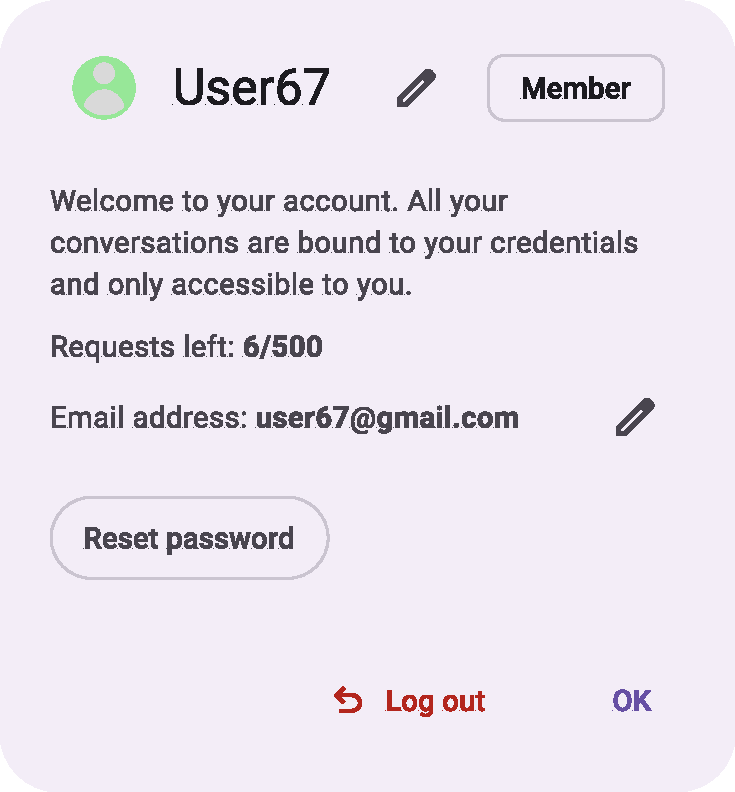
\includegraphics[width=5cm]{figures/ui/shared/Account_Dialog moderator}
    \caption{\hyperref[abr:GUI]{GUI}: Account dialog for user}
    \label{fig:ui-d-account-dialog-moderator}
\end{figure}

\subsection{Change username dialog}
The change username dialog (\ref{fig:ui-d-change-username-dialog}) allows a user to change the username of their account.
\begin{figure}
    \centering
    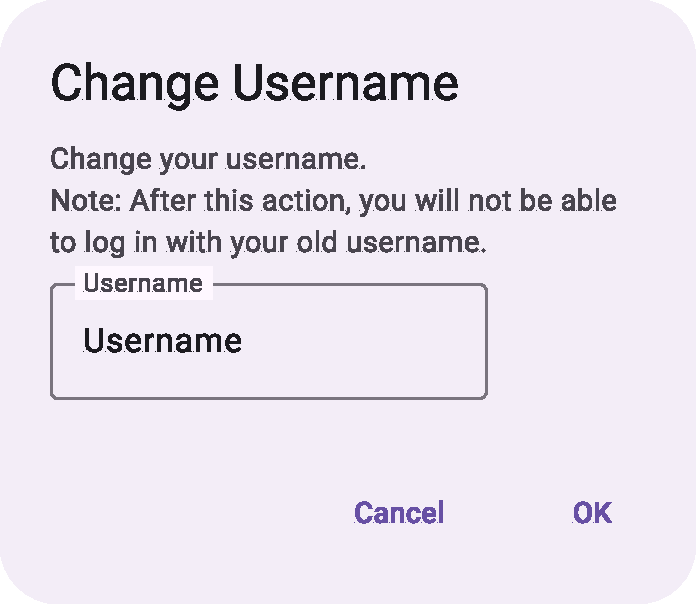
\includegraphics[width=5cm]{figures/ui/shared/Change_UsernameDialog}
    \caption{\hyperref[abr:GUI]{GUI}: Change username dialog}
    \label{fig:ui-d-change-username-dialog}
\end{figure}

\subsection{Change email dialog}
The change email dialog (\ref{fig:ui-d-change-email-dialog}) allows a user to change the email of their account. \newline
After the email was changed, the account is set to not verified again.
\begin{figure}
    \centering
    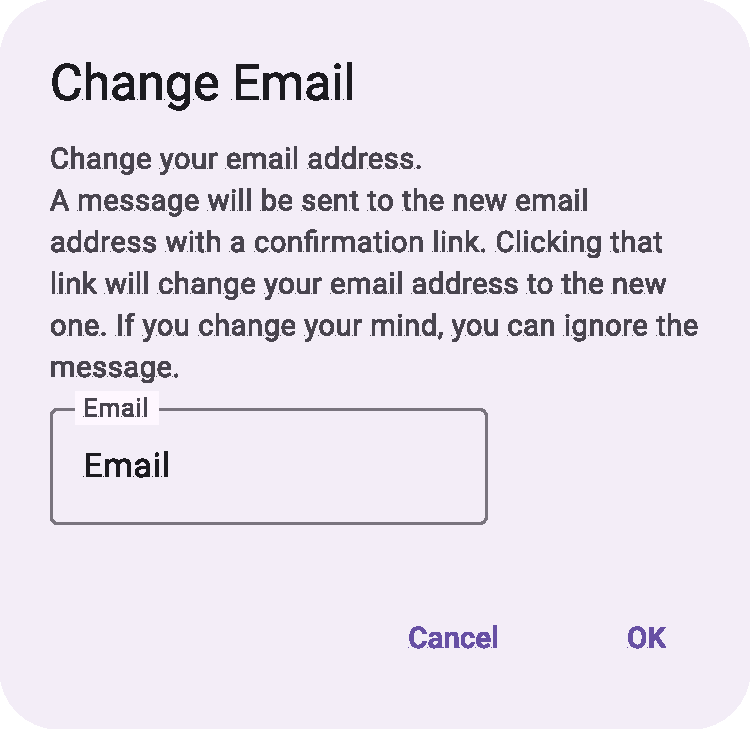
\includegraphics[width=5cm]{figures/ui/shared/Change_Email_Dialog}
    \caption{\hyperref[abr:GUI]{GUI}: Change email dialog}
    \label{fig:ui-d-change-email-dialog}
\end{figure}

\subsection{Conversation menu}
The conversation menu (\ref{fig:ui-d-conversation-menu}) is opened when the options button is clicked on a conversation item in the list of the main screen.
It allows a user to pin, rename or delete a conversation.
\begin{figure}
    \centering
    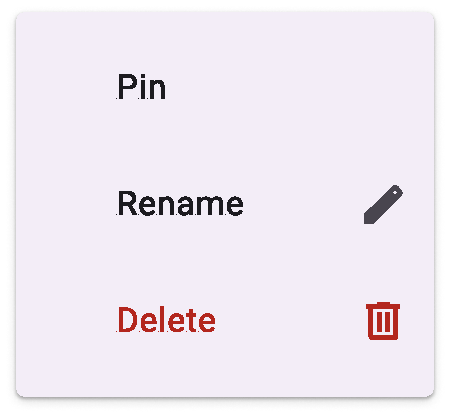
\includegraphics[width=3cm]{figures/ui/shared/Conversation_Menu}
    \caption{\hyperref[abr:GUI]{GUI}: Conversation menu}
    \label{fig:ui-d-conversation-menu}
\end{figure}
\section{Email}\label{sec:email}
In the following, we present the design for emails sent to the user. \newline
Due to the similar layout on mobile screens, the email-design is only presented for desktop devices.

\subsection{Password Reset Email}
Figure \ref{fig:ui_e_reset_password} shows the email sent to the user when the password is reset.
It contains a link to the web-interface.
\begin{figure}
    \centering
    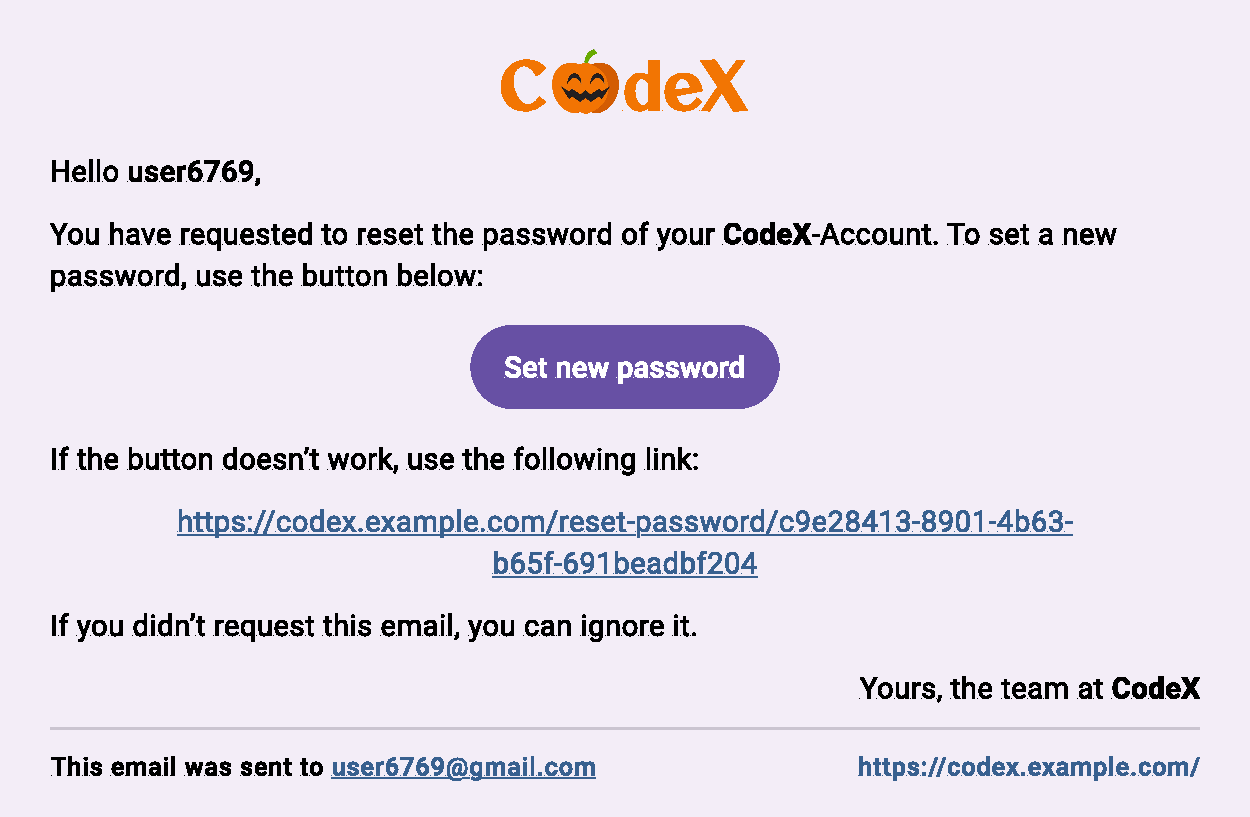
\includegraphics[width=\linewidth]{figures/ui/email/Password_Reset_Email}
    \caption{\hyperref[abr:GUI]{GUI}: Email for resetting password}
    \label{fig:ui_e_reset_password}
\end{figure}

\subsection{Email Verication Email}
Figure \ref{fig:ui_e_email_verify} shows the email sent to the user when their email needs to be verified.
It contains a link to the web-interface.
\begin{figure}
    \centering
    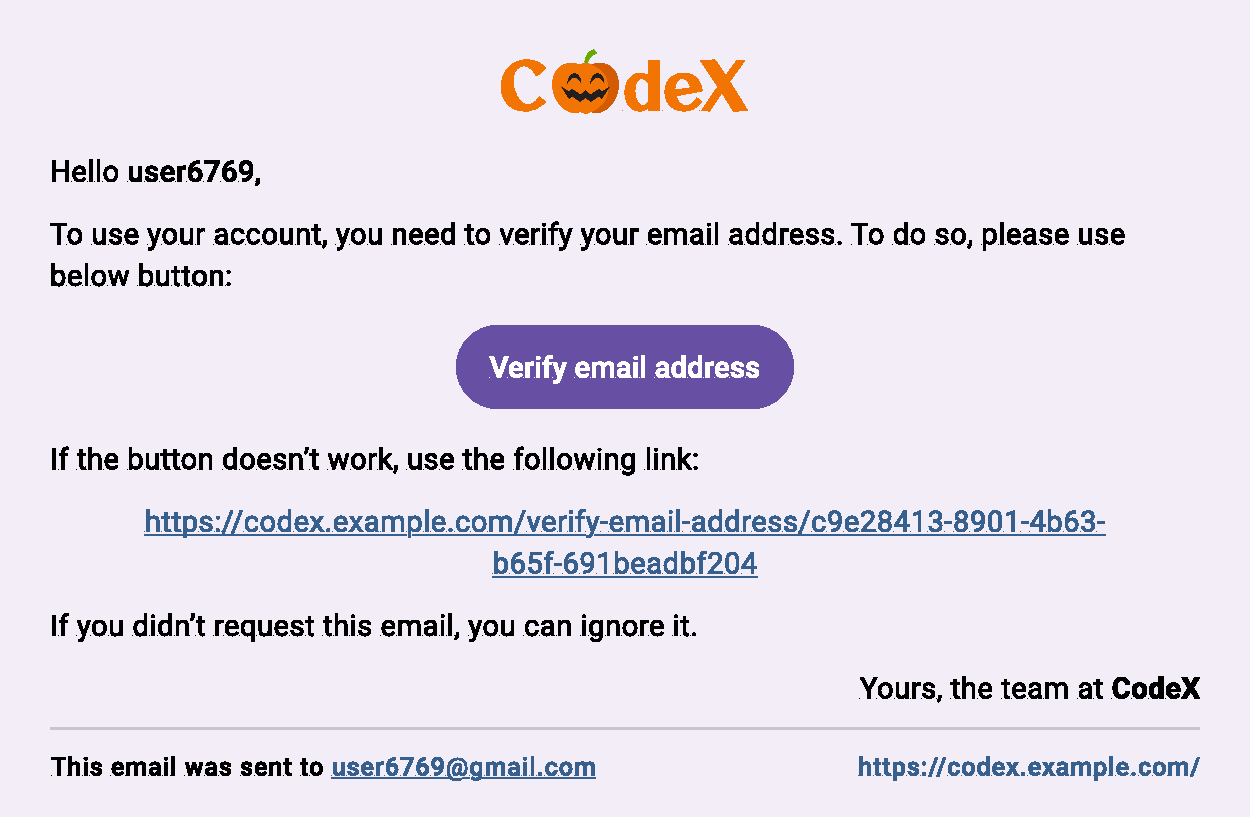
\includegraphics[width=\linewidth]{figures/ui/email/Email_Verify_Email}
    \caption{\hyperref[abr:GUI]{GUI}: Email for verifying email address}
    \label{fig:ui_e_email_verify}
\end{figure}